\section{Preventivo}
In questa sezione del documento viene riportata la distribuzione delle risorse del gruppo nelle varie fasi di lavoro.\\
Inoltre sono illustrate la pianificazione e distribuzione oraria dei ruoli per ogni membro del gruppo, i quali devono:
\begin{itemize}
	\item Ricoprire tutti i ruoli durante tutta la durata del progetto;
	\item Avere circa le stesse ore produttive alla fine di ogni fase del progetto.
\end{itemize}
Inoltre il verificatore di un determinato task non potrà essere colui che lo ha svolto.\\
Il riferimento alle sigle identificative dei ruoli si può trovare al paragrafo 3.1.5.5 del documento \textbf{Norme di progetto v0.0.7}.
\newpage
\subsection{Analisi}
%
% ----------------------------------------------------------------------------------------------------------------
\subsubsection{Periodo 1}
% ----------------------------------------------------------------------------------------------------------------
%
\subsubsubsection{Preventivo orario}
La seguente tabella rappresenta la distribuzione oraria per ogni componente per il primo periodo della fase di Analisi:

	\setlength\extrarowheight{5pt}
	\rowcolors{2}{gray!10}{gray!40}
	\begin{tabularx}{\textwidth}{|ccccccc|c|}
		\hline
		\rowcolor{white}
		\textbf{Nome} & \textbf{Re} & \textbf{Am} & \textbf{An} & \textbf{Ve} & \textbf{Pr}& \textbf{Pt} & \textbf{Ore totali} \\
		\hline
		Nicola Sinicato &3&3&4&0&0&0&10 \\
		Gabriele Da Re &0&6&4&0&0&0&10 \\
		Luca Brugnera &0&6&4&0&0&0&10 \\
		Matteo Stocco &1&5&4&0&0&0&10 \\
		Ana Lazic &1&3&6&0&0&0&10 \\
		Zhen Wei Zheng &1&3&6&0&0&0&10 \\
		\hline
		Ore totali ruolo &6&26&28&0&0&0&60 \\
		\hline
		\rowcolor{white}
		\caption{ Distribuzione oraria durante il primo periodo di analisi per ruolo e persona}
	\end{tabularx}
	\vspace{10pt}
	

\begin{figure}[H]
    \centering
    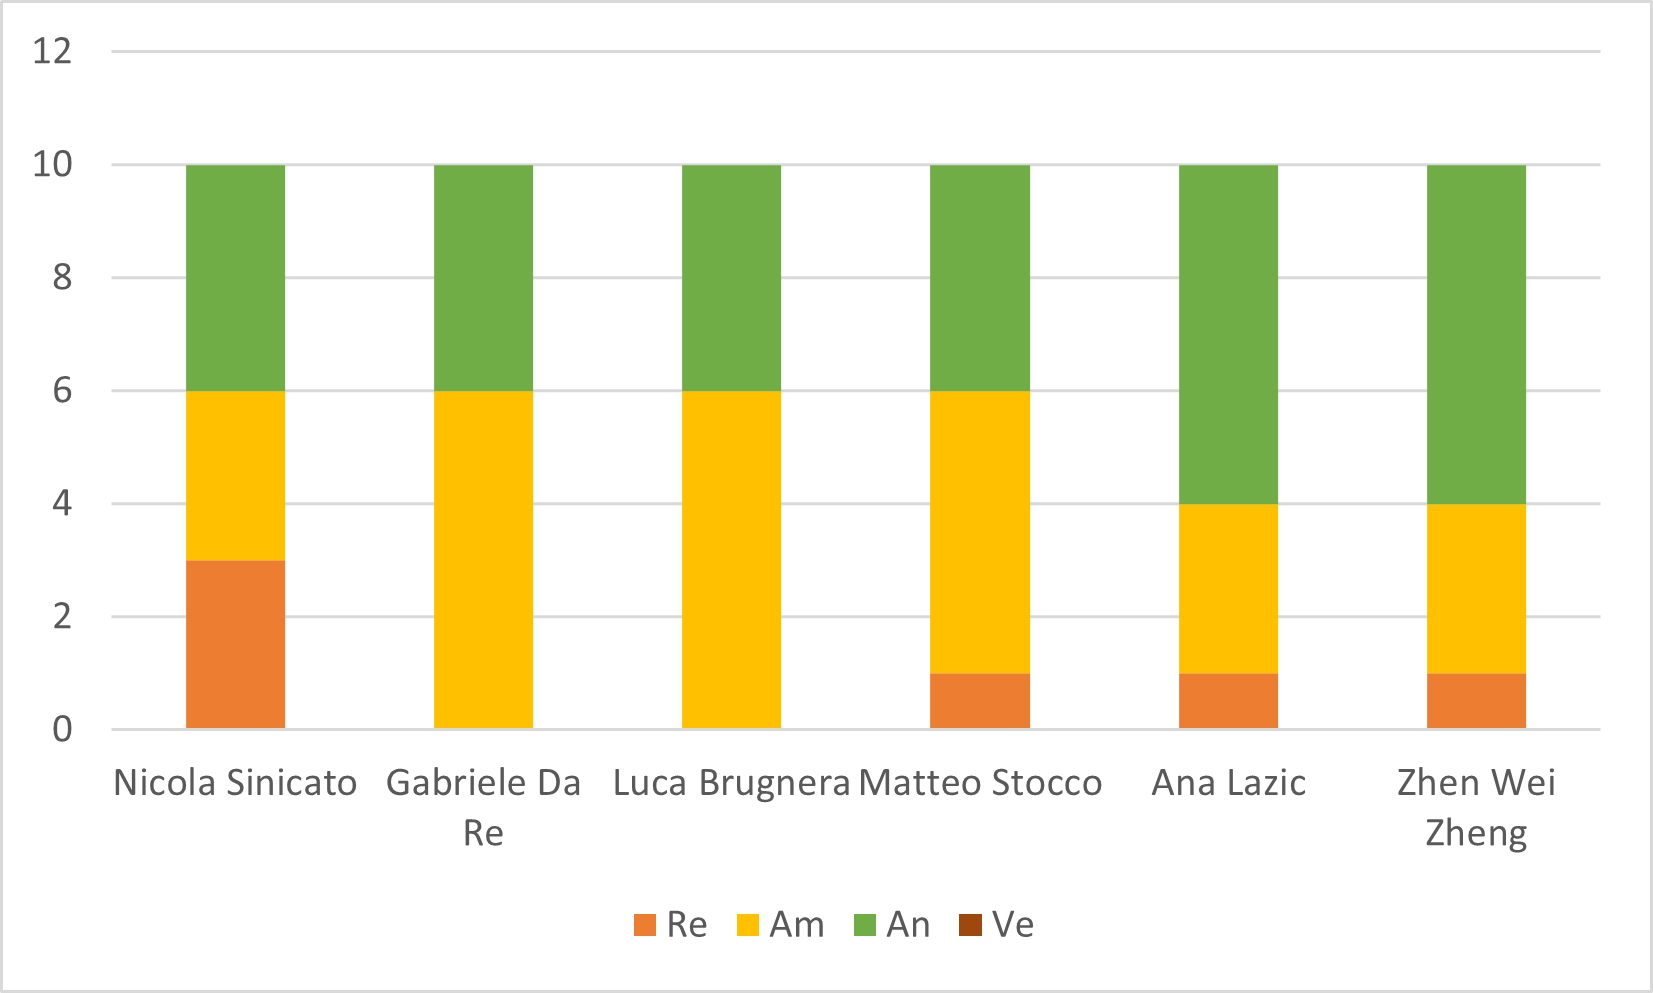
\includegraphics[scale=0.6]{img/grafi preventivo/istogrammi/analisi/periodo1.png}
    \caption{Istogramma della ripartizione delle ore del primo periodo della fase di analisi}
\end{figure}
\begin{figure}[H]
    \centering
    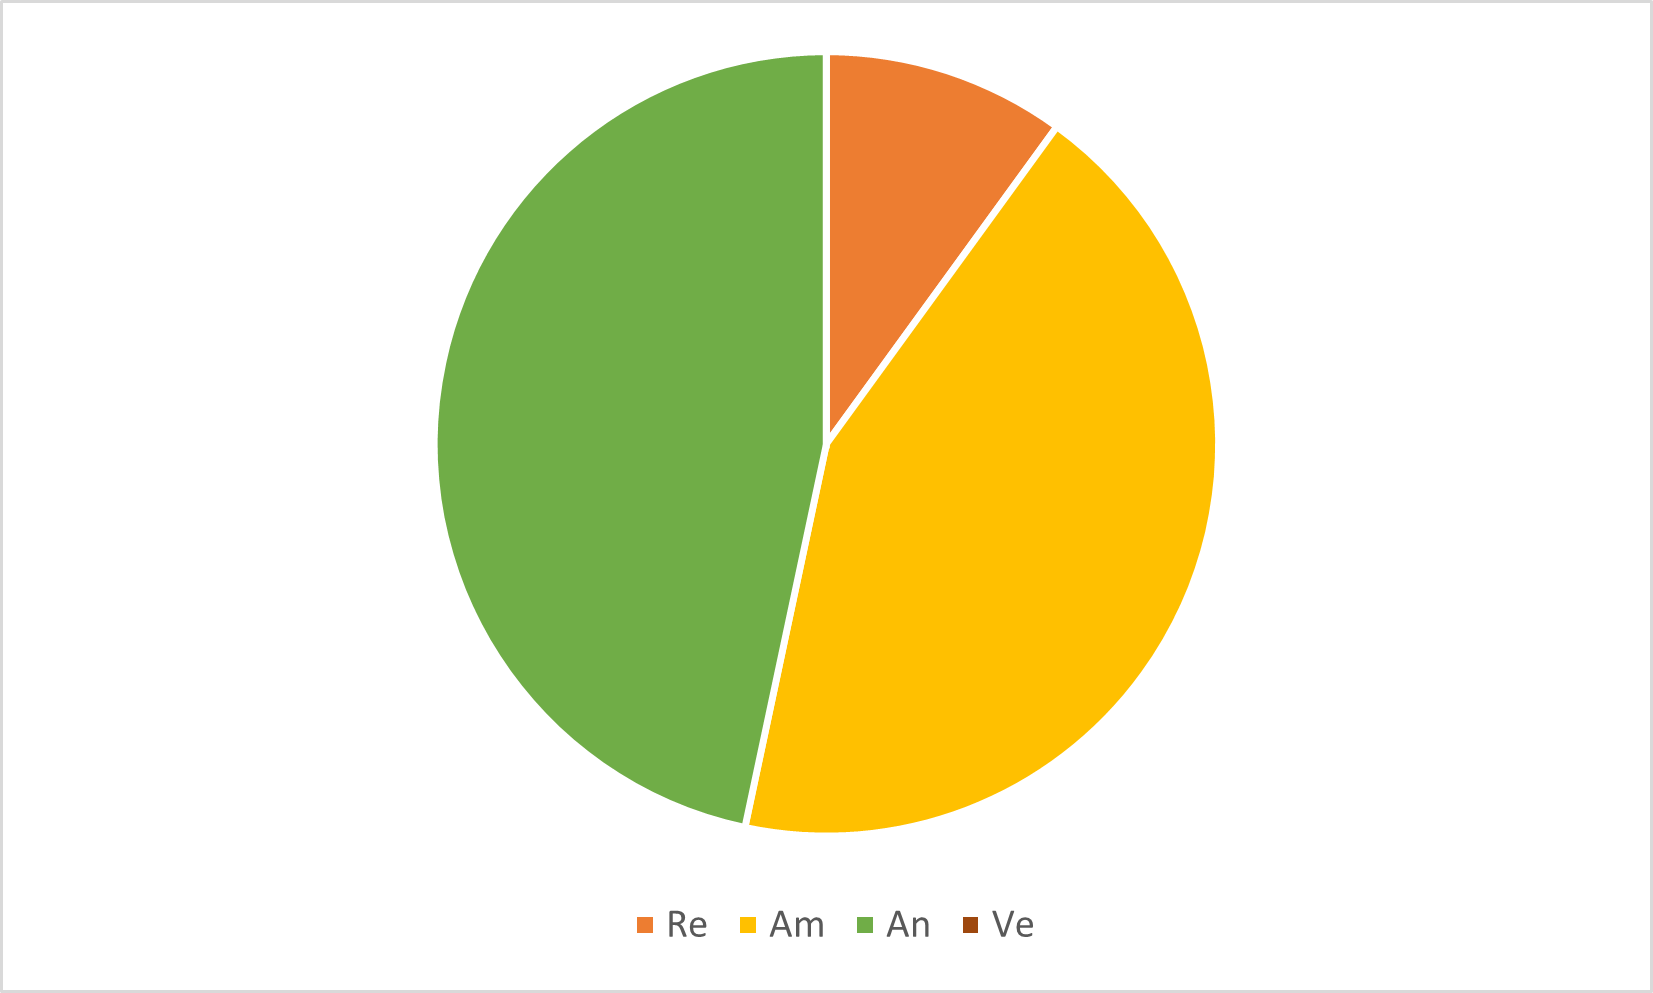
\includegraphics[scale=0.6]{img/grafi preventivo/torta/analisi/periodo1.png}
    \caption{Grafico a torta della ripartizione delle ore per ruolo nel primo periodo della fase di analisi}
\end{figure}

\subsubsubsection{Preventivo dei costi}
La seguente tabella rappresenta le ore dedicate ad ogni ruolo e il corrispettivo costo in euro per il primo periodo della fase di analisi:

	\setlength\extrarowheight{5pt}
	\rowcolors{2}{gray!10}{gray!40}
	\begin{tabularx}{\textwidth}{|ccc|c|}
		\hline
		\rowcolor{white}
		\textbf{Ruolo} & \textbf{Costo orario (€)} & \textbf{Ore totali} & \textbf{Costo totale (€)} \\
		\hline
		Responsabile &30&6&180 \\
		Amministratore &20&26&520 \\
		Analista &25&28&700 \\
		Verificatore &15&0&0 \\
		Programmatore &15&0&0 \\
		Progettista &25&0&0 \\
		\hline
		Totale &-&-&1400 \\
		\hline
		\rowcolor{white}
		\caption{Prospetto del costo orario durante il primo periodo di analisi per ruolo}
	\end{tabularx}
    \vspace{10pt}
	
% ----------------------------------------------------------------------------------------------------------------
\newpage
\subsubsection{Periodo 2}
% ----------------------------------------------------------------------------------------------------------------
%
\subsubsubsection{Preventivo orario}
La seguente tabella rappresenta la distribuzione oraria per ogni componente per il secondo periodo della fase di analisi:

	\setlength\extrarowheight{5pt}
	\rowcolors{2}{gray!10}{gray!40}
	\begin{tabularx}{\textwidth}{|ccccccc|c|}
		\hline
		\rowcolor{white}
		\textbf{Nome} & \textbf{Re} & \textbf{Am} & \textbf{An} & \textbf{Ve} & \textbf{Pr}& \textbf{Pt} & \textbf{Ore totali} \\
		\hline
		Nicola Sinicato &2&1&8&4&0&0&15 \\
		Gabriele Da Re &1&4&7&3&0&0&15 \\
		Luca Brugnera &1&5&6&3&0&0&15 \\
		Matteo Stocco &2&2&7&4&0&0&15 \\
		Ana Lazic &0&2&7&6&0&0&15 \\
		Zhen Wei Zheng &0&2&6&7&0&0&15 \\
		\hline
		Ore totali ruolo &6&16&41&27&0&0&90 \\
		\hline
		\rowcolor{white}
		\caption{Distribuzione oraria durante il secondo periodo di analisi per ruolo e persona}
	\end{tabularx}
	\vspace{10pt}
	
\begin{figure}[H]
    \centering
    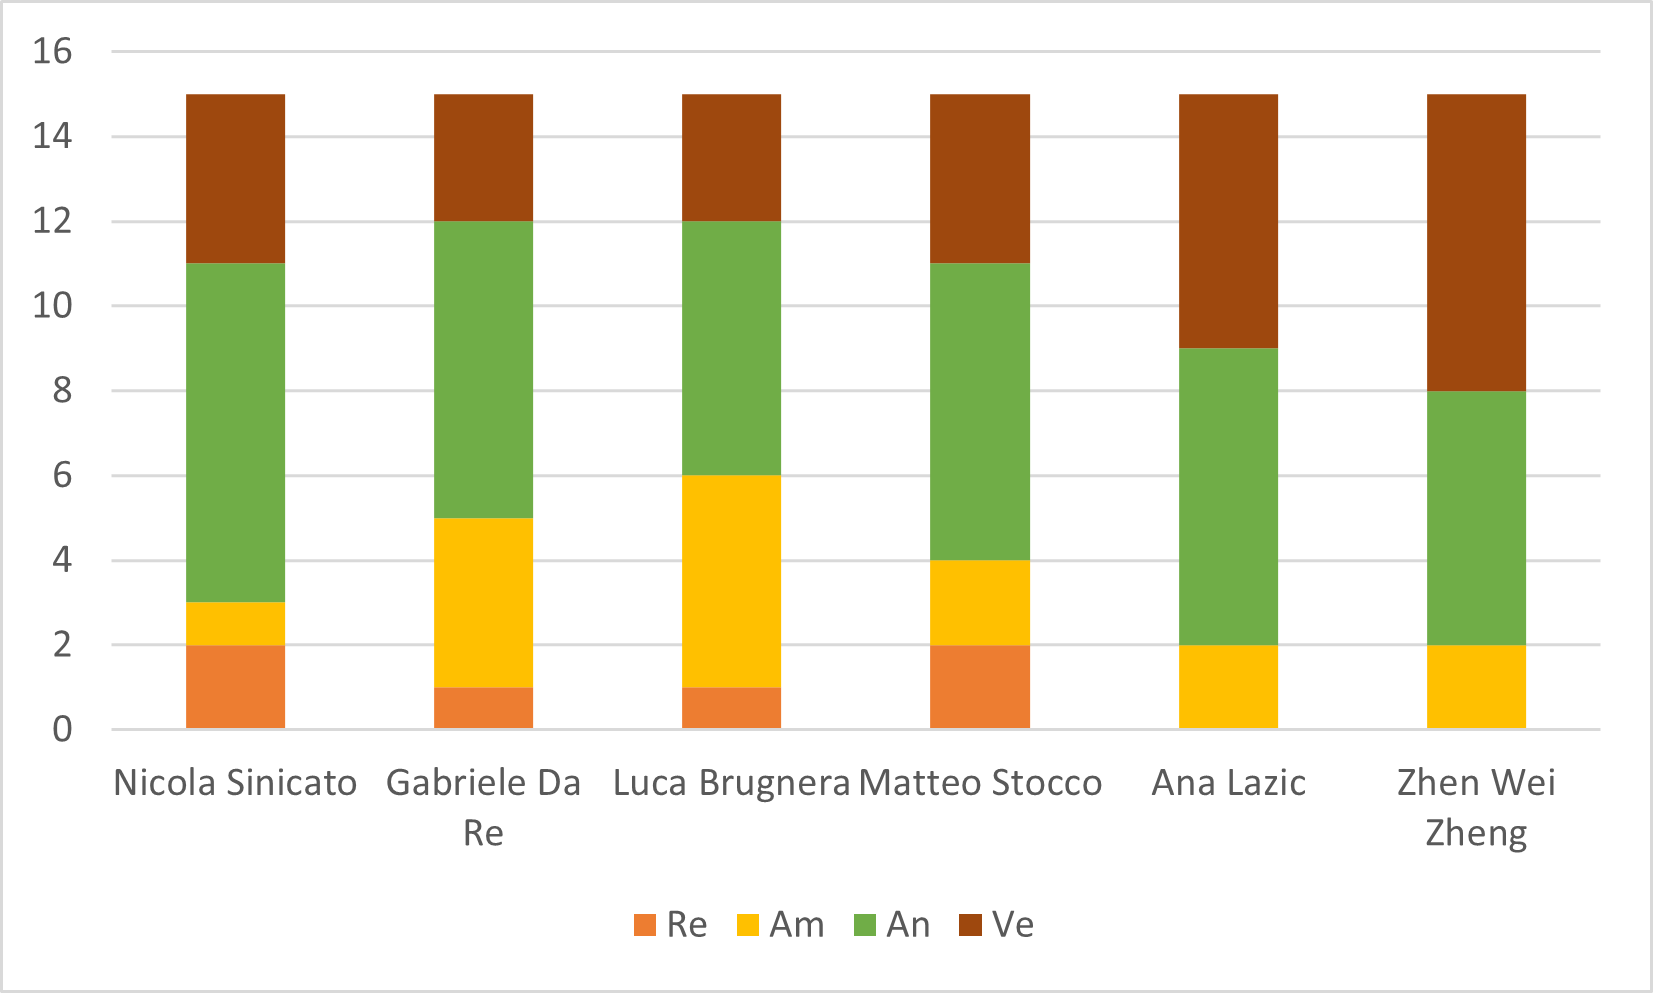
\includegraphics[scale=0.6]{img/grafi preventivo/istogrammi/analisi/periodo2.png}
    \caption{Istogramma della ripartizione delle ore del secondo periodo della fase di analisi}
\end{figure}
\begin{figure}[H]
    \centering
    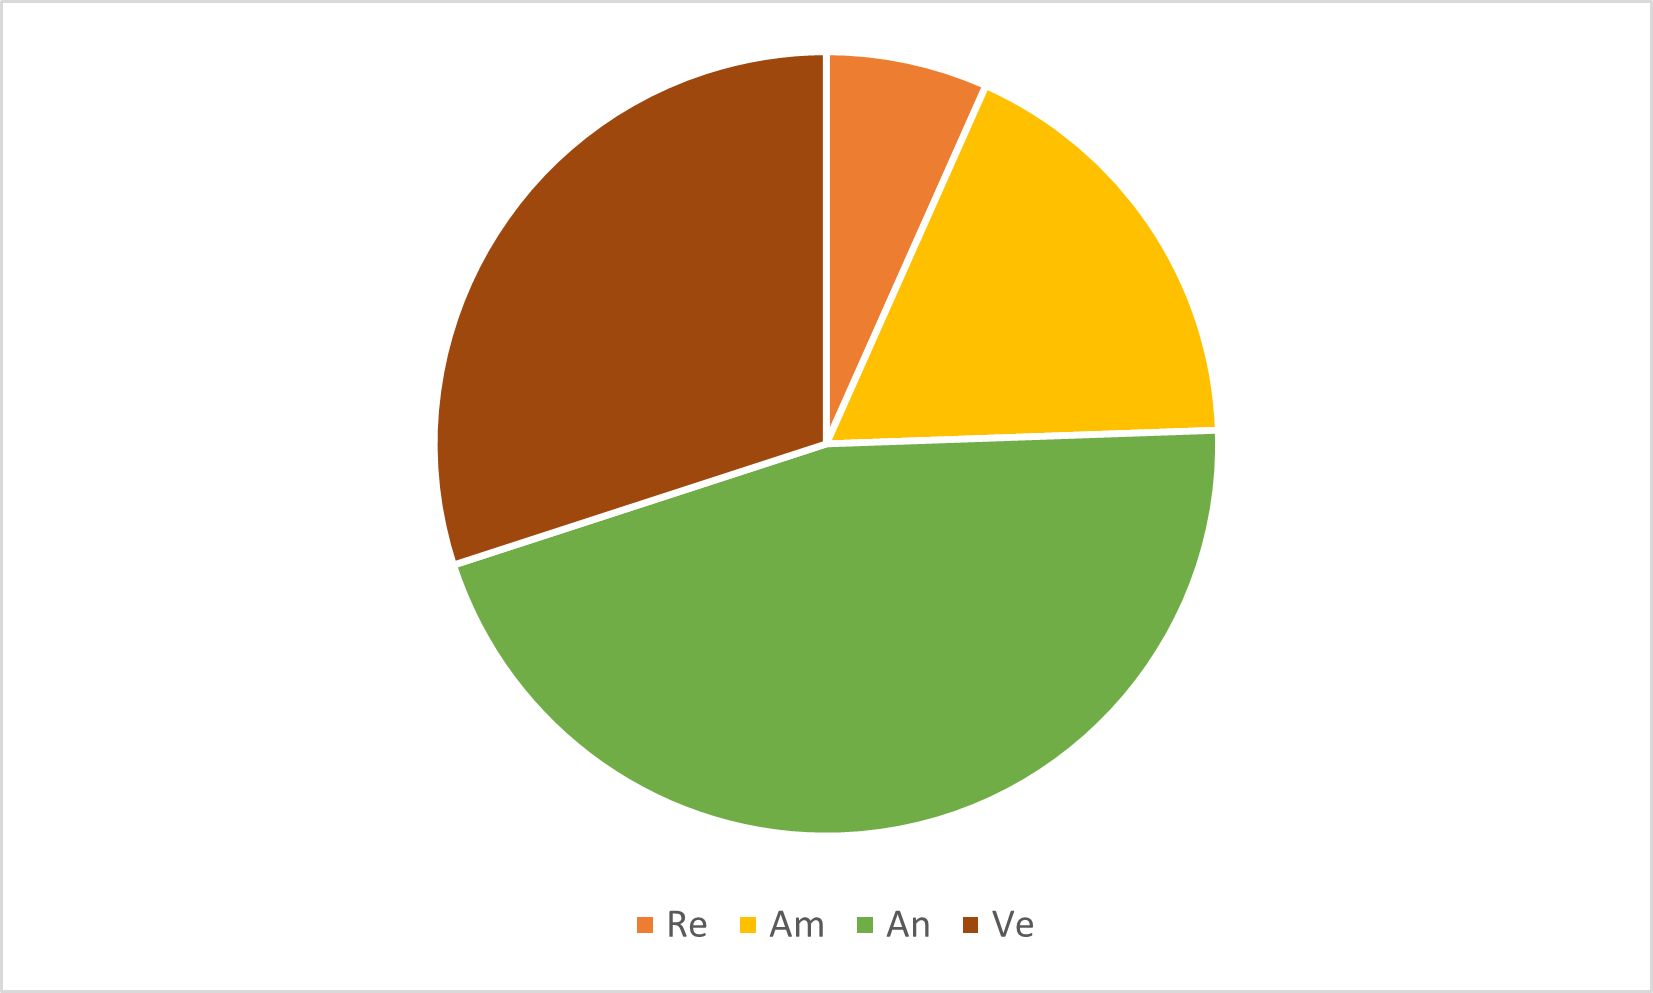
\includegraphics[scale=0.6]{img/grafi preventivo/torta/analisi/periodo2.png}
    \caption{Grafico a torta della ripartizione delle ore per ruolo nel secondo periodo della fase di analisi}
\end{figure}
\subsubsubsection{Preventivo dei costi}
La seguente tabella rappresenta le ore dedicate ad ogni ruolo e il corrispettivo costo in euro per il secondo periodo della fase di analisi:

	\setlength\extrarowheight{5pt}
	\rowcolors{2}{gray!10}{gray!40}
	\begin{tabularx}{\textwidth}{|ccc|c|}
		\hline
		\rowcolor{white}
		\textbf{Ruolo} & \textbf{Costo orario (€)} & \textbf{Ore totali} & \textbf{Costo totale (€)} \\
		\hline
		Responsabile &30&6&180 \\
		Amministratore &20&16&320 \\
		Analista &25&41&1025 \\
		Verificatore &15&27&405 \\
		Programmatore &15&0&0 \\
		Progettista &25&0&0 \\
		\hline
		Totale &-&-&1930 \\
		\hline
		\rowcolor{white}
		\caption{Prospetto del costo orario durante il secondo periodo di analisi per ruolo}
	\end{tabularx}
    \vspace{10pt}
	
%
% ----------------------------------------------------------------------------------------------------------------
\newpage
\subsubsection{Periodo 3}
% ----------------------------------------------------------------------------------------------------------------
%
\subsubsubsection{Preventivo orario}
La seguente tabella rappresenta la distribuzione oraria per ogni componente per il terzo periodo della fase di analisi:

	\setlength\extrarowheight{5pt}
	\rowcolors{2}{gray!10}{gray!40}
	\begin{tabularx}{\textwidth}{|ccccccc|c|}
		\hline
		\rowcolor{white}
		\textbf{Nome} & \textbf{Re} & \textbf{Am} & \textbf{An} & \textbf{Ve} & \textbf{Pr}& \textbf{Pt} & \textbf{Ore totali} \\
		\hline
		Nicola Sinicato &0&1&2&2&0&0&5 \\
		Gabriele Da Re &1&2&1&1&0&0&5 \\
		Luca Brugnera &0&2&1&2&0&0&5 \\
		Matteo Stocco &1&0&2&2&0&0&5 \\
		Ana Lazic &1&0&3&1&0&0&5 \\
		Zhen Wei Zheng &0&0&2&3&0&0&5 \\
		\hline
		Ore totali ruolo &3&5&11&11&0&0&30 \\
		\hline
		\rowcolor{white}
		\caption{Distribuzione oraria durante il terzo periodo di analisi per ruolo e persona}
	\end{tabularx}
	\vspace{10pt}
	
\begin{figure}[H]
    \centering
    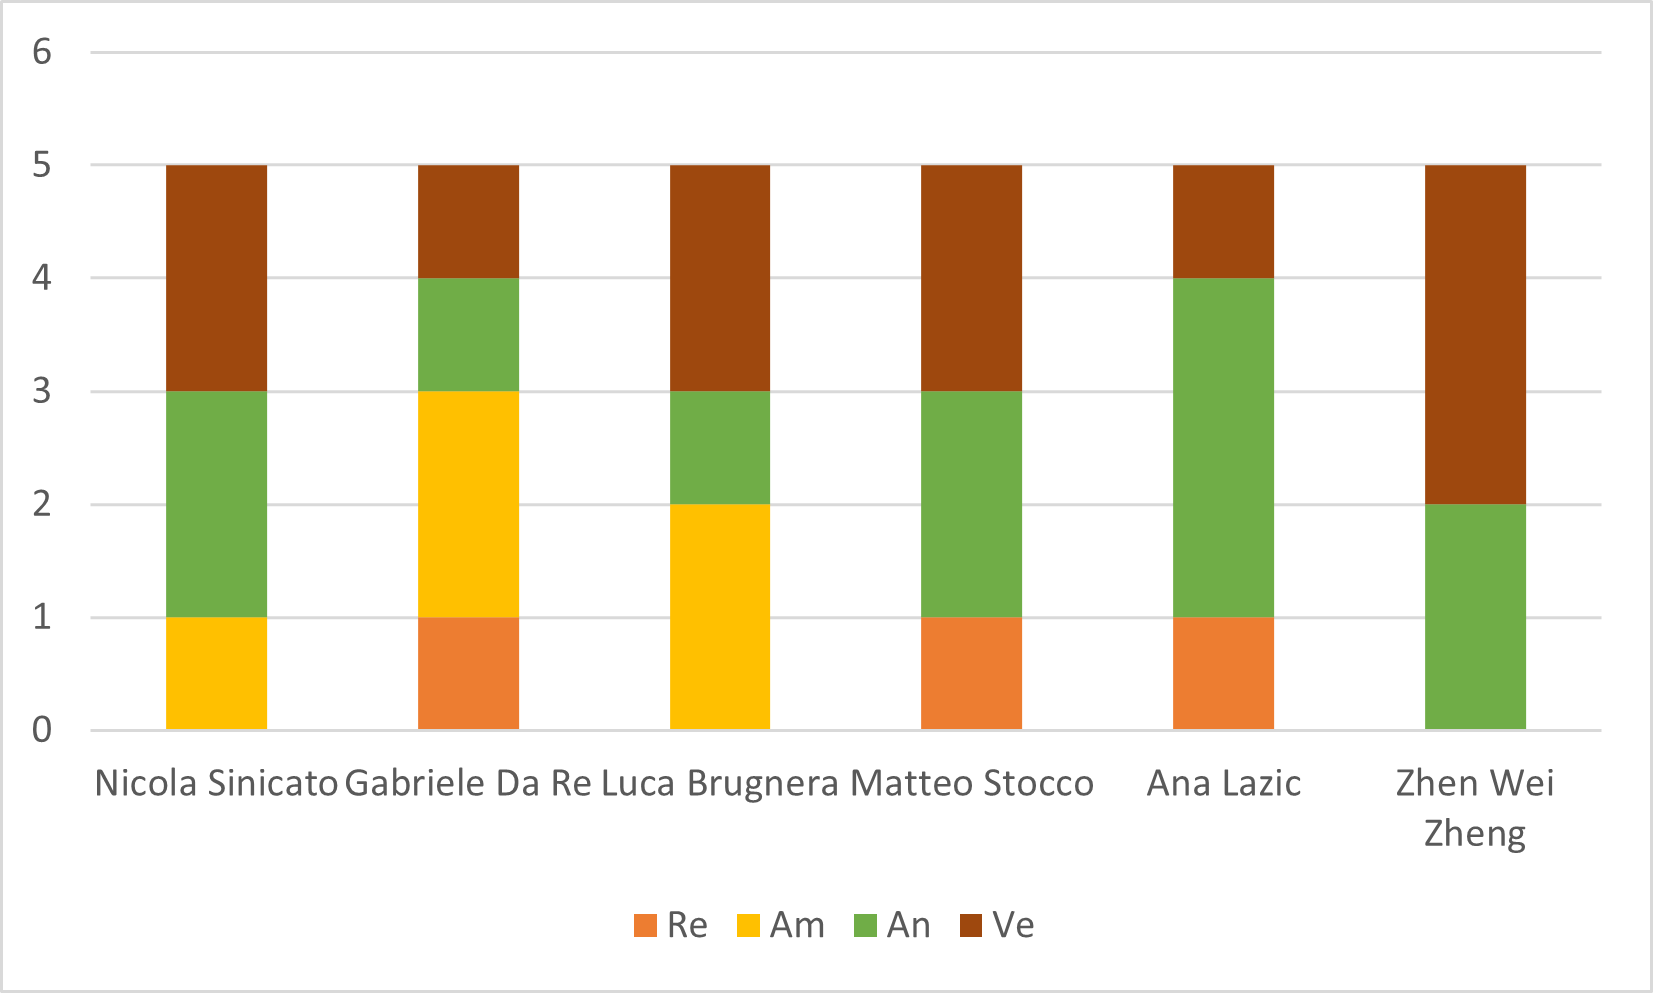
\includegraphics[scale=0.6]{img/grafi preventivo/istogrammi/analisi/periodo3.png}
    \caption{Istogramma della ripartizione delle ore del terzo periodo della fase di analisi}
\end{figure}
\begin{figure}[H]
    \centering
    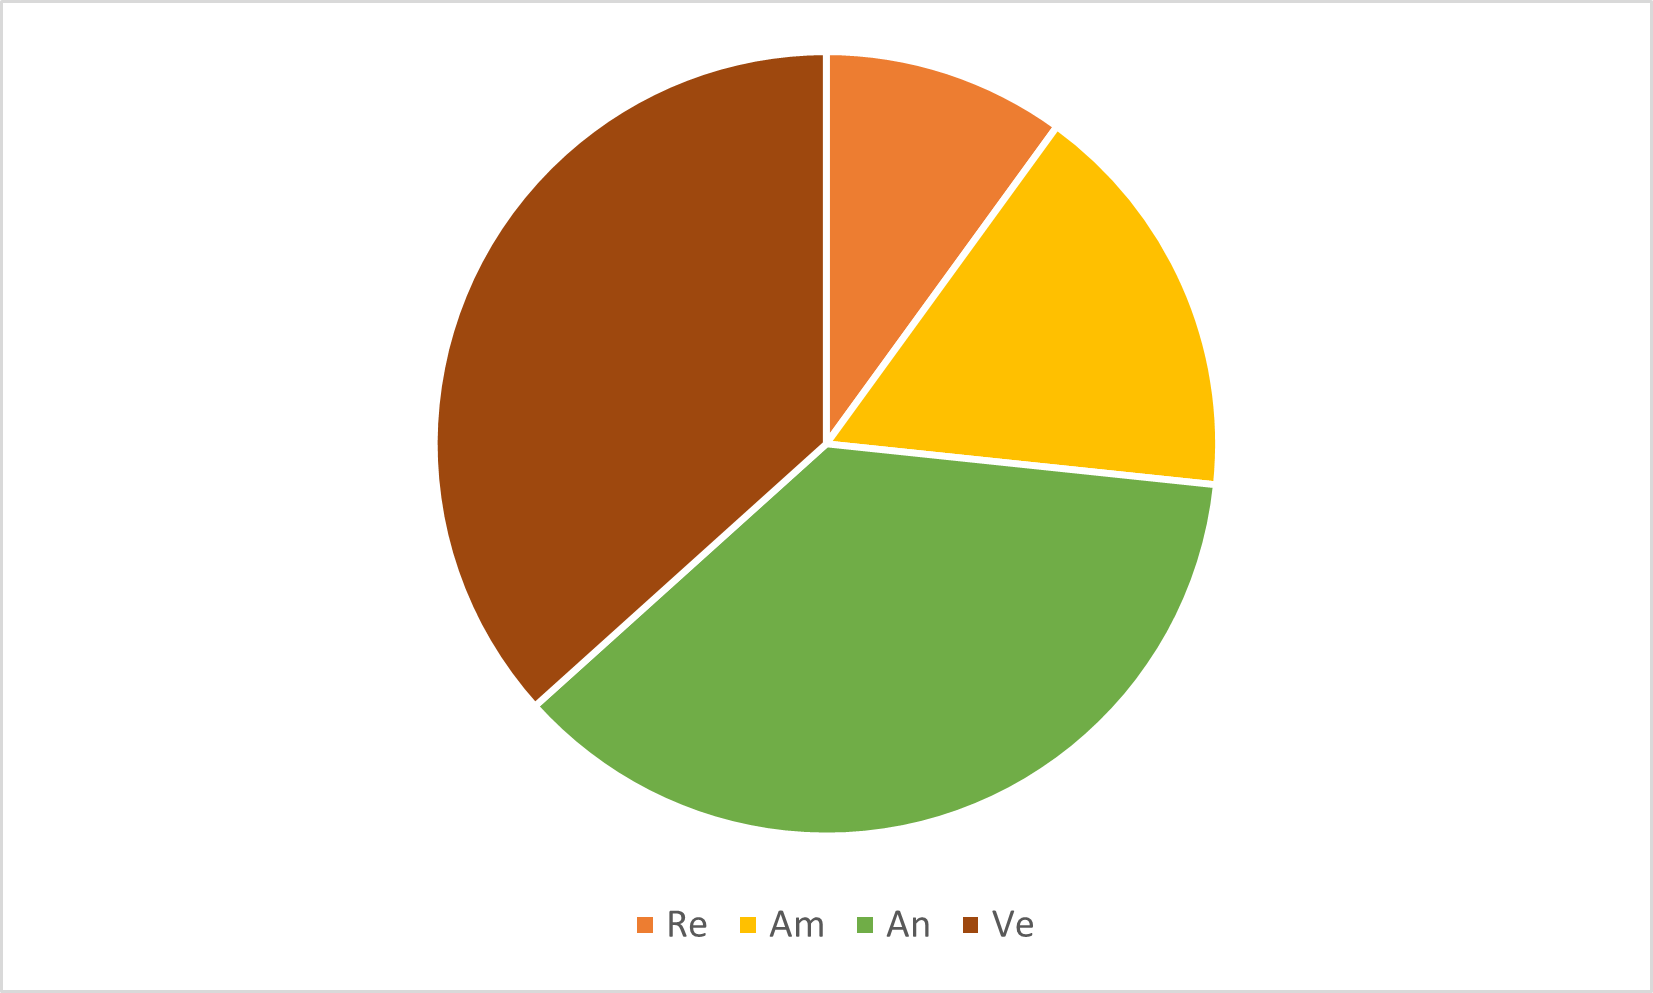
\includegraphics[scale=0.6]{img/grafi preventivo/torta/analisi/periodo3.png}
    \caption{Grafico a torta della ripartizione delle ore per ruolo nel terzo periodo della fase di analisi}
\end{figure}
\subsubsubsection{Preventivo dei costi}
La seguente tabella rappresenta le ore dedicate ad ogni ruolo e il corrispettivo costo in euro per il terzo periodo della fase di analisi:

	\setlength\extrarowheight{5pt}
	\rowcolors{2}{gray!10}{gray!40}
	\begin{tabularx}{\textwidth}{|ccc|c|}
		\hline
		\rowcolor{white}
		\textbf{Ruolo} & \textbf{Costo orario (€)} & \textbf{Ore totali} & \textbf{Costo totale (€)} \\
		\hline
		Responsabile &30&3&90 \\
		Amministratore &20&5&100 \\
		Analista &25&11&275 \\
		Verificatore &15&11&165 \\
		Programmatore &15&0&0 \\
		Progettista &25&0&0 \\
		\hline
		Totale &-&-&630 \\
		\hline
		\rowcolor{white}
		\caption{Prospetto del costo orario durante il terzo periodo di analisi per ruolo}
	\end{tabularx}
    \vspace{10pt}
	
%
% ----------------------------------------------------------------------------------------------------------------
\newpage
\subsubsection{Riepilogo della fase di analisi}
% ----------------------------------------------------------------------------------------------------------------
%
\subsubsubsection{Preventivo orario}
La seguente tabella rappresenta la distribuzione oraria per ogni componente per la fase di analisi:

	\setlength\extrarowheight{5pt}
	\rowcolors{2}{gray!10}{gray!40}
	\begin{tabularx}{\textwidth}{|ccccccc|c|}
		\hline
		\rowcolor{white}
		\textbf{Nome} & \textbf{Re} & \textbf{Am} & \textbf{An} & \textbf{Ve} & \textbf{Pr}& \textbf{Pt} & \textbf{Ore totali} \\
		\hline
		Nicola Sinicato &5&5&14&6&0&0&30 \\
		Gabriele Da Re &2&12&12&4&0&0&30 \\
		Luca Brugnera &1&13&11&5&0&0&30 \\
		Matteo Stocco &4&7&13&6&0&0&30 \\
		Ana Lazic &2&5&16&7&0&0&30 \\
		Zhen Wei Zheng &1&5&14&10&0&0&30 \\
		\hline
		Ore totali ruolo &15&47&80&38&0&0&180 \\
		\hline
		\rowcolor{white}
		\caption{Distribuzione oraria durante la fase di analisi per ruolo e persona}
	\end{tabularx}
	\vspace{10pt}
	
\begin{figure}[H]
    \centering
    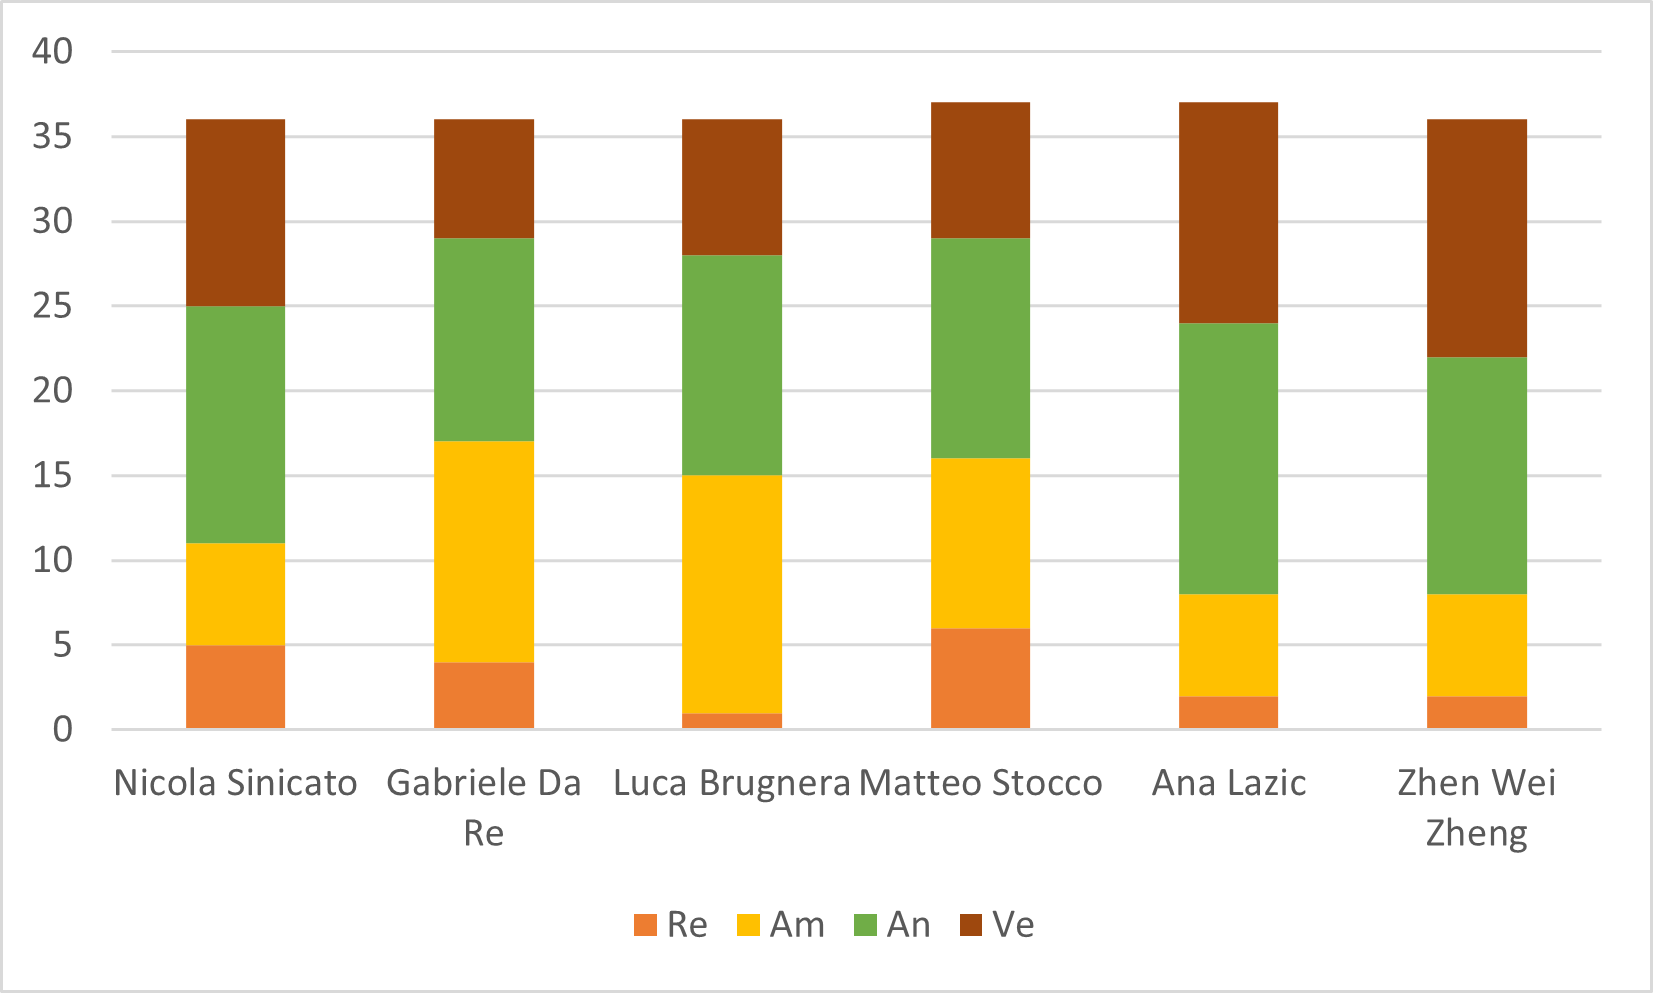
\includegraphics[scale=0.6]{img/grafi preventivo/istogrammi/analisi/complessivo.png}
    \caption{Istogramma della ripartizione delle ore della fase di analisi}
\end{figure}
\begin{figure}[H]
    \centering
    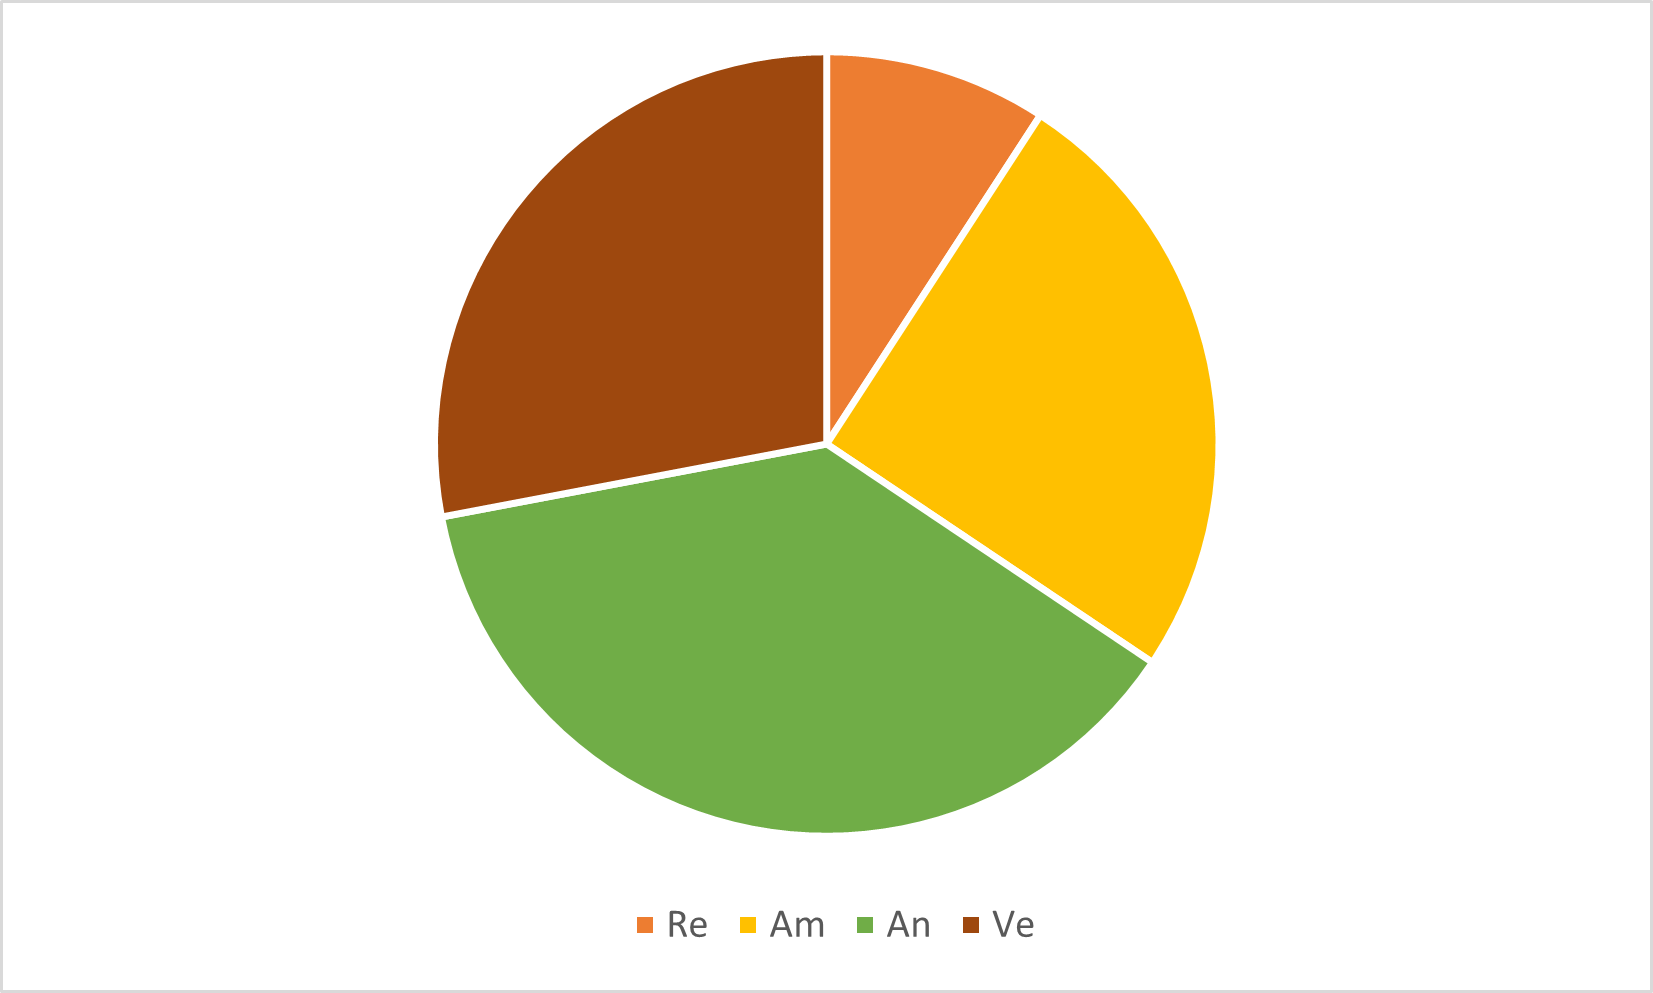
\includegraphics[scale=0.6]{img/grafi preventivo/torta/analisi/complessivo.png}
    \caption{Grafico a torta della ripartizione delle ore per ruolo nella fase di analisi}
\end{figure}
\subsubsubsection{Preventivo dei costi}
La seguente tabella rappresenta le ore dedicate ad ogni ruolo e il corrispettivo costo in euro per la fase di analisi:

	\setlength\extrarowheight{5pt}
	\rowcolors{2}{gray!10}{gray!40}
	\begin{tabularx}{\textwidth}{|ccc|c|}
		\hline
		\rowcolor{white}
		\textbf{Ruolo} & \textbf{Costo orario (€)} & \textbf{Ore totali} & \textbf{Costo totale (€)} \\
		\hline
		Responsabile &30&15&450 \\
		Amministratore &20&47&940 \\
		Analista &25&80&2000 \\
		Verificatore &15&38&570 \\
		Programmatore &15&0&0 \\
		Progettista &25&0&0 \\
		\hline
		Totale &-&-&3960 \\
		\hline
		\rowcolor{white}
		\caption{Prospetto del costo orario durante la fase di analisi per ruolo}
	\end{tabularx}
    \vspace{10pt}
	
% ----------------------------------------------------------------------------------------------------------------
%
\newpage
\subsection{Produzione del Proof of Concept}

% ----------------------------------------------------------------------------------------------------------------
\subsubsection{Periodo 1}
% ----------------------------------------------------------------------------------------------------------------
%
\subsubsubsection{Preventivo orario}
La seguente tabella rappresenta la distribuzione oraria per ogni componente per il primo periodo della fase di produzione del Proof of Concept:

	\setlength\extrarowheight{5pt}
	\rowcolors{2}{gray!10}{gray!40}
	\begin{tabularx}{\textwidth}{|ccccccc|c|}
		\hline
		\rowcolor{white}
		\textbf{Nome} & \textbf{Re} & \textbf{Am} & \textbf{An} & \textbf{Ve} & \textbf{Pr}& \textbf{Pt} & \textbf{Ore totali} \\
		\hline
		Nicola Sinicato &1&1&0&0&1&1&4 \\
		Gabriele Da Re &0&1&0&0&1&2&4 \\
		Luca Brugnera &1&0&1&1&0&1&4 \\
		Matteo Stocco &0&0&1&1&1&1&4 \\
		Ana Lazic &1&0&1&0&1&1&4 \\
		Zhen Wei Zheng &1&1&1&0&0&1&4 \\
		\hline
		Ore totali ruolo &4&3&4&2&4&7&24 \\
		\hline
		\rowcolor{white}
		\caption{Distribuzione oraria durante  il primo periodo di produzione del Proof of Concept per ruolo e persona}
	\end{tabularx}
	\vspace{10pt}
	
\begin{figure}[H]
    \centering
    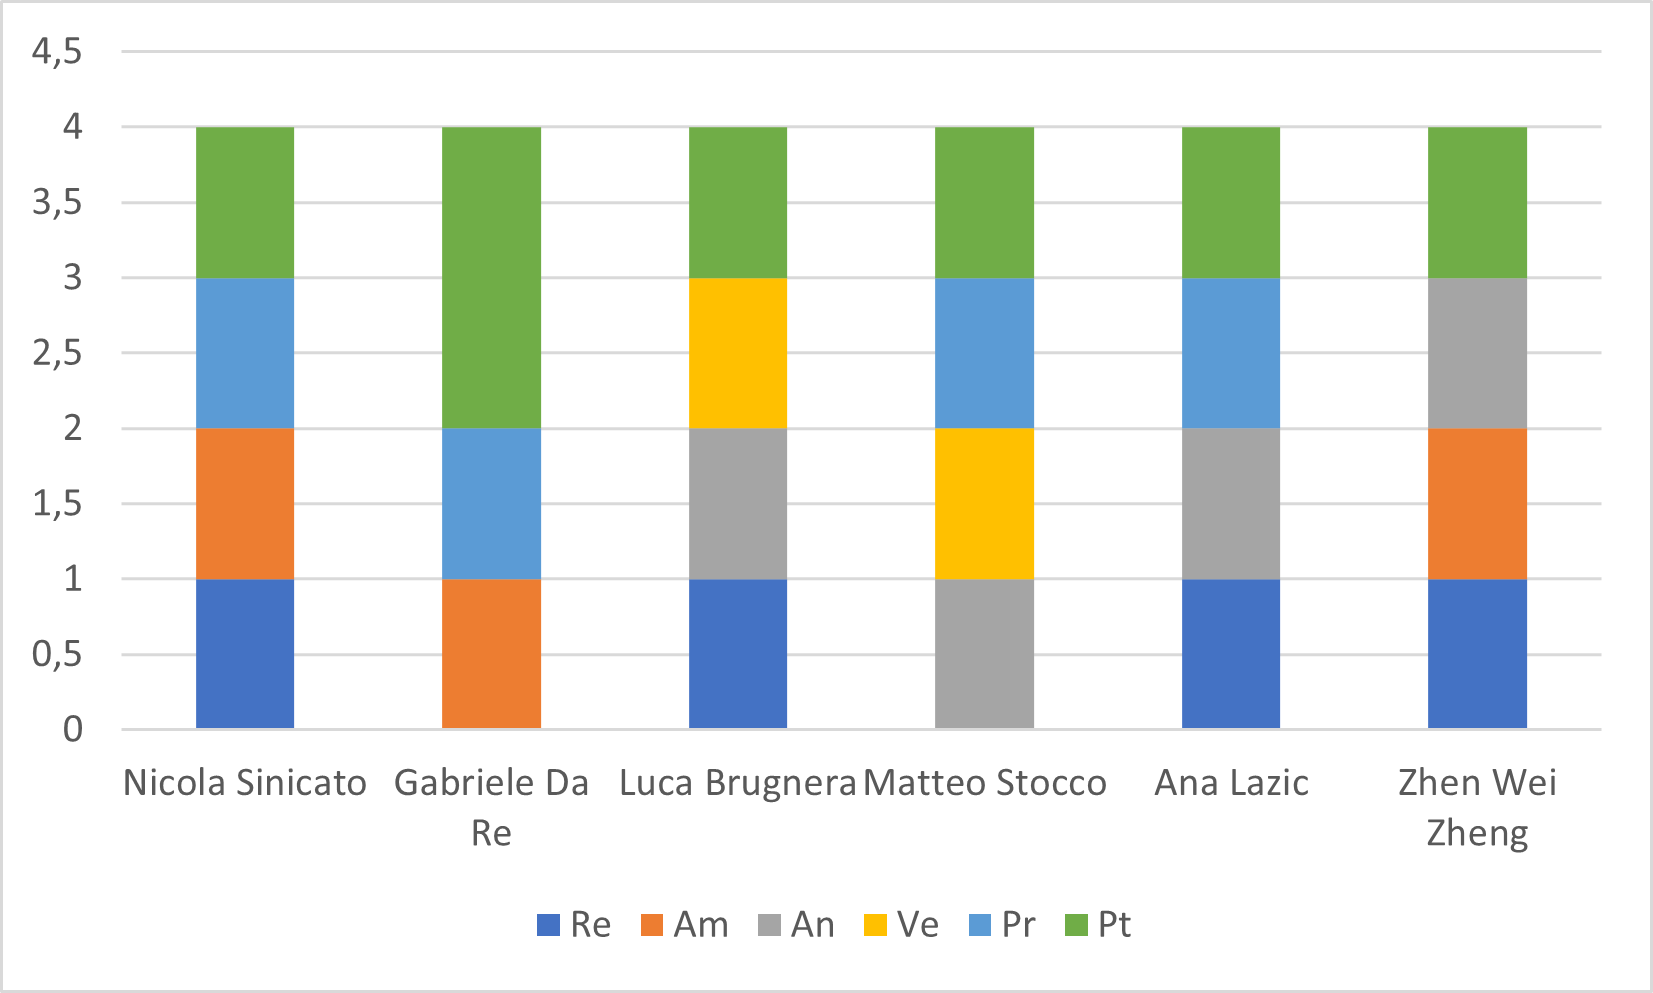
\includegraphics[scale=0.6]{img/grafi preventivo/istogrammi/proof/periodo1.png}
    \caption{Istogramma della ripartizione delle ore del primo periodo della fase di produzione del Proof of Concept}
\end{figure}
\begin{figure}[H]
    \centering
    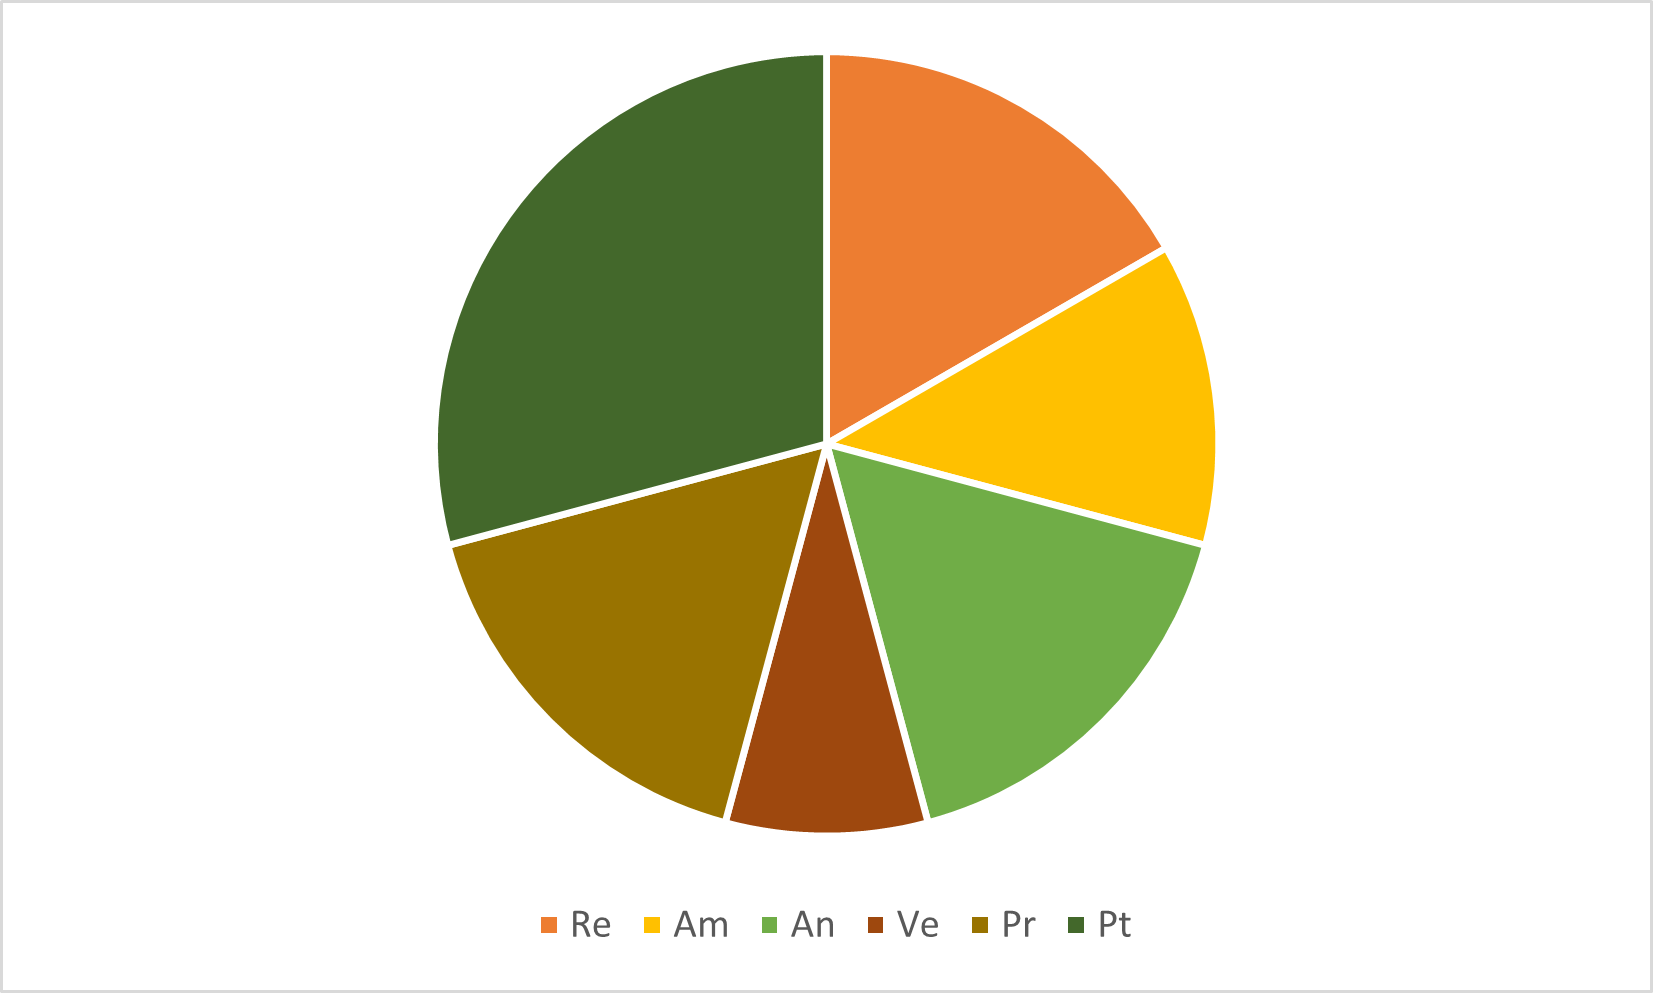
\includegraphics[scale=0.6]{img/grafi preventivo/torta/proof/periodo1.png}
    \caption{Grafico a torta della ripartizione delle ore per ruolo nel primo periodo della fase di produzione del Proof of Concept}
\end{figure}
\subsubsubsection{Preventivo dei costi}
La seguente tabella rappresenta le ore dedicate ad ogni ruolo e il corrispettivo costo in euro per il primo periodo della fase di produzione del Proof of Concept:

	\setlength\extrarowheight{5pt}
	\rowcolors{2}{gray!10}{gray!40}
	\begin{tabularx}{\textwidth}{|ccc|c|}
		\hline
		\rowcolor{white}
		\textbf{Ruolo} & \textbf{Costo orario (€)} & \textbf{Ore totali} & \textbf{Costo totale (€)} \\
		\hline
		Responsabile &30&4&120 \\
		Amministratore &20&3&60 \\
		Analista &25&4&100 \\
		Verificatore &15&2&30 \\
		Programmatore &15&4&60 \\
		Progettista &25&7&175 \\
		\hline
		Totale &-&-&545 \\
		\hline
		\rowcolor{white}
		\caption{Prospetto del costo orario durante  il primo periodo di produzione del Proof of Concept per ruolo}
	\end{tabularx}
    \vspace{10pt}
	
% ----------------------------------------------------------------------------------------------------------------
\newpage
\subsubsection{Periodo 2}
% ----------------------------------------------------------------------------------------------------------------
%
\subsubsubsection{Preventivo orario}
La seguente tabella rappresenta la distribuzione oraria per ogni componente per il secondo periodo della fase di produzione del Proof of Concept:

	\setlength\extrarowheight{5pt}
	\rowcolors{2}{gray!10}{gray!40}
	\begin{tabularx}{\textwidth}{|ccccccc|c|}
		\hline
		\rowcolor{white}
		\textbf{Nome} & \textbf{Re} & \textbf{Am} & \textbf{An} & \textbf{Ve} & \textbf{Pr}& \textbf{Pt} & \textbf{Ore totali} \\
		\hline
		Nicola Sinicato &0&1&0&1&4&0&6 \\
		Gabriele Da Re &2&0&0&0&0&4&6 \\
		Luca Brugnera &0&0&2&1&3&0&6 \\
		Matteo Stocco &0&1&0&4&1&0&6 \\
		Ana Lazic &0&1&2&0&3&0&6 \\
		Zhen Wei Zheng &1&0&0&2&0&3&6 \\
		\hline
		Ore totali ruolo &3&3&4&8&11&7&36 \\
		\hline
		\rowcolor{white}
		\caption{Distribuzione oraria durante il secondo periodo di produzione del Proof of Concept per ruolo e persona}
	\end{tabularx}
	\vspace{10pt}
	
\begin{figure}[H]
    \centering
    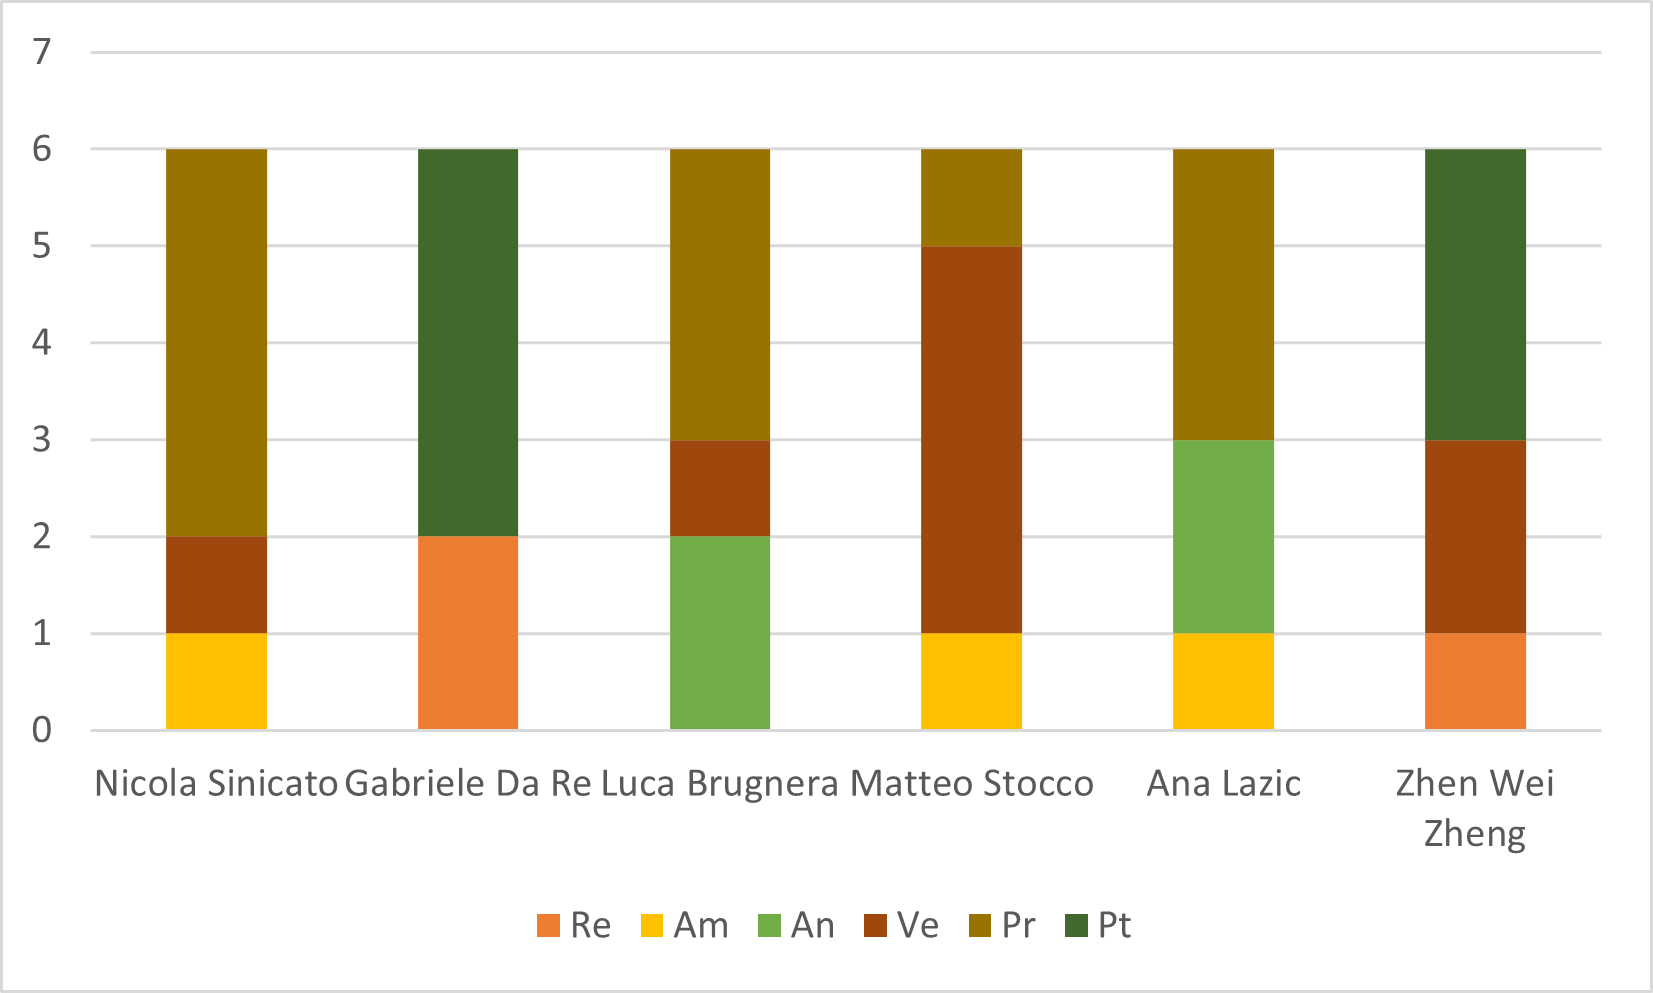
\includegraphics[scale=0.6]{img/grafi preventivo/istogrammi/proof/periodo2.png}
    \caption{Istogramma della ripartizione delle ore del secondo periodo della fase di produzione del Proof of Concept}
\end{figure}
\begin{figure}[H]
    \centering
    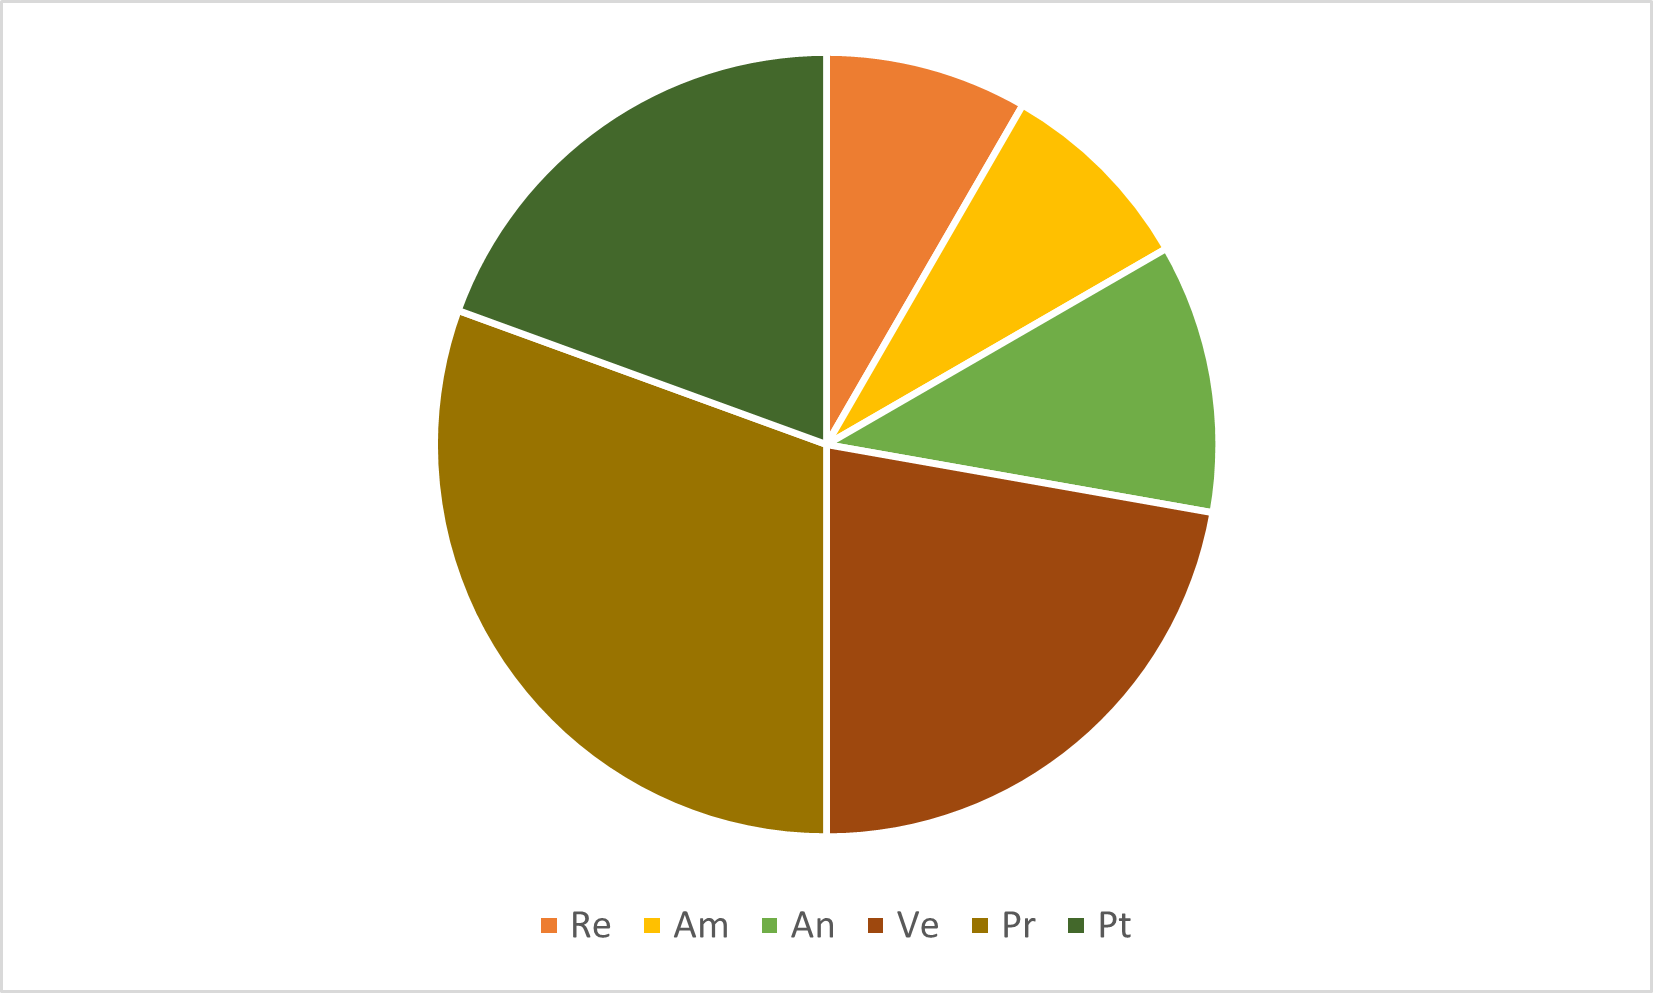
\includegraphics[scale=0.6]{img/grafi preventivo/torta/proof/periodo2.png}
    \caption{Grafico a torta della ripartizione delle ore per ruolo nel secondo periodo della fase di produzione del Proof of Concept}
\end{figure}
\subsubsubsection{Preventivo dei costi}
La seguente tabella rappresenta le ore dedicate ad ogni ruolo e il corrispettivo costo in euro per il secondo periodo della fase di produzione del Proof of Concept:

	\setlength\extrarowheight{5pt}
	\rowcolors{2}{gray!10}{gray!40}
	\begin{tabularx}{\textwidth}{|ccc|c|}
		\hline
		\rowcolor{white}
		\textbf{Ruolo} & \textbf{Costo orario (€)} & \textbf{Ore totali} & \textbf{Costo totale (€)} \\
		\hline
		Responsabile &30&3&90 \\
		Amministratore &20&3&60 \\
		Analista &25&4&100 \\
		Verificatore &15&8&120 \\
		Programmatore &15&11&165 \\
		Progettista &25&7&175 \\
		\hline
		Totale &-&-&710 \\
		\hline
		\rowcolor{white}
		\caption{Prospetto del costo orario durante  il secondo periodo di produzione del Proof of Concept per ruolo}
	\end{tabularx}
    \vspace{10pt}
	
% ----------------------------------------------------------------------------------------------------------------
\newpage
\subsubsection{Riepilogo della fase di produzione del Proof of Concept}
% ----------------------------------------------------------------------------------------------------------------
%
\subsubsubsection{Preventivo orario}
La seguente tabella rappresenta la distribuzione oraria per ogni componente la fase di produzione del Proof of Concept:

	\setlength\extrarowheight{5pt}
	\rowcolors{2}{gray!10}{gray!40}
	\begin{tabularx}{\textwidth}{|ccccccc|c|}
		\hline
		\rowcolor{white}
		\textbf{Nome} & \textbf{Re} & \textbf{Am} & \textbf{An} & \textbf{Ve} & \textbf{Pr}& \textbf{Pt} & \textbf{Ore totali} \\
		\hline
		Nicola Sinicato &1&2&0&1&5&1&10 \\
		Gabriele Da Re &2&1&0&0&1&6&10 \\
		Luca Brugnera &1&0&3&2&3&1&10 \\
		Matteo Stocco &0&1&1&5&2&1&10 \\
		Ana Lazic &1&1&3&0&4&1&10 \\
		Zhen Wei Zheng &2&1&1&2&0&4&10 \\
		\hline
		Ore totali ruolo &7&6&8&10&15&14&60 \\
		\hline
		\rowcolor{white}
		\caption{Distribuzione oraria durante la fase di produzione del Proof of Concept per ruolo e persona}
	\end{tabularx}
	\vspace{10pt}
	
\begin{figure}[H]
    \centering
    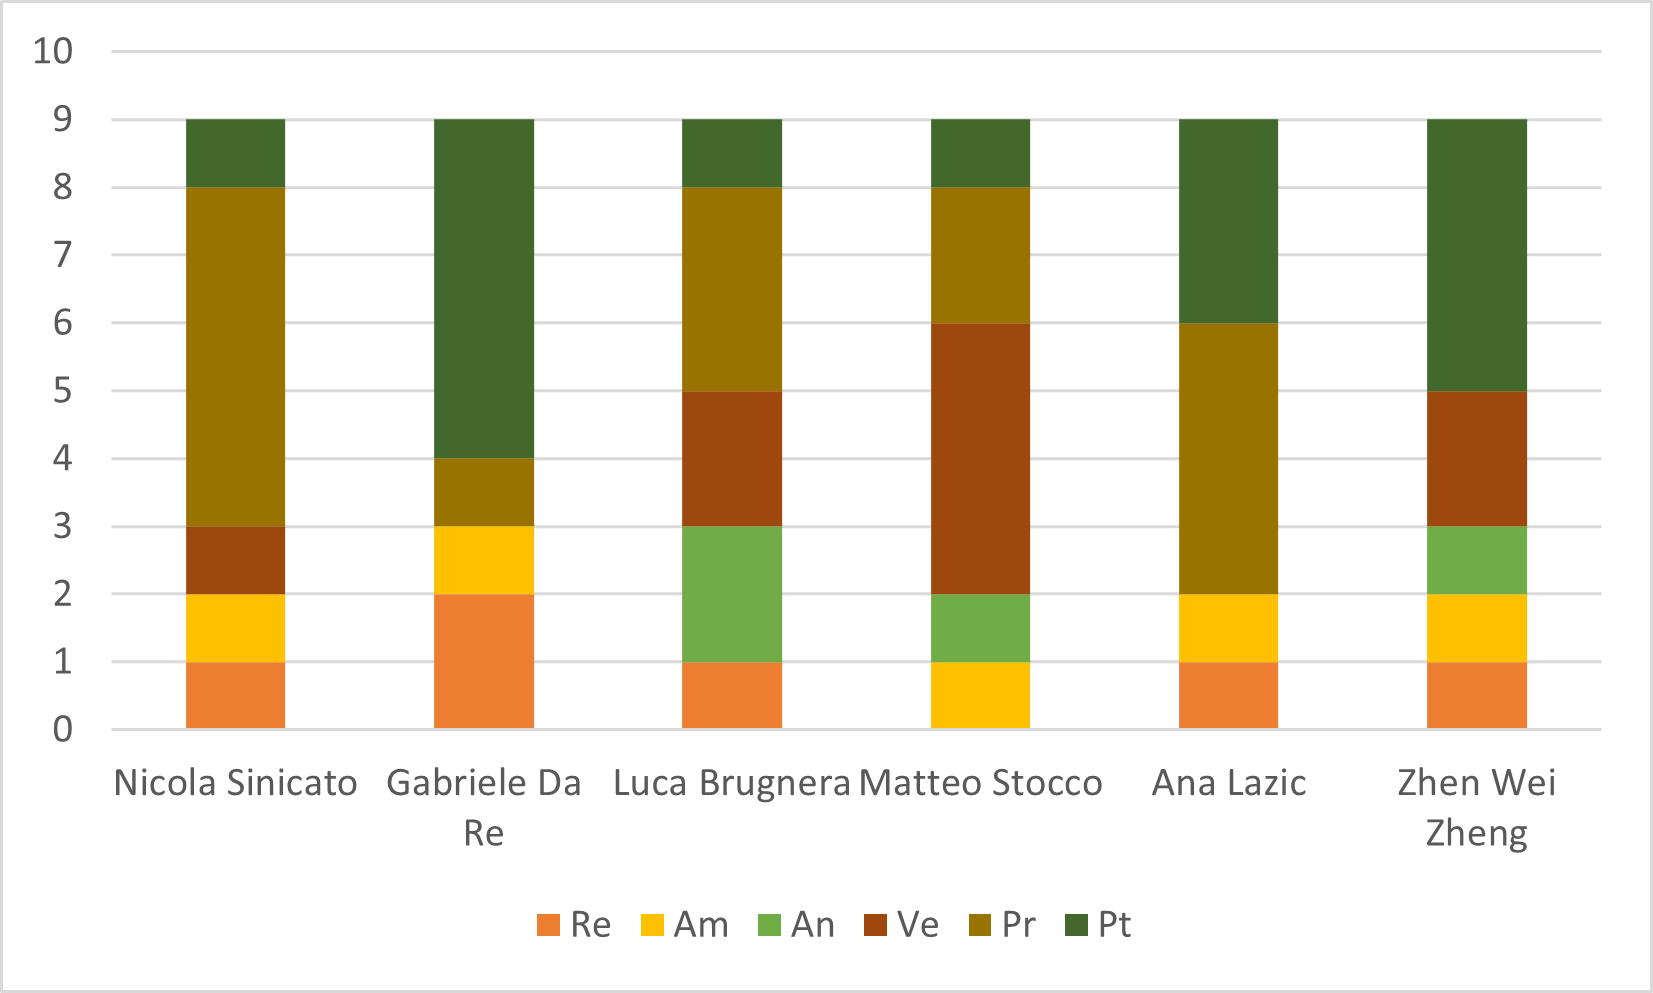
\includegraphics[scale=0.6]{img/grafi preventivo/istogrammi/proof/complessivo.png}
    \caption{Istogramma della ripartizione delle ore della fase di produzione del Proof of Concept}
\end{figure}
\begin{figure}[H]
    \centering
    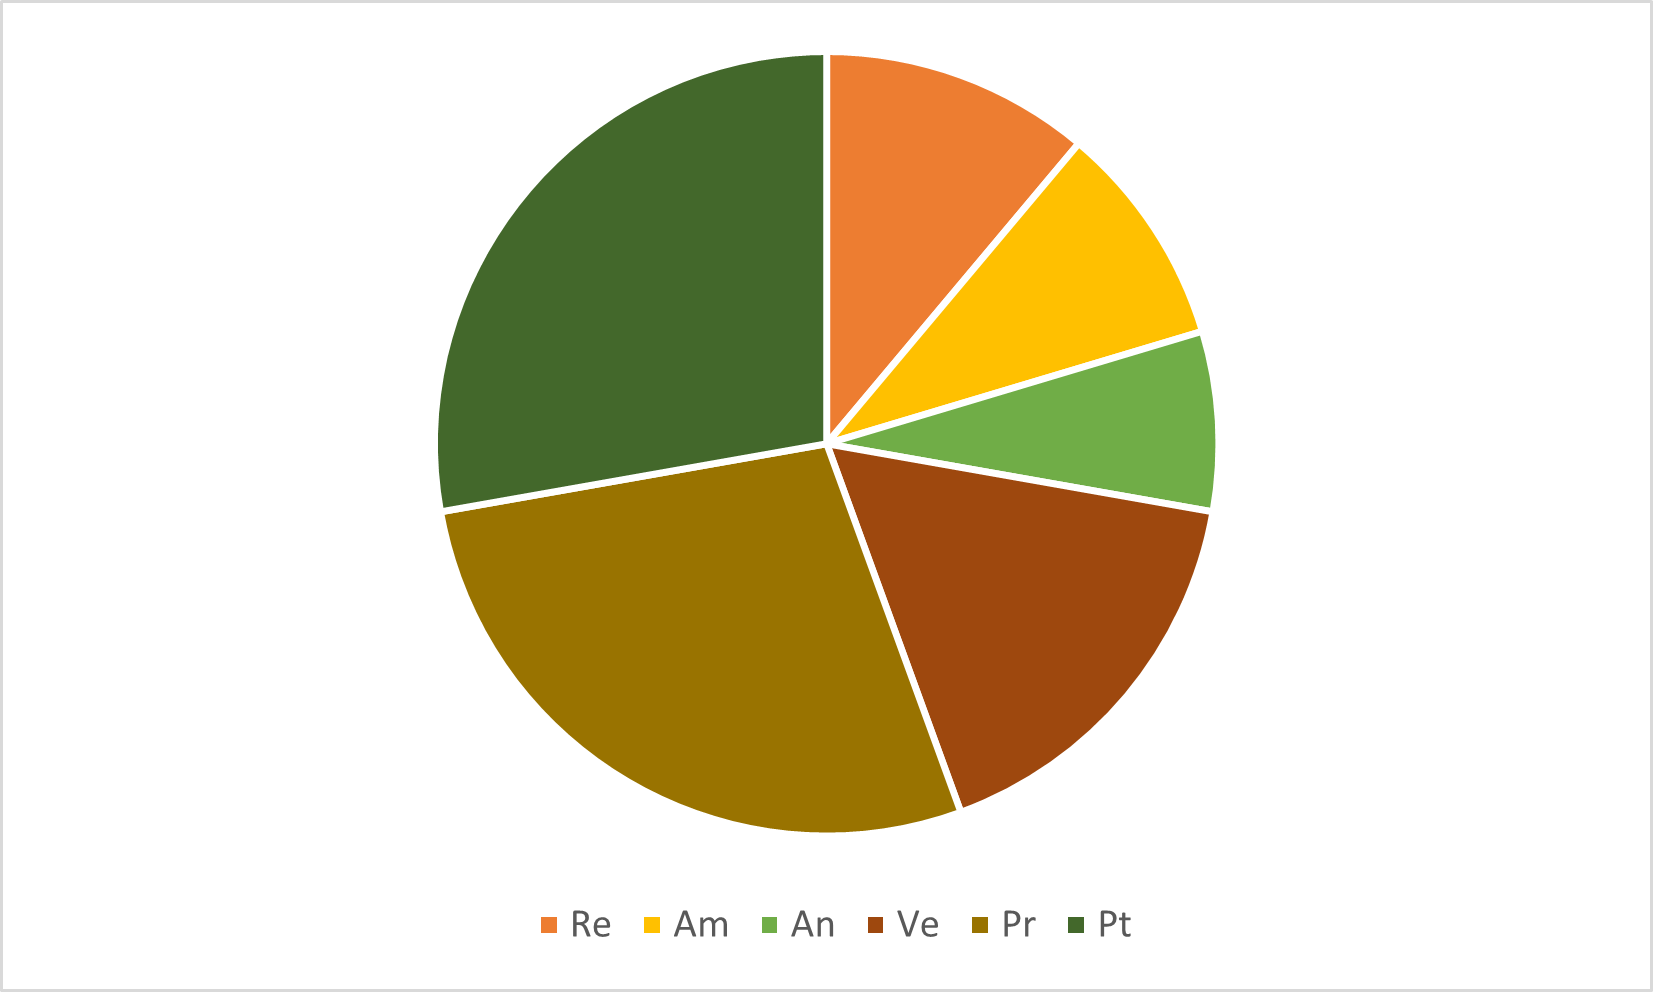
\includegraphics[scale=0.6]{img/grafi preventivo/torta/proof/complessivo.png}
    \caption{Grafico a torta della ripartizione delle ore per ruolo nella fase di produzione del Proof of Concept}
\end{figure}
\subsubsubsection{Preventivo dei costi}
La seguente tabella rappresenta le ore dedicate ad ogni ruolo e il corrispettivo costo in euro per la fase di produzione del Proof of Concept:

	\setlength\extrarowheight{5pt}
	\rowcolors{2}{gray!10}{gray!40}
	\begin{tabularx}{\textwidth}{|ccc|c|}
		\hline
		\rowcolor{white}
		\textbf{Ruolo} & \textbf{Costo orario (€)} & \textbf{Ore totali} & \textbf{Costo totale (€)} \\
		\hline
		Responsabile &30&7&210 \\
		Amministratore &20&6&120 \\
		Analista &25&8&200 \\
		Verificatore &15&10&150 \\
		Programmatore &15&15&225 \\
		Progettista &25&14&350 \\
		\hline
		Totale &-&-&1255 \\
		\hline
		\rowcolor{white}
		\caption{Prospetto del costo orario durante la fase di produzione del Proof of Concept per ruolo}
	\end{tabularx}
    \vspace{10pt}
	
% ----------------------------------------------------------------------------------------------------------------
%
\newpage
\subsection{Progettazione architetturale}

% ----------------------------------------------------------------------------------------------------------------
\subsubsection{Periodo 1}
% ----------------------------------------------------------------------------------------------------------------
%
\subsubsubsection{Preventivo orario}
La seguente tabella rappresenta la distribuzione oraria per ogni componente per il primo periodo della fase di progettazione architetturale:

	\setlength\extrarowheight{5pt}
	\rowcolors{2}{gray!10}{gray!40}
	\begin{tabularx}{\textwidth}{|ccccccc|c|}
		\hline
		\rowcolor{white}
		\textbf{Nome} & \textbf{Re} & \textbf{Am} & \textbf{An} & \textbf{Ve} & \textbf{Pr}& \textbf{Pt} & \textbf{Ore totali} \\
		\hline
		Nicola Sinicato &1&0&2&0&0&1&4 \\
		Gabriele Da Re &0&0&1&2&0&1&4 \\
		Luca Brugnera &1&0&3&0&0&0&4 \\
		Matteo Stocco &0&1&0&2&0&1&4 \\
		Ana Lazic &0&0&2&0&0&2&4 \\
		Zhen Wei Zheng &1&0&0&1&0&2&4 \\
		\hline
		Ore totali ruolo &3&1&8&5&0&7&24 \\
		\hline
		\rowcolor{white}
		\caption{Distribuzione oraria durante  il primo periodo di progettazione architetturale per ruolo e persona}
	\end{tabularx}
	\vspace{10pt}
	
\begin{figure}[H]
    \centering
    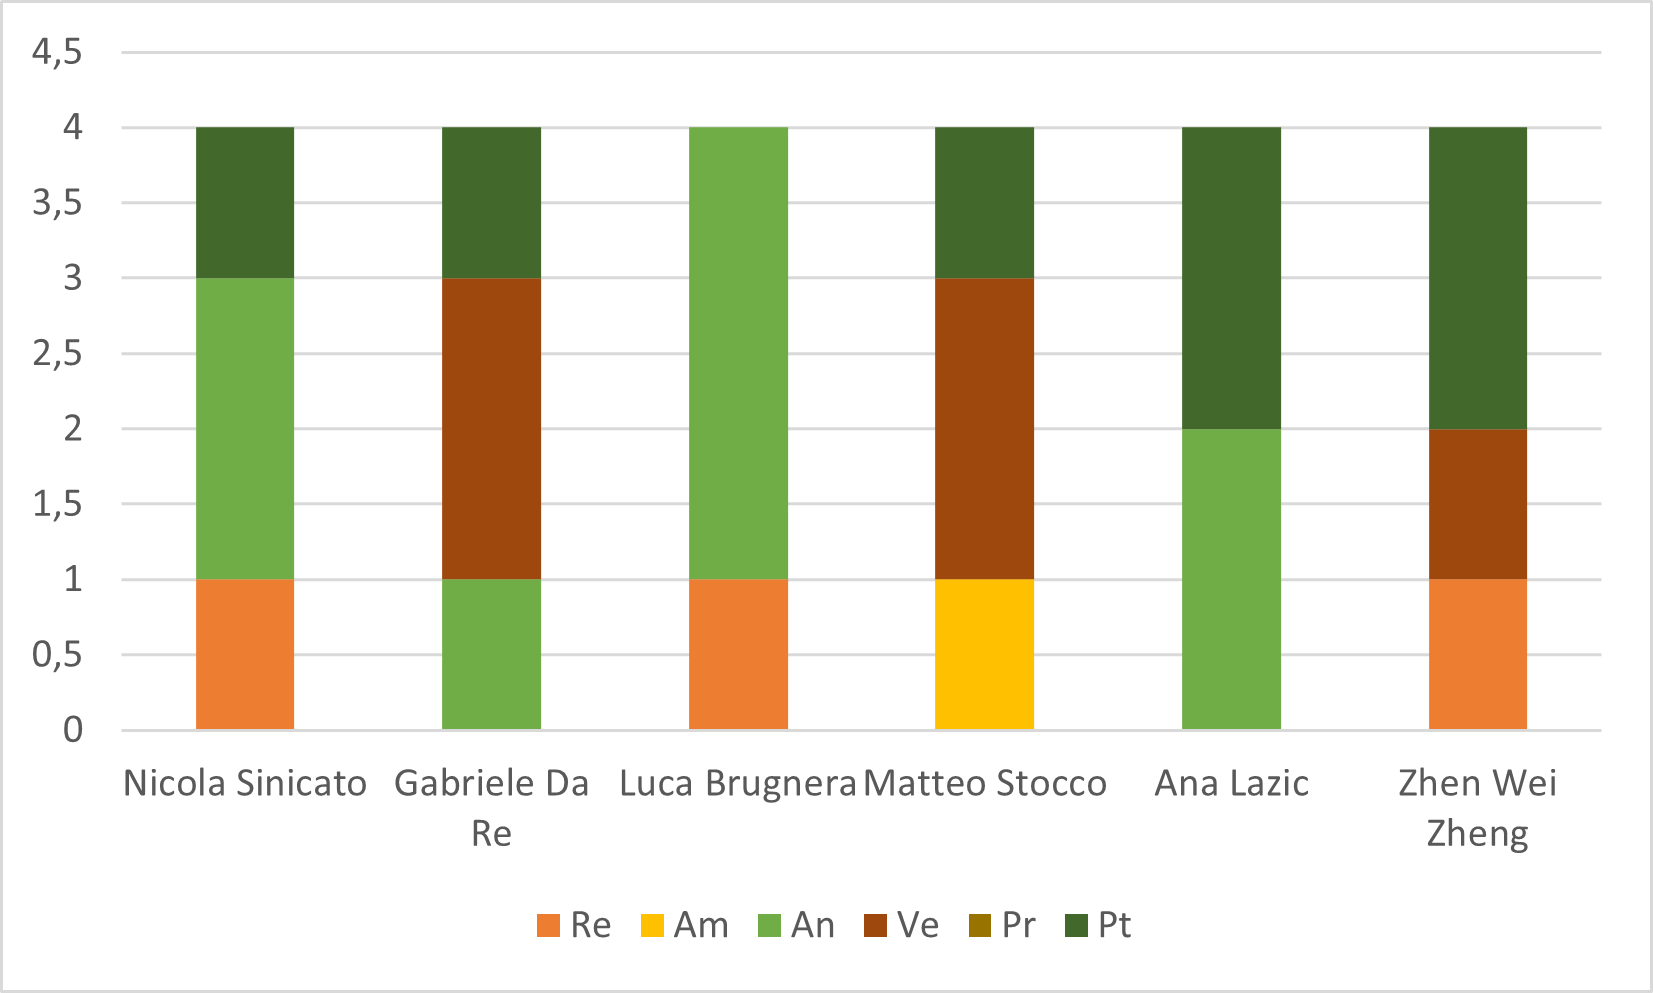
\includegraphics[scale=0.6]{img/grafi preventivo/istogrammi/architetturale/periodo1.png}
    \caption{Istogramma della ripartizione delle ore del primo periodo della fase di progettazione architetturale}
\end{figure}
\begin{figure}[H]
    \centering
    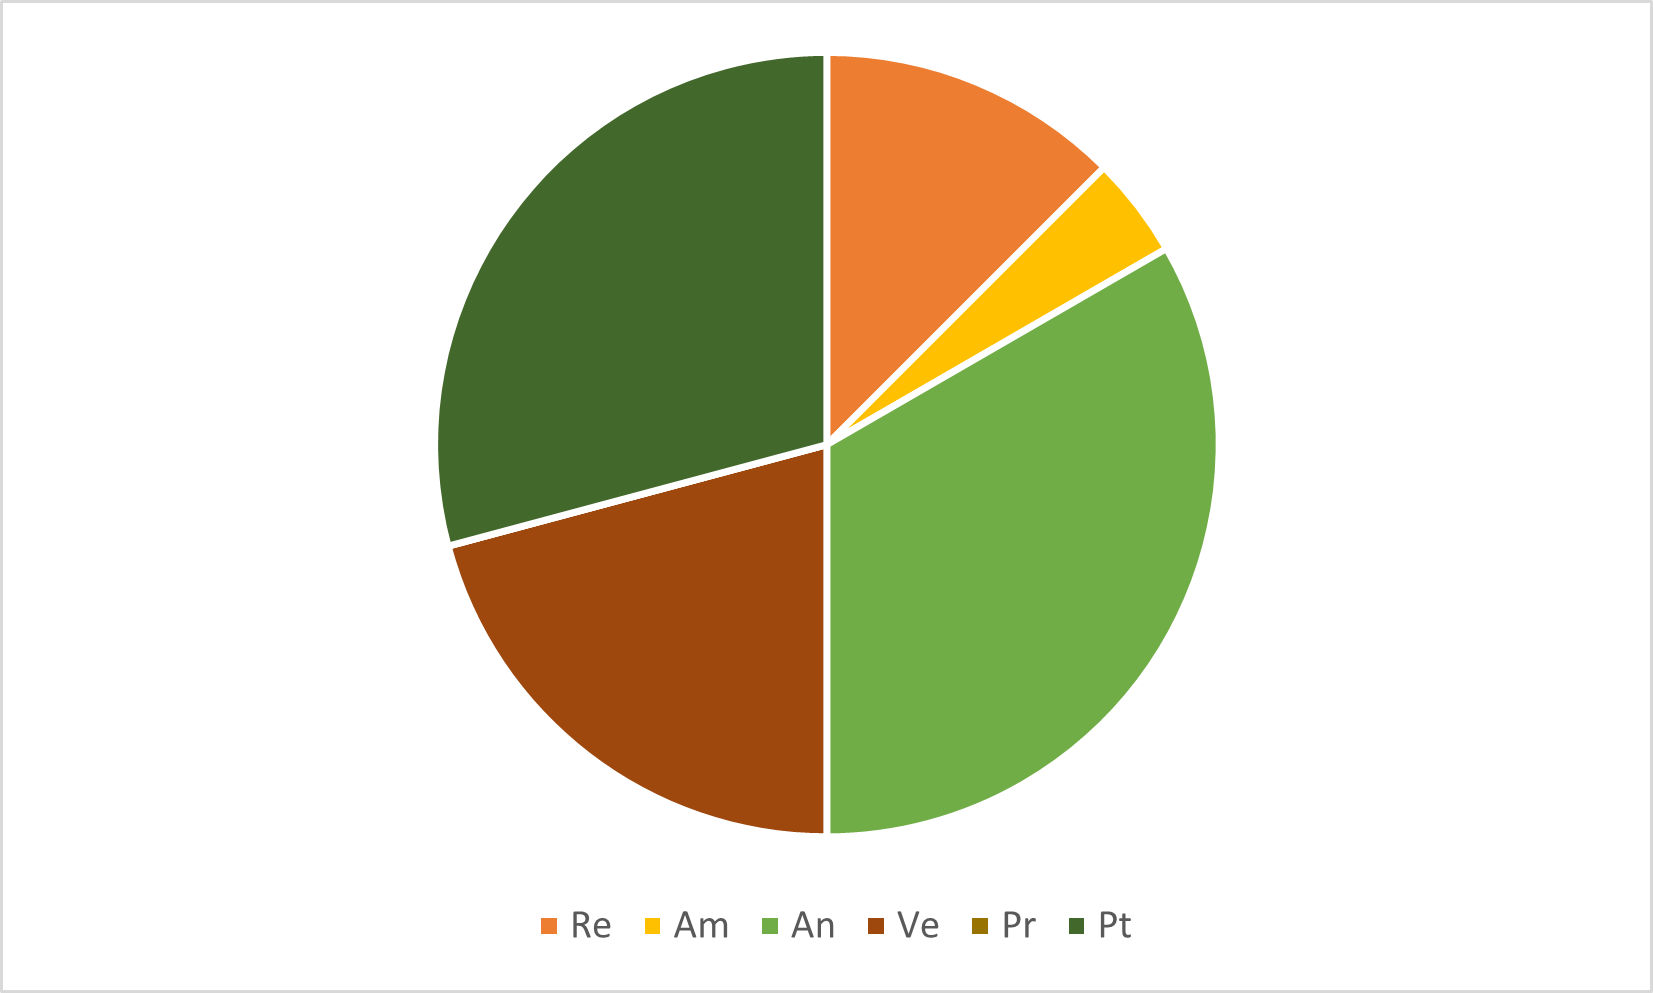
\includegraphics[scale=0.6]{img/grafi preventivo/torta/architetturale/periodo1.png}
    \caption{Grafico a torta della ripartizione delle ore per ruolo nel primo periodo della fase di progettazione architetturale}
\end{figure}
\subsubsubsection{Preventivo dei costi}
La seguente tabella rappresenta le ore dedicate ad ogni ruolo e il corrispettivo costo in euro per il primo periodo della fase di progettazione architetturale:

	\setlength\extrarowheight{5pt}
	\rowcolors{2}{gray!10}{gray!40}
	\begin{tabularx}{\textwidth}{|ccc|c|}
		\hline
		\rowcolor{white}
		\textbf{Ruolo} & \textbf{Costo orario (€)} & \textbf{Ore totali} & \textbf{Costo totale (€)} \\
		\hline
		Responsabile &30&3&90 \\
		Amministratore &20&1&20 \\
		Analista &25&8&200 \\
		Verificatore &15&5&75 \\
		Programmatore &15&0&0 \\
		Progettista &25&7&175 \\
		\hline
		Totale &-&-&560 \\
		\hline
		\rowcolor{white}
		\caption{Prospetto del costo orario durante  il primo periodo di progettazione architetturale per ruolo}
	\end{tabularx}
    \vspace{10pt}
	
% ----------------------------------------------------------------------------------------------------------------
\newpage
\subsubsection{Periodo 2}
% ----------------------------------------------------------------------------------------------------------------
%
\subsubsubsection{Preventivo orario}
La seguente tabella rappresenta la distribuzione oraria per ogni componente per il secondo periodo di fase di progettazione architetturale:

	\setlength\extrarowheight{5pt}
	\rowcolors{2}{gray!10}{gray!40}
	\begin{tabularx}{\textwidth}{|ccccccc|c|}
		\hline
		\rowcolor{white}
		\textbf{Nome} & \textbf{Re} & \textbf{Am} & \textbf{An} & \textbf{Ve} & \textbf{Pr}& \textbf{Pt} & \textbf{Ore totali} \\
		\hline
		Nicola Sinicato &0&1&0&0&0&8&9 \\
		Gabriele Da Re &1&1&0&2&0&5&9 \\
		Luca Brugnera &0&1&0&0&0&8&9 \\
		Matteo Stocco &1&0&0&1&0&7&9 \\
		Ana Lazic &1&0&0&0&0&8&9 \\
		Zhen Wei Zheng &0&1&0&0&0&8&9 \\
		\hline
		Ore totali ruolo &3&4&0&3&0&44&54 \\
		\hline
		\rowcolor{white}
		\caption{Distribuzione oraria durante il secondo periodo di progettazione architetturale per ruolo e persona}
	\end{tabularx}
	\vspace{10pt}
	
\begin{figure}[H]
    \centering
    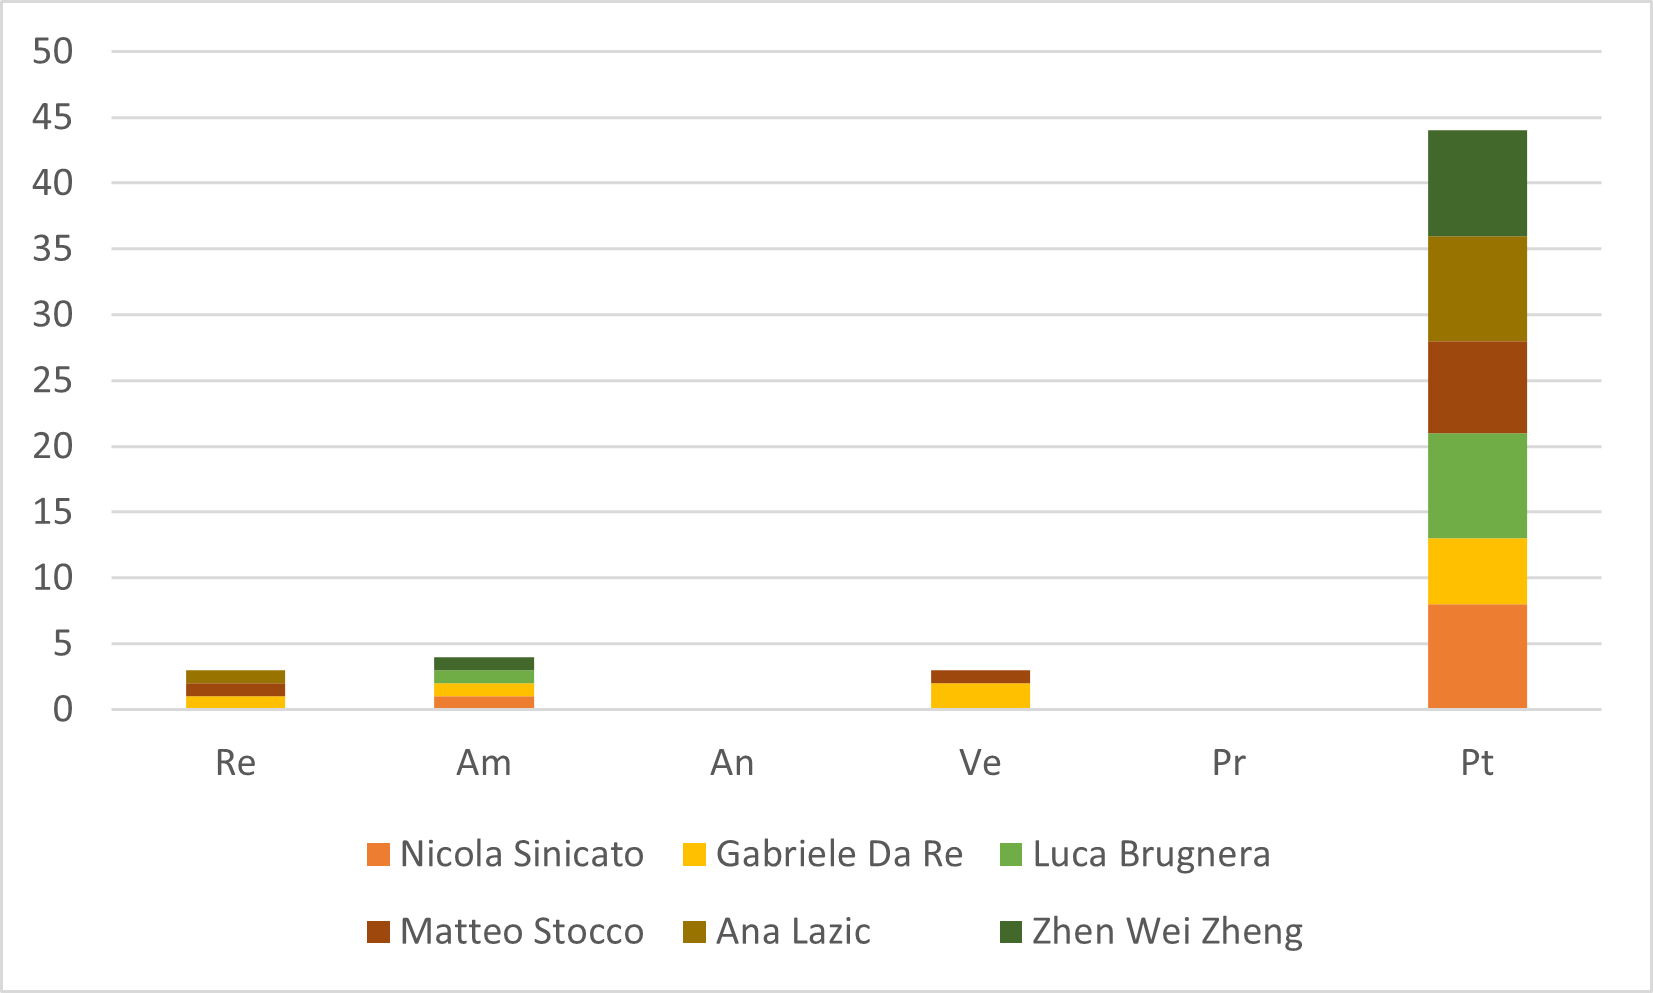
\includegraphics[scale=0.6]{img/grafi preventivo/istogrammi/architetturale/periodo2.png}
    \caption{Istogramma della ripartizione delle ore del secondo periodo della fase di progettazione architetturale}
\end{figure}
\begin{figure}[H]
    \centering
    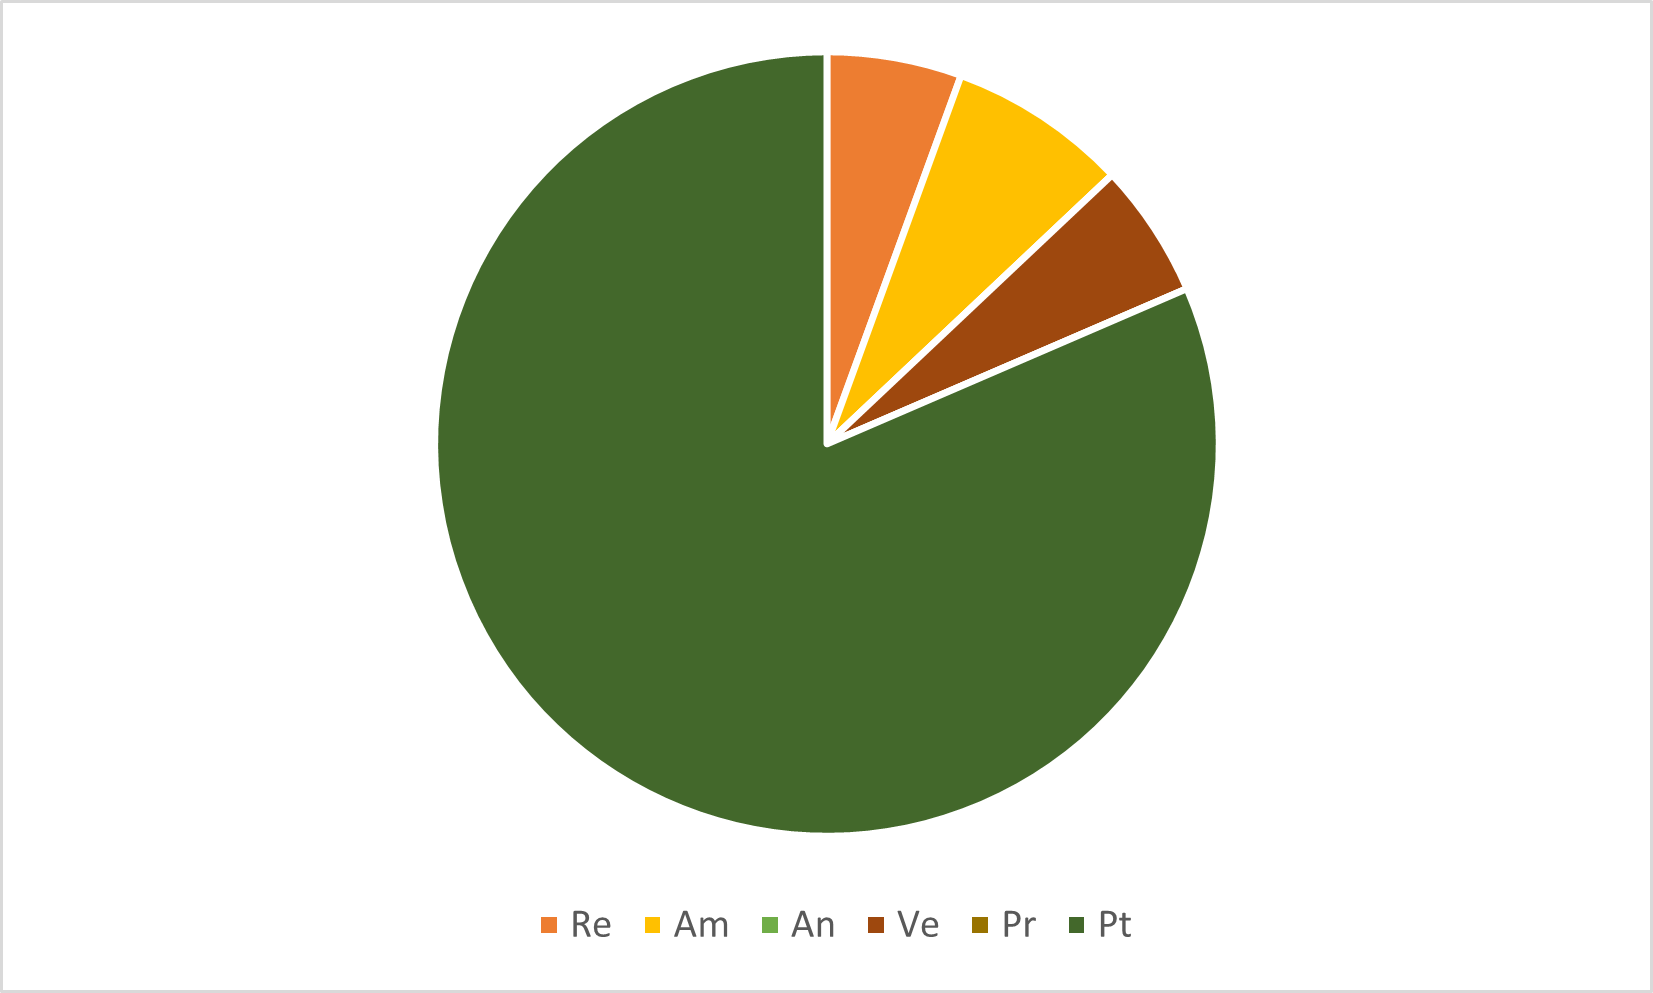
\includegraphics[scale=0.6]{img/grafi preventivo/torta/architetturale/periodo2.png}
    \caption{Grafico a torta della ripartizione delle ore per ruolo nel secondo periodo della fase di progettazione architetturale}
\end{figure}
\subsubsubsection{Preventivo dei costi}
La seguente tabella rappresenta le ore dedicate ad ogni ruolo e il corrispettivo costo in euro per il secondo periodo della fase di progettazione architetturale:

	\setlength\extrarowheight{5pt}
	\rowcolors{2}{gray!10}{gray!40}
	\begin{tabularx}{\textwidth}{|ccc|c|}
		\hline
		\rowcolor{white}
		\textbf{Ruolo} & \textbf{Costo orario (€)} & \textbf{Ore totali} & \textbf{Costo totale (€)} \\
		\hline
		Responsabile &30&3&90 \\
		Amministratore &20&4&80 \\
		Analista &25&0&0 \\
		Verificatore &15&3&45 \\
		Programmatore &15&0&0 \\
		Progettista &25&44&1100 \\
		\hline
		Totale &-&-&1315 \\
		\hline
		\rowcolor{white}
		\caption{Prospetto del costo orario durante il secondo periodo di progettazione architetturale per ruolo}
	\end{tabularx}
    \vspace{10pt}
	
% ----------------------------------------------------------------------------------------------------------------
\newpage
\subsubsection{Riepilogo della fase di progettazione architetturale }
% ----------------------------------------------------------------------------------------------------------------
%
\subsubsubsection{Preventivo orario}
La seguente tabella rappresenta la distribuzione oraria per ogni componente per la fase di progettazione architetturale:

	\setlength\extrarowheight{5pt}
	\rowcolors{2}{gray!10}{gray!40}
	\begin{tabularx}{\textwidth}{|ccccccc|c|}
		\hline
		\rowcolor{white}
		\textbf{Nome} & \textbf{Re} & \textbf{Am} & \textbf{An} & \textbf{Ve} & \textbf{Pr}& \textbf{Pt} & \textbf{Ore totali} \\
		\hline
		Nicola Sinicato &1&1&2&0&0&9&13 \\
		Gabriele Da Re &1&1&1&4&0&6&13 \\
		Luca Brugnera &1&1&3&0&0&8&13 \\
		Matteo Stocco &1&1&0&3&0&8&13 \\
		Ana Lazic &1&0&2&0&0&10&13 \\
		Zhen Wei Zheng &1&1&0&1&0&10&13 \\
		\hline
		Ore totali ruolo &6&5&8&8&0&51&78 \\
		\hline
		\rowcolor{white}
		\caption{Distribuzione oraria durante la fase di progettazione architetturale per ruolo e persona}
	\end{tabularx}
	\vspace{10pt}
	
\begin{figure}[H]
    \centering
    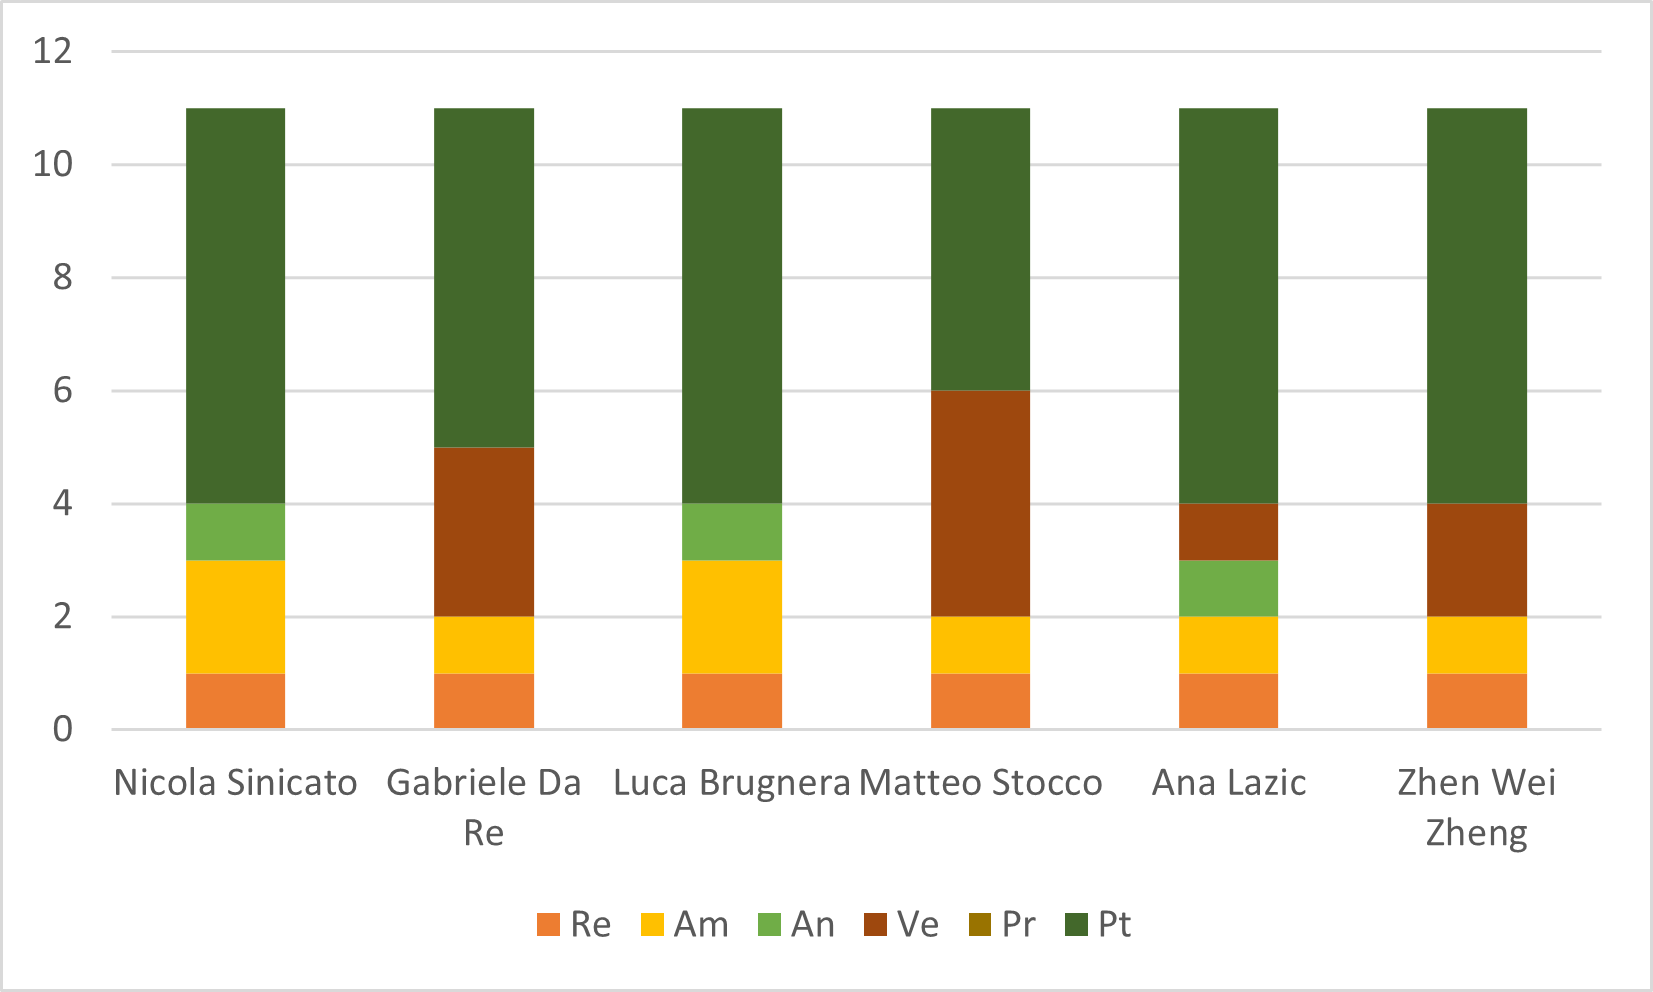
\includegraphics[scale=0.6]{img/grafi preventivo/istogrammi/architetturale/complessivo.png}
    \caption{Istogramma della ripartizione delle ore della fase di progettazione architetturale}
\end{figure}
\begin{figure}[H]
    \centering
    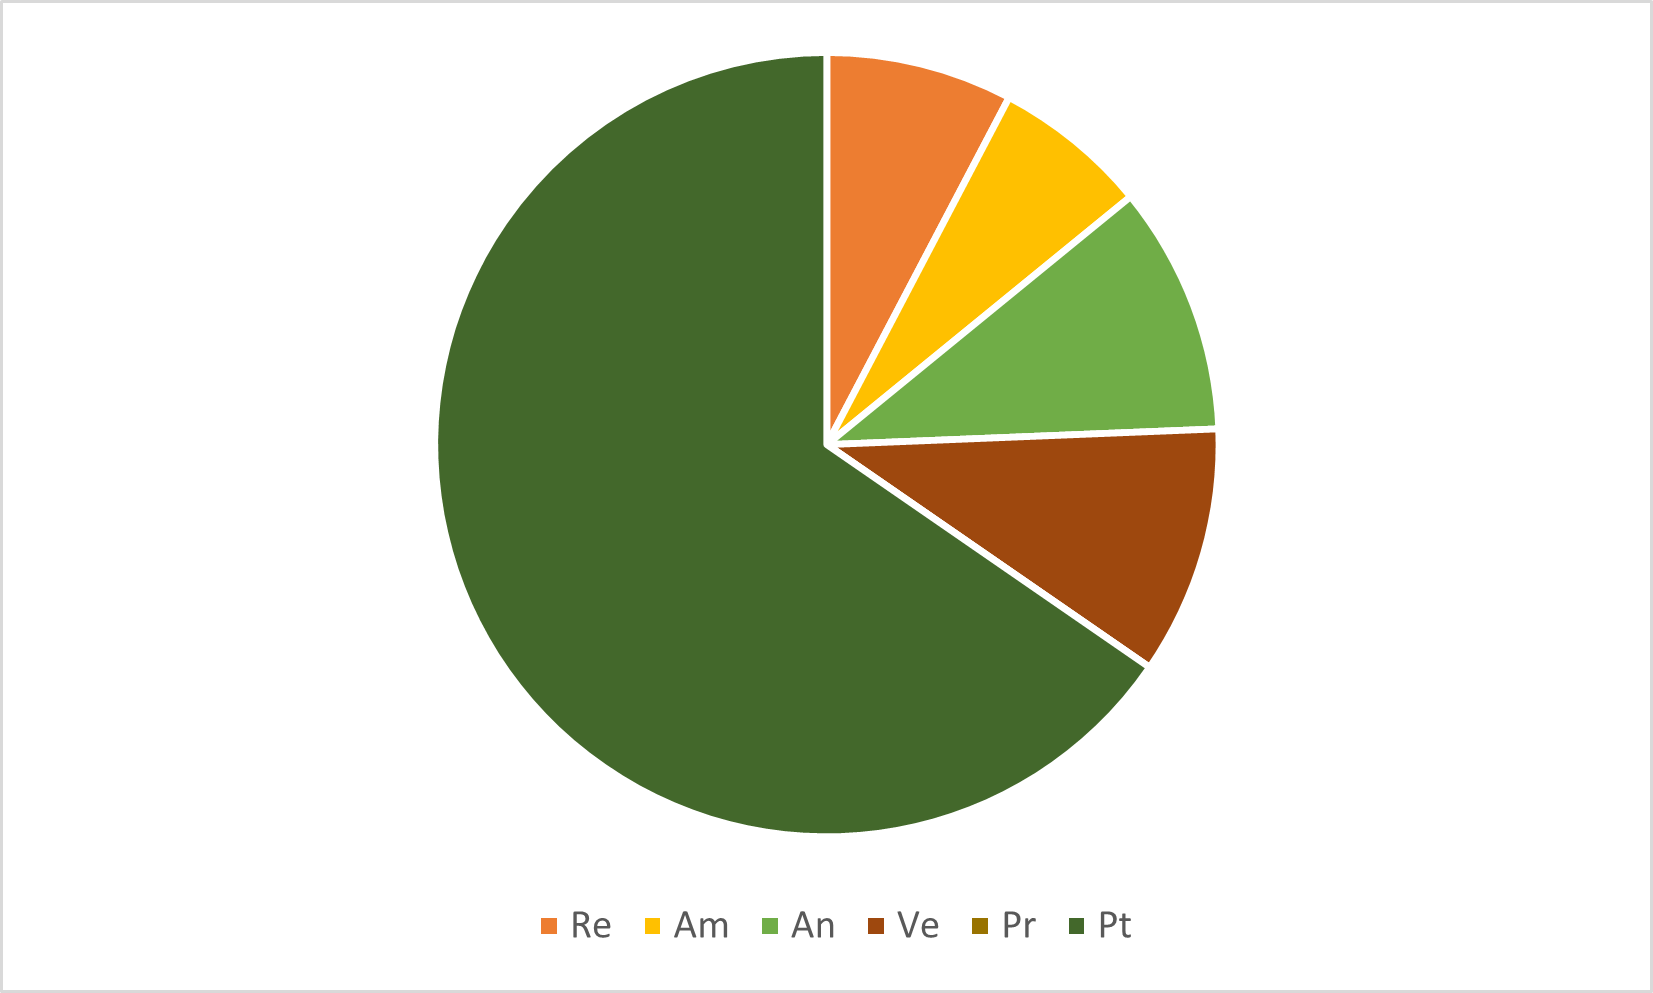
\includegraphics[scale=0.6]{img/grafi preventivo/torta/architetturale/complessivo.png}
    \caption{Grafico a torta della ripartizione delle ore per ruolo nella fase di progettazione architetturale}
\end{figure}
\subsubsubsection{Preventivo dei costi}
La seguente tabella rappresenta le ore dedicate ad ogni ruolo e il corrispettivo costo in euro per la fase di progettazione architetturale:

	\setlength\extrarowheight{5pt}
	\rowcolors{2}{gray!10}{gray!40}
	\begin{tabularx}{\textwidth}{|ccc|c|}
		\hline
		\rowcolor{white}
		\textbf{Ruolo} & \textbf{Costo orario (€)} & \textbf{Ore totali} & \textbf{Costo totale (€)} \\
		\hline
		Responsabile &30&6&180 \\
		Amministratore &20&5&100 \\
		Analista &25&8&200 \\
		Verificatore &15&8&120 \\
		Programmatore &15&0&0 \\
		Progettista &25&51&1275 \\
		\hline
		Totale &-&-&1875 \\
		\hline
		\rowcolor{white}
		\caption{Prospetto del costo orario durante la fase di progettazione architetturale per ruolo}
	\end{tabularx}
    \vspace{10pt}
	

% ----------------------------------------------------------------------------------------------------------------
\newpage
\subsection{Progettazione di dettaglio e codifica}
% ----------------------------------------------------------------------------------------------------------------
\subsubsection{Periodo 1}
% ----------------------------------------------------------------------------------------------------------------
%
\subsubsubsection{Preventivo orario}
La seguente tabella rappresenta la distribuzione oraria per ogni componente per il primo periodo di fase di progettazione di dettaglio e codifica:

	\setlength\extrarowheight{5pt}
	\rowcolors{2}{gray!10}{gray!40}
	\begin{tabularx}{\textwidth}{|ccccccc|c|}
		\hline
		\rowcolor{white}
		\textbf{Nome} & \textbf{Re} & \textbf{Am} & \textbf{An} & \textbf{Ve} & \textbf{Pr}& \textbf{Pt} & \textbf{Ore totali} \\
		\hline
		Nicola Sinicato &1&0&2&0&0&0&3 \\
		Gabriele Da Re &0&0&0&0&0&3&3 \\
		Luca Brugnera &0&1&0&2&0&0&3 \\
		Matteo Stocco &1&0&0&0&0&2&3 \\
		Ana Lazic &0&0&3&0&0&0&3 \\
		Zhen Wei Zheng &0&1&0&2&0&0&3 \\
		\hline
		Ore totali ruolo &2&2&5&4&0&5&18 \\
		\hline
		\rowcolor{white}
		\caption{Distribuzione oraria durante il primo periodo di progettazione di dettaglio e codifica per ruolo e persona}
	\end{tabularx}
	\vspace{10pt}
	
\begin{figure}[H]
    \centering
    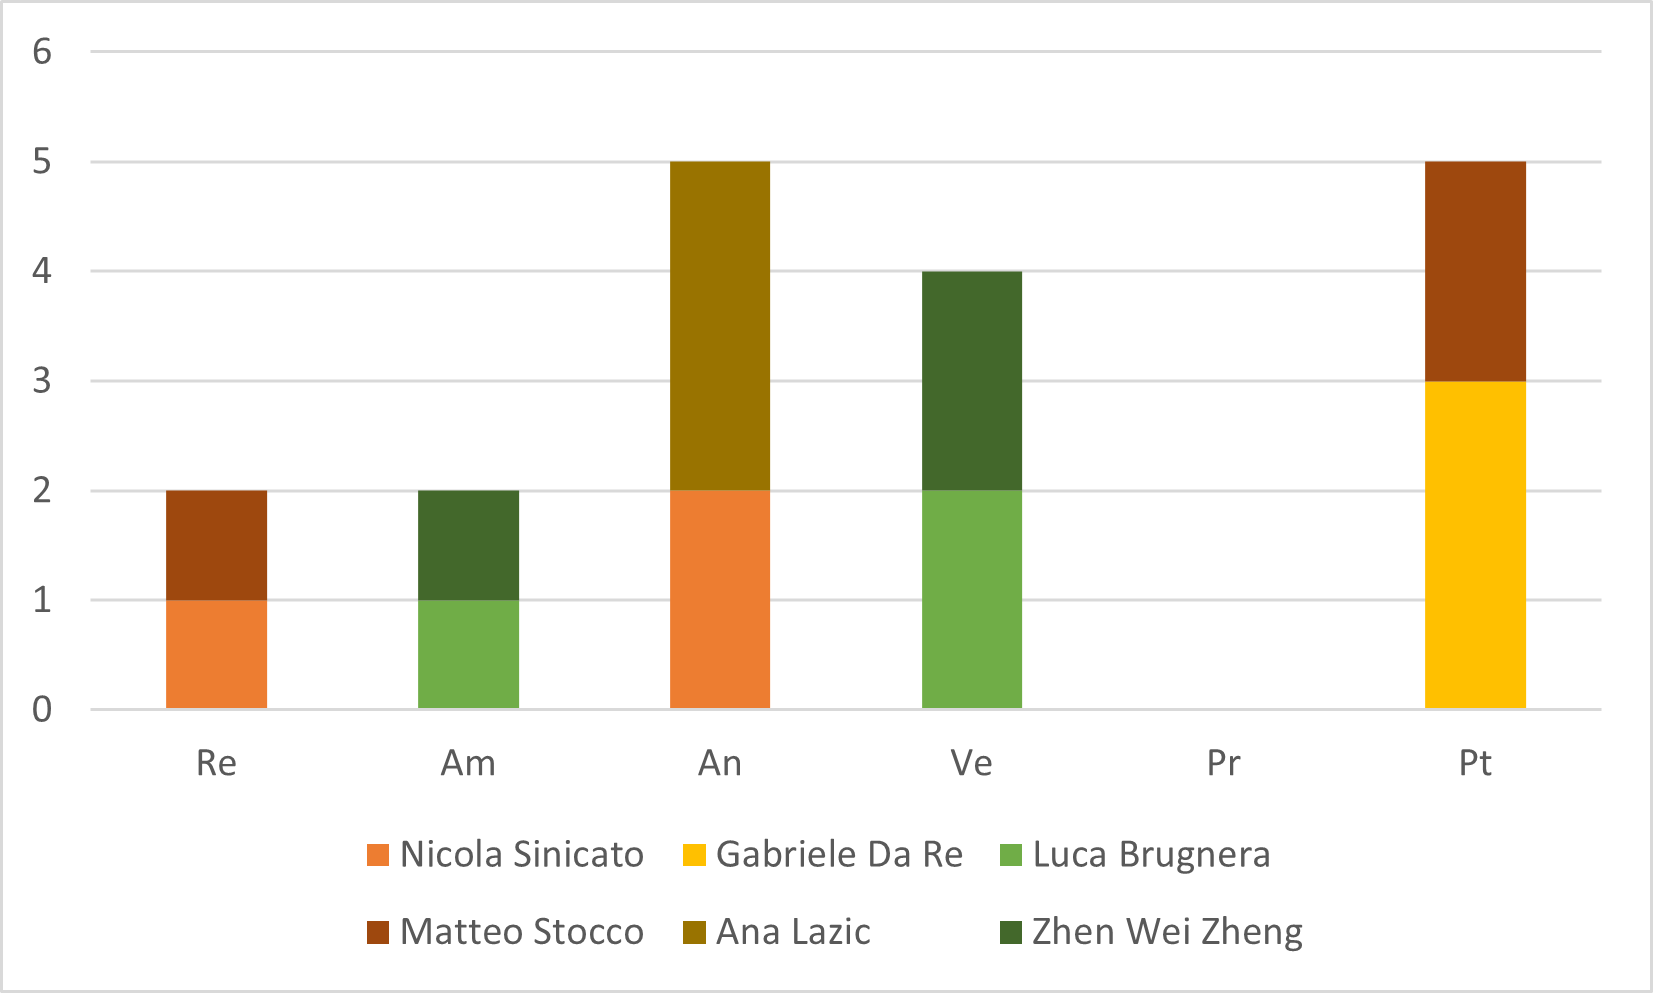
\includegraphics[scale=0.6]{img/grafi preventivo/istogrammi/codifica/periodo1.png}
    \caption{Istogramma della ripartizione delle ore del primo periodo della fase di progettazione di dettaglio e codifica}
\end{figure}
\begin{figure}[H]
    \centering
    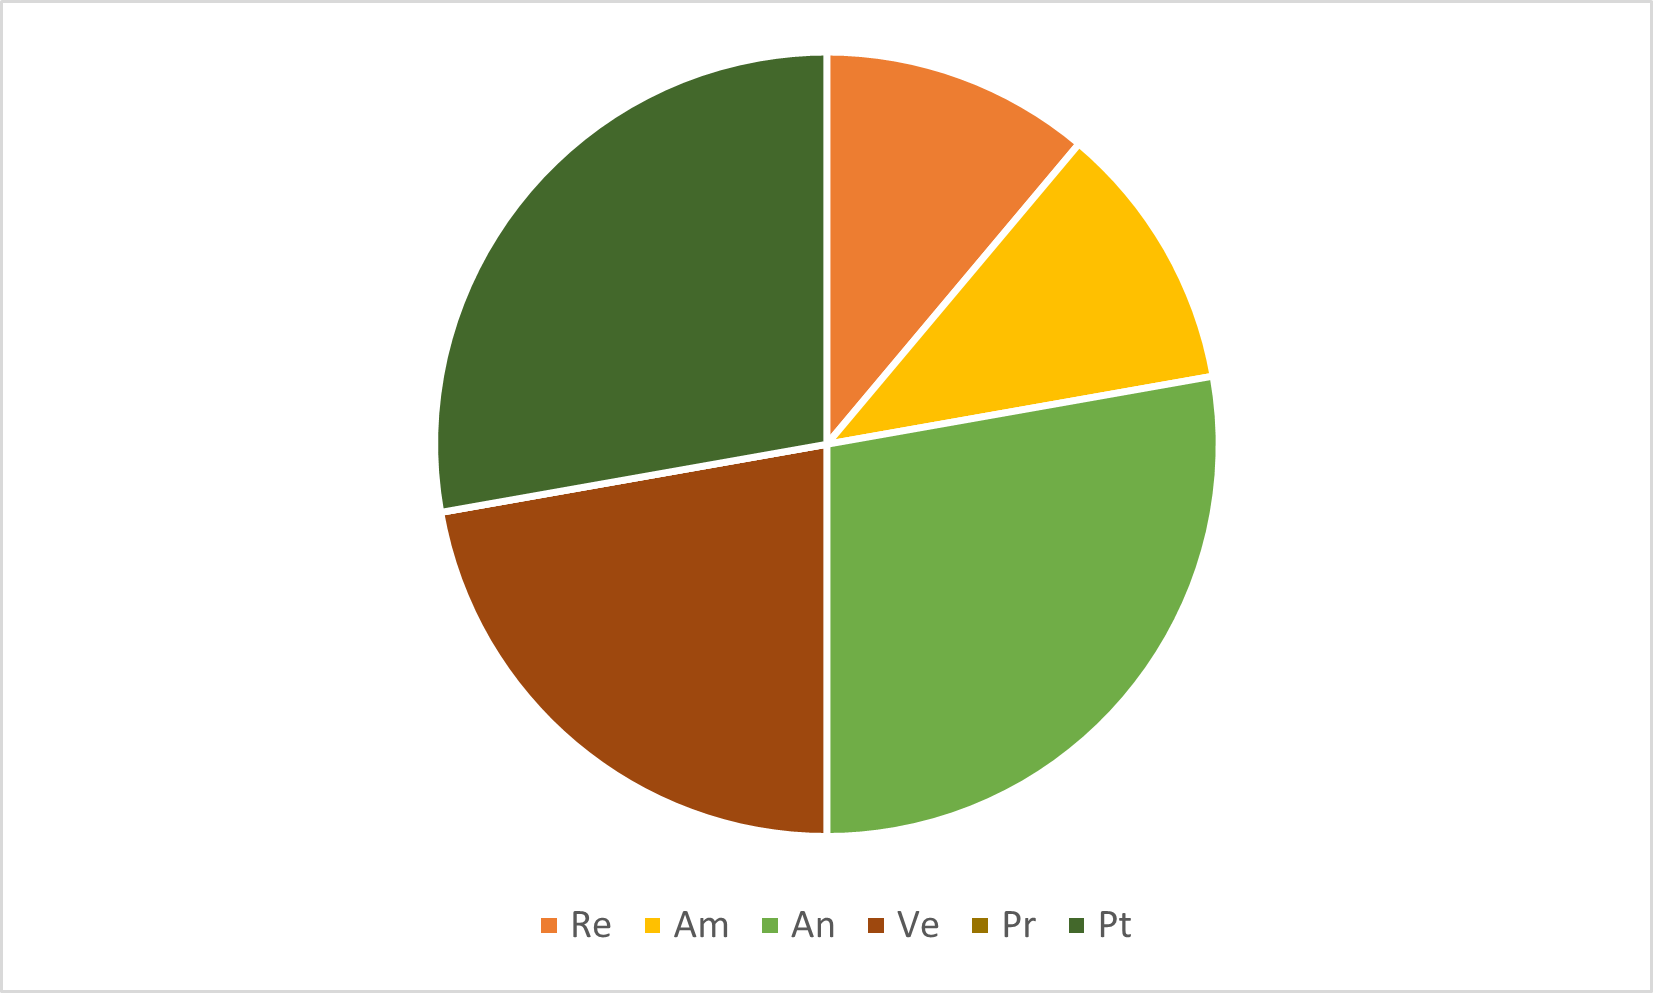
\includegraphics[scale=0.6]{img/grafi preventivo/torta/codifica/periodo1.png}
    \caption{Grafico a torta della ripartizione delle ore per ruolo nel primo periodo della fase di progettazione di dettaglio e codifica}
\end{figure}
\subsubsubsection{Preventivo dei costi}
La seguente tabella rappresenta le ore dedicate ad ogni ruolo e il corrispettivo costo in euro per il primo periodo della fase di progettazione di dettaglio e codifica:

	\setlength\extrarowheight{5pt}
	\rowcolors{2}{gray!10}{gray!40}
	\begin{tabularx}{\textwidth}{|ccc|c|}
		\hline
		\rowcolor{white}
		\textbf{Ruolo} & \textbf{Costo orario (€)} & \textbf{Ore totali} & \textbf{Costo totale (€)} \\
		\hline
		Responsabile &30&2&60 \\
		Amministratore &20&2&40 \\
		Analista &25&5&125 \\
		Verificatore &15&4&60 \\
		Programmatore &15&0&0 \\
		Progettista &25&5&125 \\
		\hline
		Totale &-&-&410 \\
		\hline
		\rowcolor{white}
		\caption{Prospetto del costo orario durante il primo periodo di progettazione di dettaglio e codifica per ruolo}
	\end{tabularx}
    \vspace{10pt}
	
%
% ----------------------------------------------------------------------------------------------------------------
\newpage
\subsubsection{Periodo 2}
% ----------------------------------------------------------------------------------------------------------------
%
\subsubsubsection{Preventivo orario}
La seguente tabella rappresenta la distribuzione oraria per ogni componente per il secondo periodo della fase di progettazione di dettaglio e codifica:

	\setlength\extrarowheight{5pt}
	\rowcolors{2}{gray!10}{gray!40}
	\begin{tabularx}{\textwidth}{|ccccccc|c|}
		\hline
		\rowcolor{white}
		\textbf{Nome} & \textbf{Re} & \textbf{Am} & \textbf{An} & \textbf{Ve} & \textbf{Pr}& \textbf{Pt} & \textbf{Ore totali} \\
		\hline
		Nicola Sinicato &0&0&0&2&14&0&16 \\
		Gabriele Da Re &0&1&0&1&11&3&16 \\
		Luca Brugnera &0&1&0&0&11&4&16 \\
		Matteo Stocco &0&0&0&2&14&0&16 \\
		Ana Lazic &1&0&0&2&11&2&16 \\
		Zhen Wei Zheng &1&2&0&2&11&0&16 \\
		\hline
		Ore totali ruolo &2&4&0&9&72&9&96 \\
		\hline
		\rowcolor{white}
		\caption{Distribuzione oraria durante  il secondo periodo di progettazione di dettaglio e codifica per ruolo e persona}
	\end{tabularx}
	\vspace{10pt}
	
\begin{figure}[H]
    \centering
    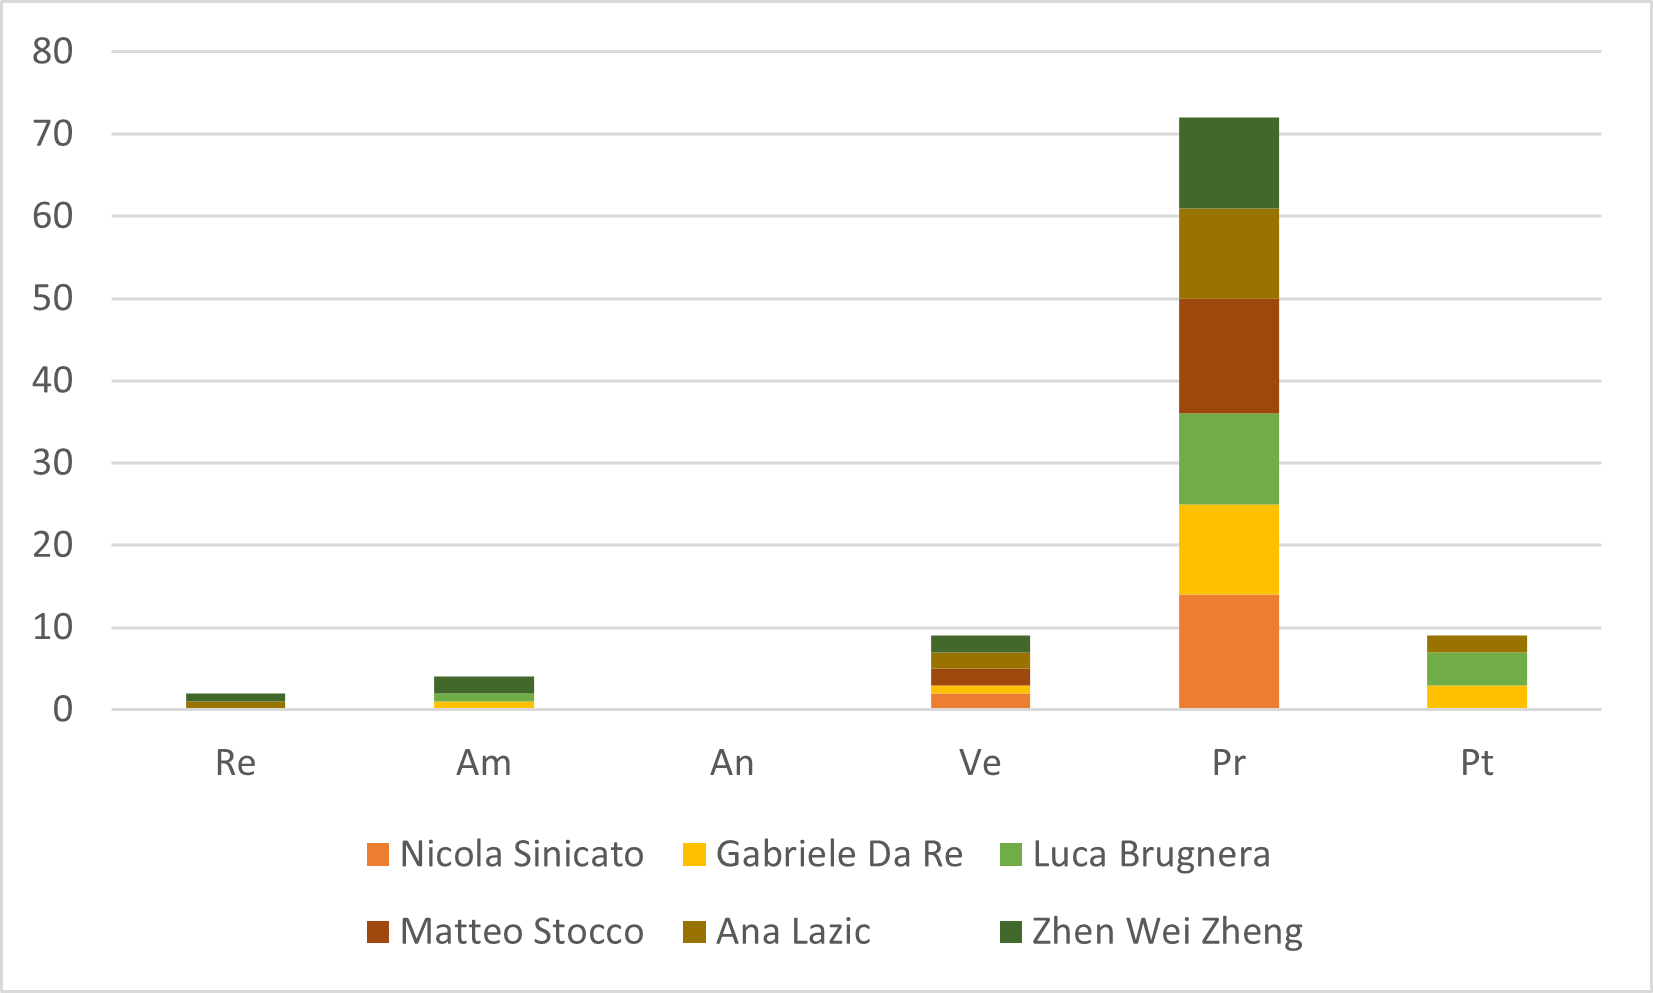
\includegraphics[scale=0.6]{img/grafi preventivo/istogrammi/codifica/periodo2.png}
    \caption{Istogramma della ripartizione delle ore del secondo periodo della fase di progettazione di dettaglio e codifica}
\end{figure}
\begin{figure}[H]
    \centering
    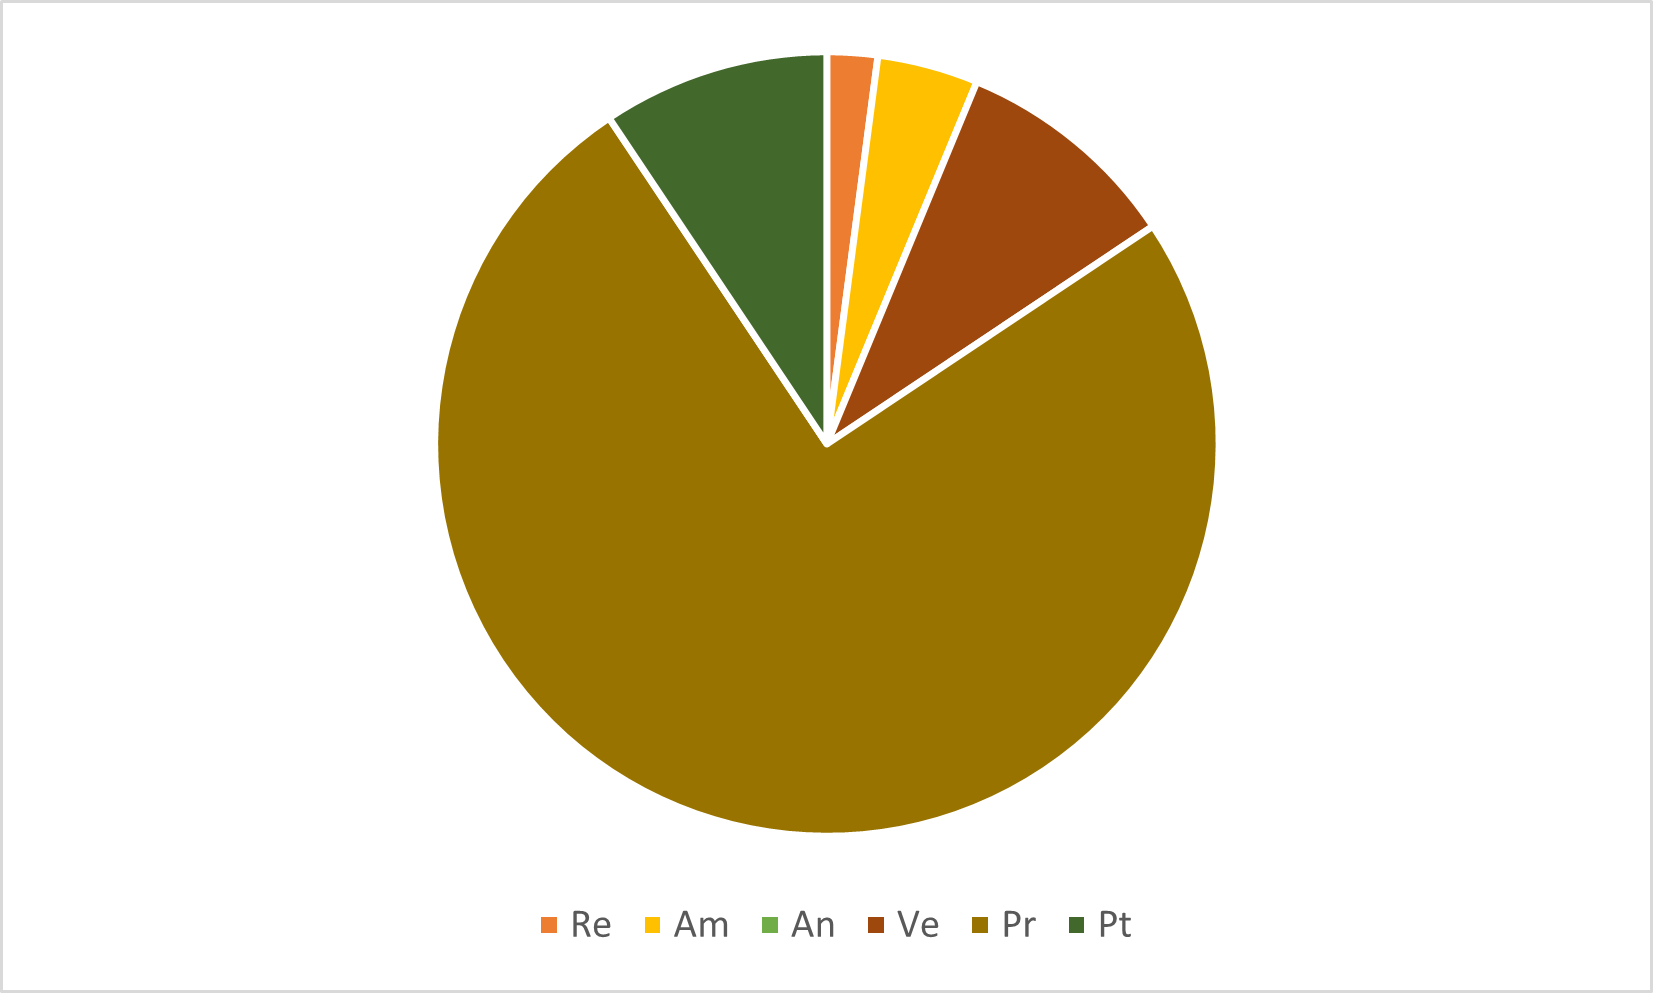
\includegraphics[scale=0.6]{img/grafi preventivo/torta/codifica/periodo2.png}
    \caption{Grafico a torta della ripartizione delle ore per ruolo nel secondo periodo della fase di progettazione di dettaglio e codifica}
\end{figure}
\subsubsubsection{Preventivo dei costi}
La seguente tabella rappresenta le ore dedicate ad ogni ruolo e il corrispettivo costo in euro per il secondo periodo della fase di progettazione di dettaglio e codifica:

	\setlength\extrarowheight{5pt}
	\rowcolors{2}{gray!10}{gray!40}
	\begin{tabularx}{\textwidth}{|ccc|c|}
		\hline
		\rowcolor{white}
		\textbf{Ruolo} & \textbf{Costo orario (€)} & \textbf{Ore totali} & \textbf{Costo totale (€)} \\
		\hline
		Responsabile &30&2&60 \\
		Amministratore &20&4&80 \\
		Analista &25&0&0 \\
		Verificatore &15&9&135 \\
		Programmatore &15&72&1080 \\
		Progettista &25&9&225 \\
		\hline
		Totale &-&-&1580 \\
		\hline
		\rowcolor{white}
		\caption{Prospetto del costo orario durante  il secondo periodo di progettazione di dettaglio e codifica per ruolo}
	\end{tabularx}
    \vspace{10pt}
	
%
% ----------------------------------------------------------------------------------------------------------------
\newpage
\subsubsection{Periodo 3}
% ----------------------------------------------------------------------------------------------------------------
%
\subsubsubsection{Preventivo orario}
La seguente tabella rappresenta la distribuzione oraria per ogni componente per il terzo periodo della fase di progettazione di dettaglio e codifica:

	\setlength\extrarowheight{5pt}
	\rowcolors{2}{gray!10}{gray!40}
	\begin{tabularx}{\textwidth}{|ccccccc|c|}
		\hline
		\rowcolor{white}
		\textbf{Nome} & \textbf{Re} & \textbf{Am} & \textbf{An} & \textbf{Ve} & \textbf{Pr}& \textbf{Pt} & \textbf{Ore totali} \\
		\hline
		Nicola Sinicato &0&0&3&0&0&0&3 \\
		Gabriele Da Re &1&2&0&0&0&0&3 \\
		Luca Brugnera &0&0&0&0&0&3&3 \\
		Matteo Stocco &0&0&3&0&0&0&3 \\
		Ana Lazic &1&2&0&0&0&0&3 \\
		Zhen Wei Zheng &1&0&0&0&0&2&3 \\
		\hline
		Ore totali ruolo &3&4&6&0&0&5&18 \\
		\hline
		\rowcolor{white}
		\caption{Distribuzione oraria durante  il terzo periodo di progettazione di dettaglio e codifica per ruolo e persona}
	\end{tabularx}
	\vspace{10pt}
	
\begin{figure}[H]
    \centering
    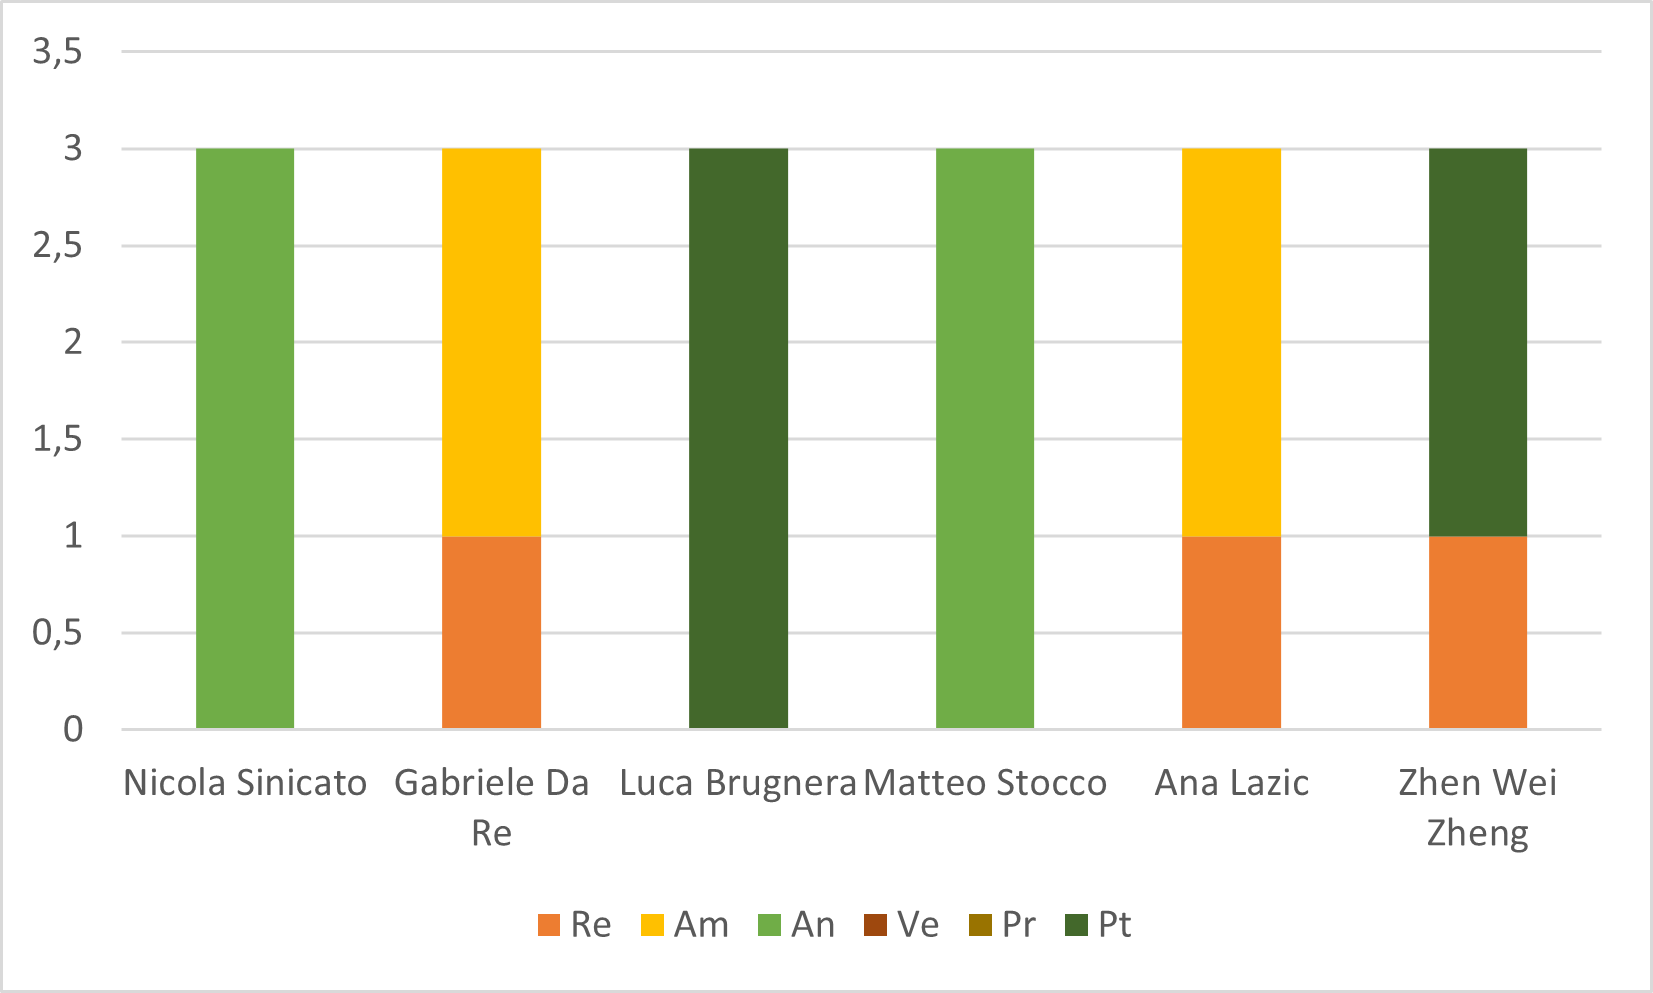
\includegraphics[scale=0.6]{img/grafi preventivo/istogrammi/codifica/periodo3.png}
    \caption{Istogramma della ripartizione delle ore del terzo periodo della fase di progettazione di dettaglio e codifica}
\end{figure}
\begin{figure}[H]
    \centering
    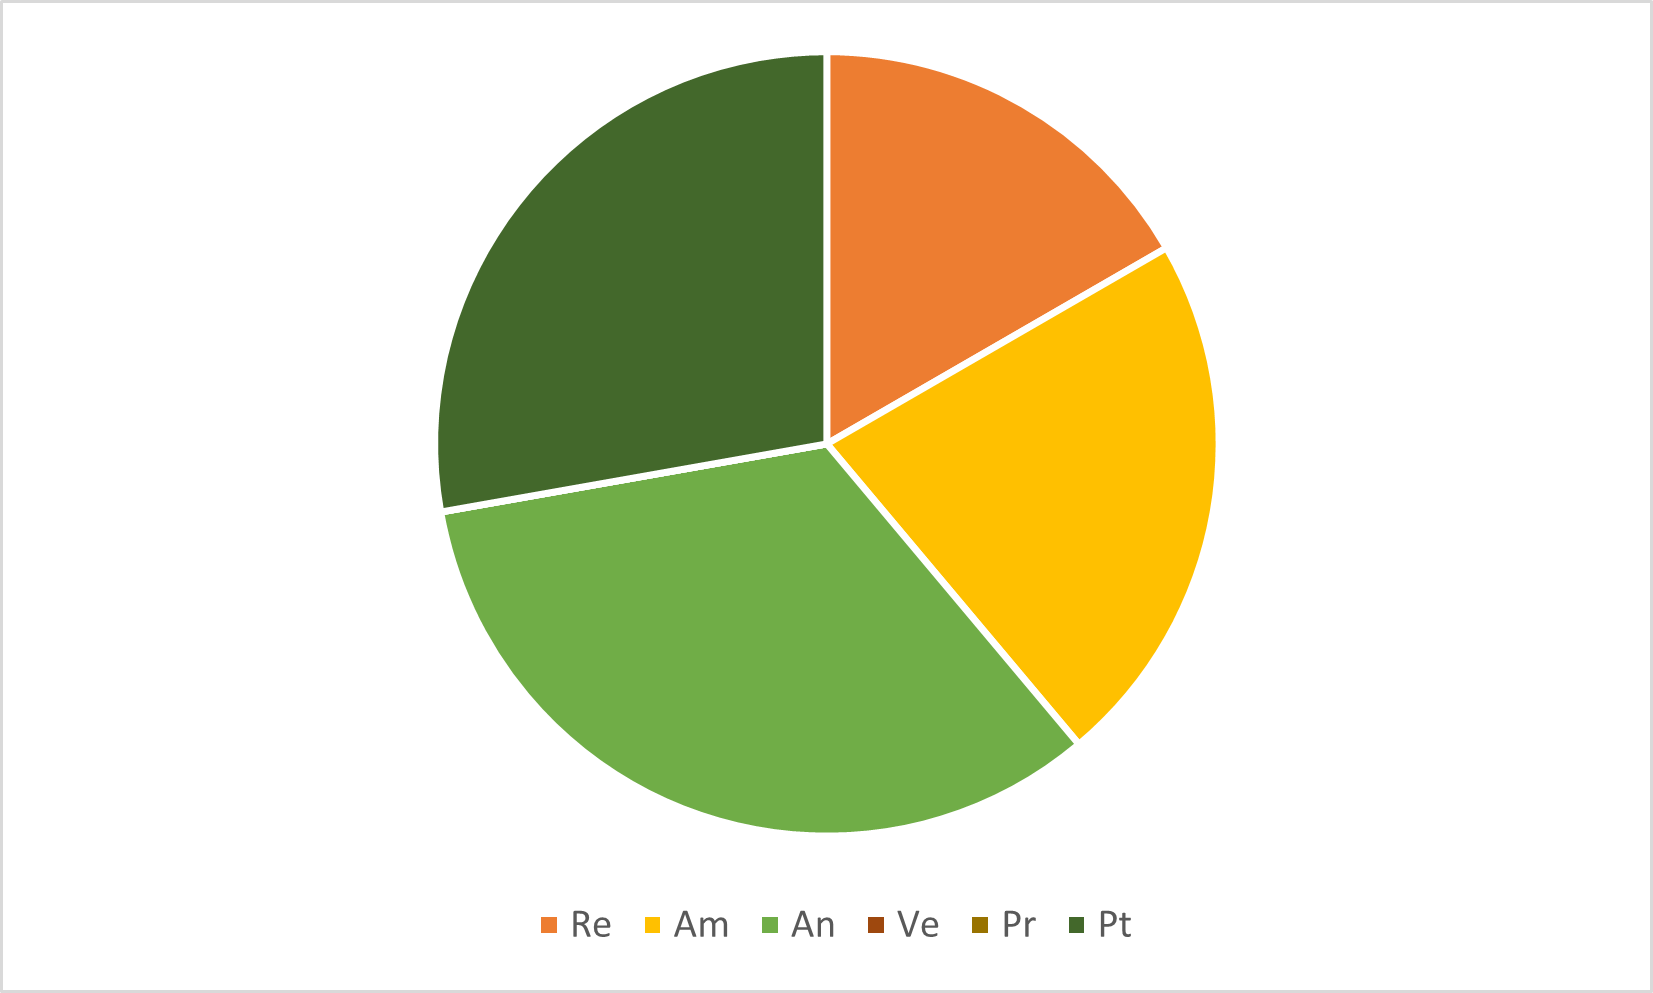
\includegraphics[scale=0.6]{img/grafi preventivo/torta/codifica/periodo3.png}
    \caption{Grafico a torta della ripartizione delle ore per ruolo nel terzo periodo della fase di progettazione di dettaglio e codifica}
\end{figure}
\subsubsubsection{Preventivo dei costi}
La seguente tabella rappresenta le ore dedicate ad ogni ruolo e il corrispettivo costo in euro per il terzo periodo della fase di progettazione di dettaglio e codifica:

	\setlength\extrarowheight{5pt}
	\rowcolors{2}{gray!10}{gray!40}
	\begin{tabularx}{\textwidth}{|ccc|c|}
		\hline
		\rowcolor{white}
		\textbf{Ruolo} & \textbf{Costo orario (€)} & \textbf{Ore totali} & \textbf{Costo totale (€)} \\
		\hline
		Responsabile &30&3&90 \\
		Amministratore &20&4&80 \\
		Analista &25&6&150 \\
		Verificatore &15&0&0 \\
		Programmatore &15&0&0 \\
		Progettista &25&5&125 \\
		\hline
		Totale &-&-&445 \\
		\hline
		\rowcolor{white}
		\caption{Prospetto del costo orario durante  il terzo periodo di progettazione di dettaglio e codifica per ruolo}
	\end{tabularx}
    \vspace{10pt}
	
%
% ----------------------------------------------------------------------------------------------------------------
\newpage
\subsubsection{Riepilogo della fase di progettazione di dettaglio e codifica}
% ----------------------------------------------------------------------------------------------------------------
%
\subsubsubsection{Preventivo orario}
La seguente tabella rappresenta la distribuzione oraria per ogni componente la fase di progettazione di dettaglio e codifica:

	\setlength\extrarowheight{5pt}
	\rowcolors{2}{gray!10}{gray!40}
	\begin{tabularx}{\textwidth}{|ccccccc|c|}
		\hline
		\rowcolor{white}
		\textbf{Nome} & \textbf{Re} & \textbf{Am} & \textbf{An} & \textbf{Ve} & \textbf{Pr}& \textbf{Pt} & \textbf{Ore totali} \\
		\hline
		Nicola Sinicato &1&0&5&2&14&0&22 \\
		Gabriele Da Re &1&3&0&1&11&6&22 \\
		Luca Brugnera &0&2&0&2&11&7&22 \\
		Matteo Stocco &1&0&3&2&14&2&22 \\
		Ana Lazic &2&2&3&2&11&2&22 \\
		Zhen Wei Zheng &2&3&0&4&11&2&22 \\
		\hline
		Ore totali ruolo &7&10&11&13&72&19&132 \\
		\hline
		\rowcolor{white}
		\caption{Distribuzione oraria durante la fase di progettazione di dettaglio e codifica per ruolo e persona}
	\end{tabularx}
	\vspace{10pt}
	
\begin{figure}[H]
    \centering
    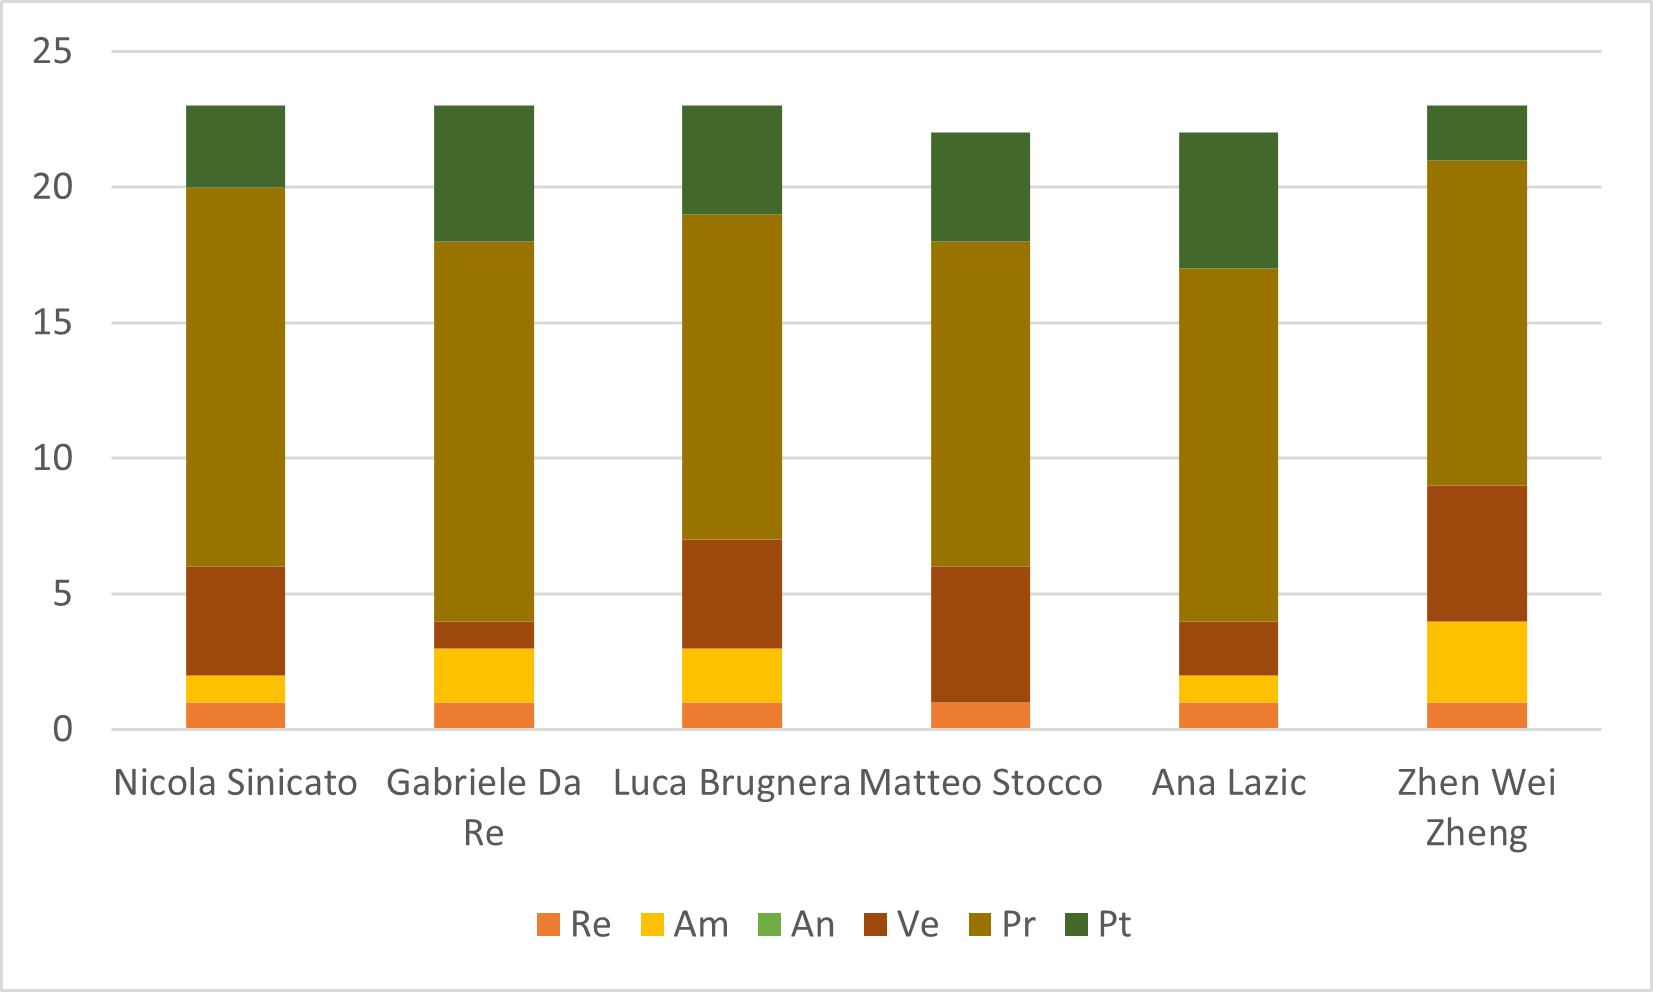
\includegraphics[scale=0.6]{img/grafi preventivo/istogrammi/codifica/complessivo.png}
    \caption{Istogramma della ripartizione delle ore della fase di progettazione di dettaglio e codifica}
\end{figure}
\begin{figure}[H]
    \centering
    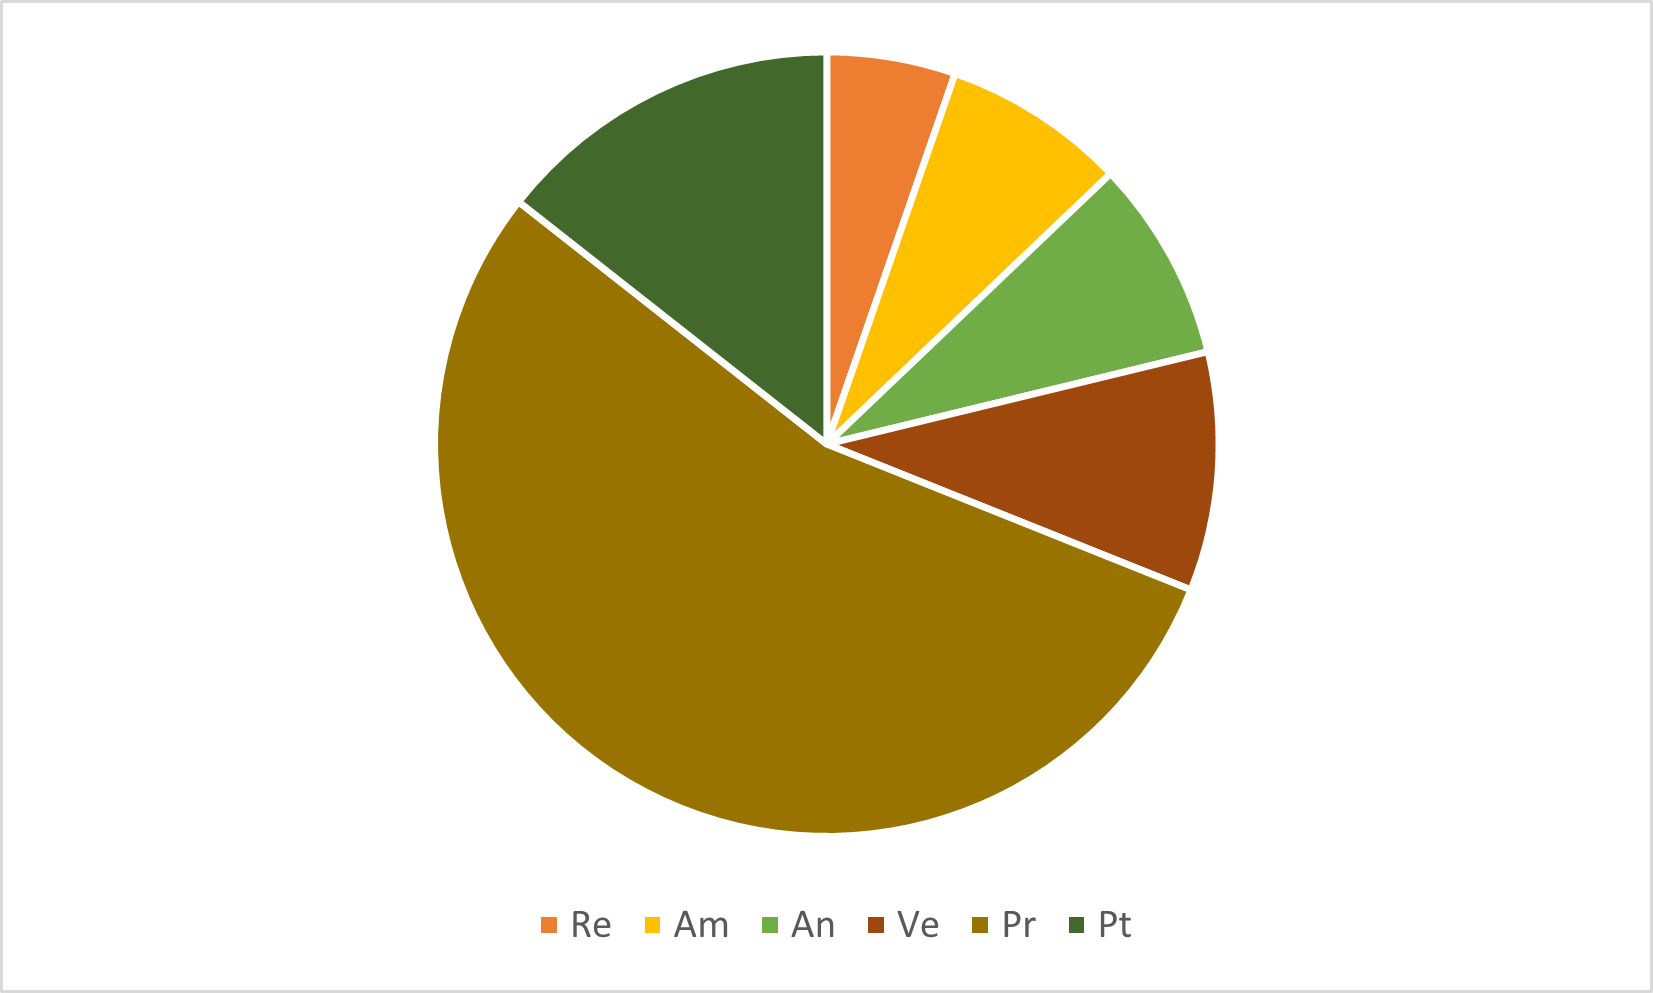
\includegraphics[scale=0.6]{img/grafi preventivo/torta/codifica/complessivo.png}
    \caption{Grafico a torta della ripartizione delle ore per ruolo nella fase di progettazione di dettaglio e codifica}
\end{figure}
\subsubsubsection{Preventivo dei costi}
La seguente tabella rappresenta le ore dedicate ad ogni ruolo e il corrispettivo costo in euro per la fase di progettazione di dettaglio e codifica:

	\setlength\extrarowheight{5pt}
	\rowcolors{2}{gray!10}{gray!40}
	\begin{tabularx}{\textwidth}{|ccc|c|}
		\hline
		\rowcolor{white}
		\textbf{Ruolo} & \textbf{Costo orario (€)} & \textbf{Ore totali} & \textbf{Costo totale (€)} \\
		\hline
		Responsabile &30&7&210 \\
		Amministratore &20&10&200 \\
		Analista &25&11&275 \\
		Verificatore &15&13&195 \\
		Programmatore &15&72&1080 \\
		Progettista &25&19&475 \\
		\hline
		Totale &-&-&2435 \\
		\hline
		\rowcolor{white}
		\caption{Prospetto del costo orario durante la fase di progettazione di dettaglio e codifica per ruolo}
	\end{tabularx}
    \vspace{10pt}
	
% ----------------------------------------------------------------------------------------------------------------
\newpage
\subsection{Validazione e collaudo}

% ----------------------------------------------------------------------------------------------------------------
\subsubsection{Periodo 1}
% ----------------------------------------------------------------------------------------------------------------
%
\subsubsubsection{Preventivo orario}
La seguente tabella rappresenta la distribuzione oraria per ogni componente per il primo periodo della fase di validazione e collaudo:

	\setlength\extrarowheight{5pt}
	\rowcolors{2}{gray!10}{gray!40}
	\begin{tabularx}{\textwidth}{|ccccccc|c|}
		\hline
		\rowcolor{white}
		\textbf{Nome} & \textbf{Re} & \textbf{Am} & \textbf{An} & \textbf{Ve} & \textbf{Pr}& \textbf{Pt} & \textbf{Ore totali} \\
		\hline
		Nicola Sinicato &0&0&0&2&3&6&11 \\
		Gabriele Da Re &2&1&0&0&5&3&11 \\
		Luca Brugnera &1&2&0&0&4&4&11 \\
		Matteo Stocco &1&3&0&4&3&0&11 \\
		Ana Lazic &1&0&0&3&4&3&11 \\
		Zhen Wei Zheng &4&3&0&4&0&0&11 \\
		\hline
		Ore totali ruolo &9&9&0&13&19&16&66 \\
		\hline
		\rowcolor{white}
		\caption{Distribuzione oraria durante  il primo periodo di validazione e collaudo per ruolo e persona}
	\end{tabularx}
	\vspace{10pt}
	
\begin{figure}[H]
    \centering
    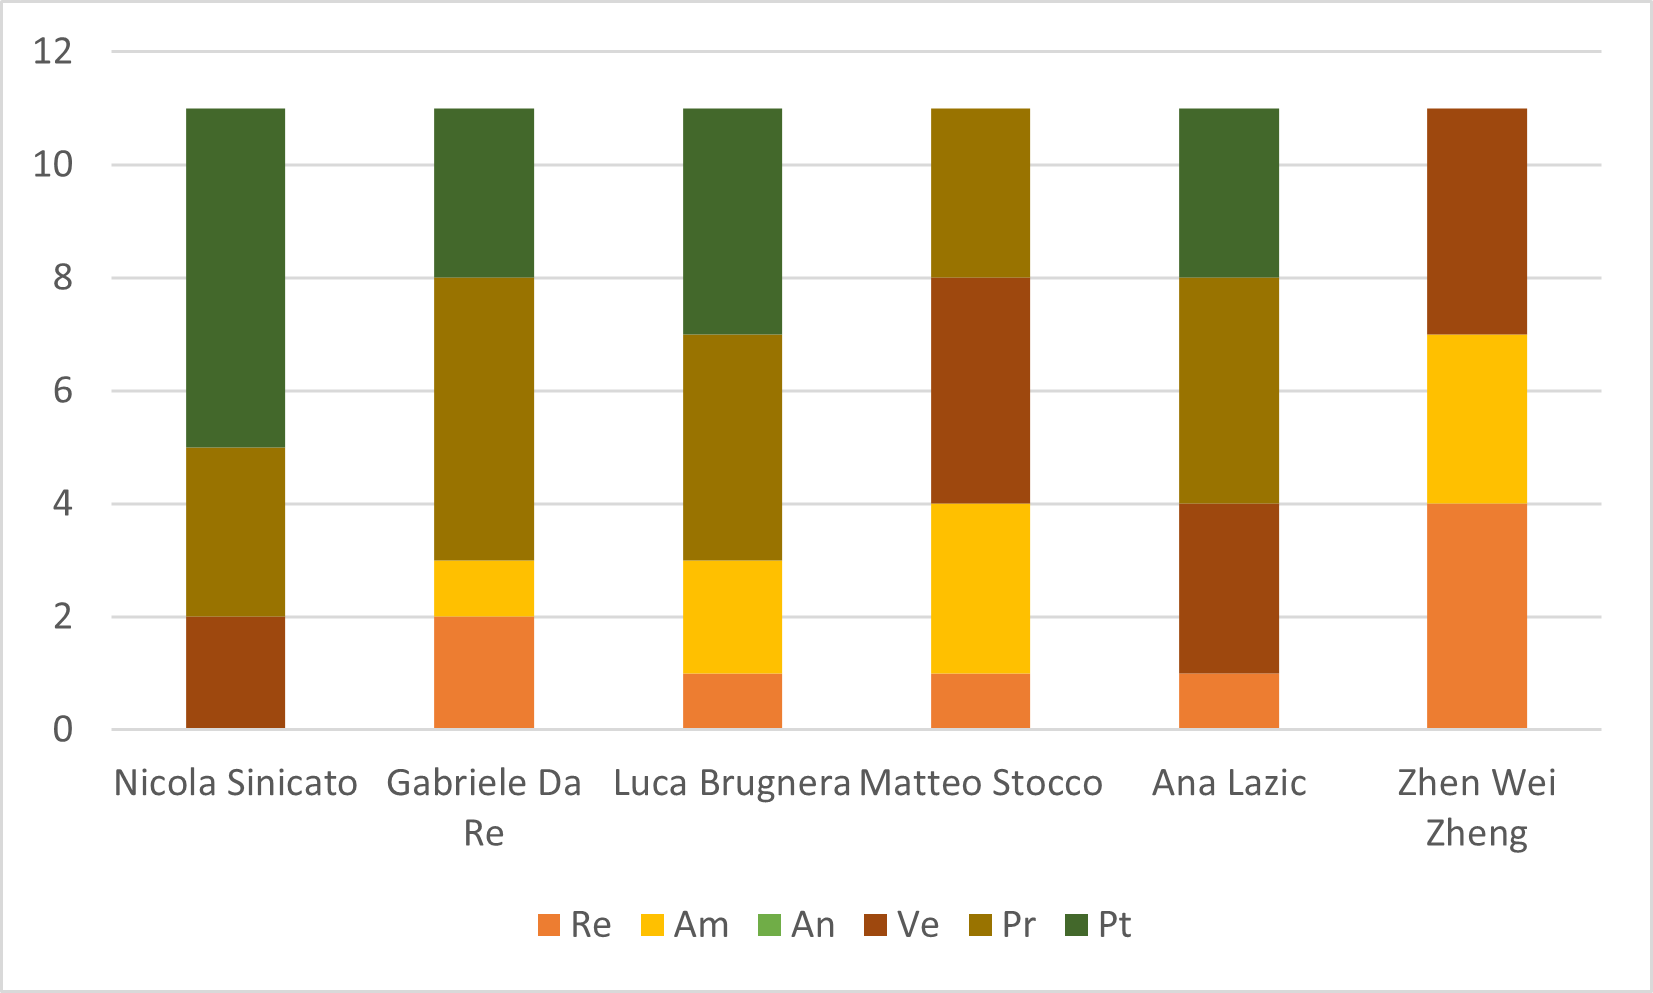
\includegraphics[scale=0.6]{img/grafi preventivo/istogrammi/validazione/periodo1.png}
    \caption{Istogramma della ripartizione delle ore del primo periodo della fase di validazione e collaudo}
\end{figure}
\begin{figure}[H]
    \centering
    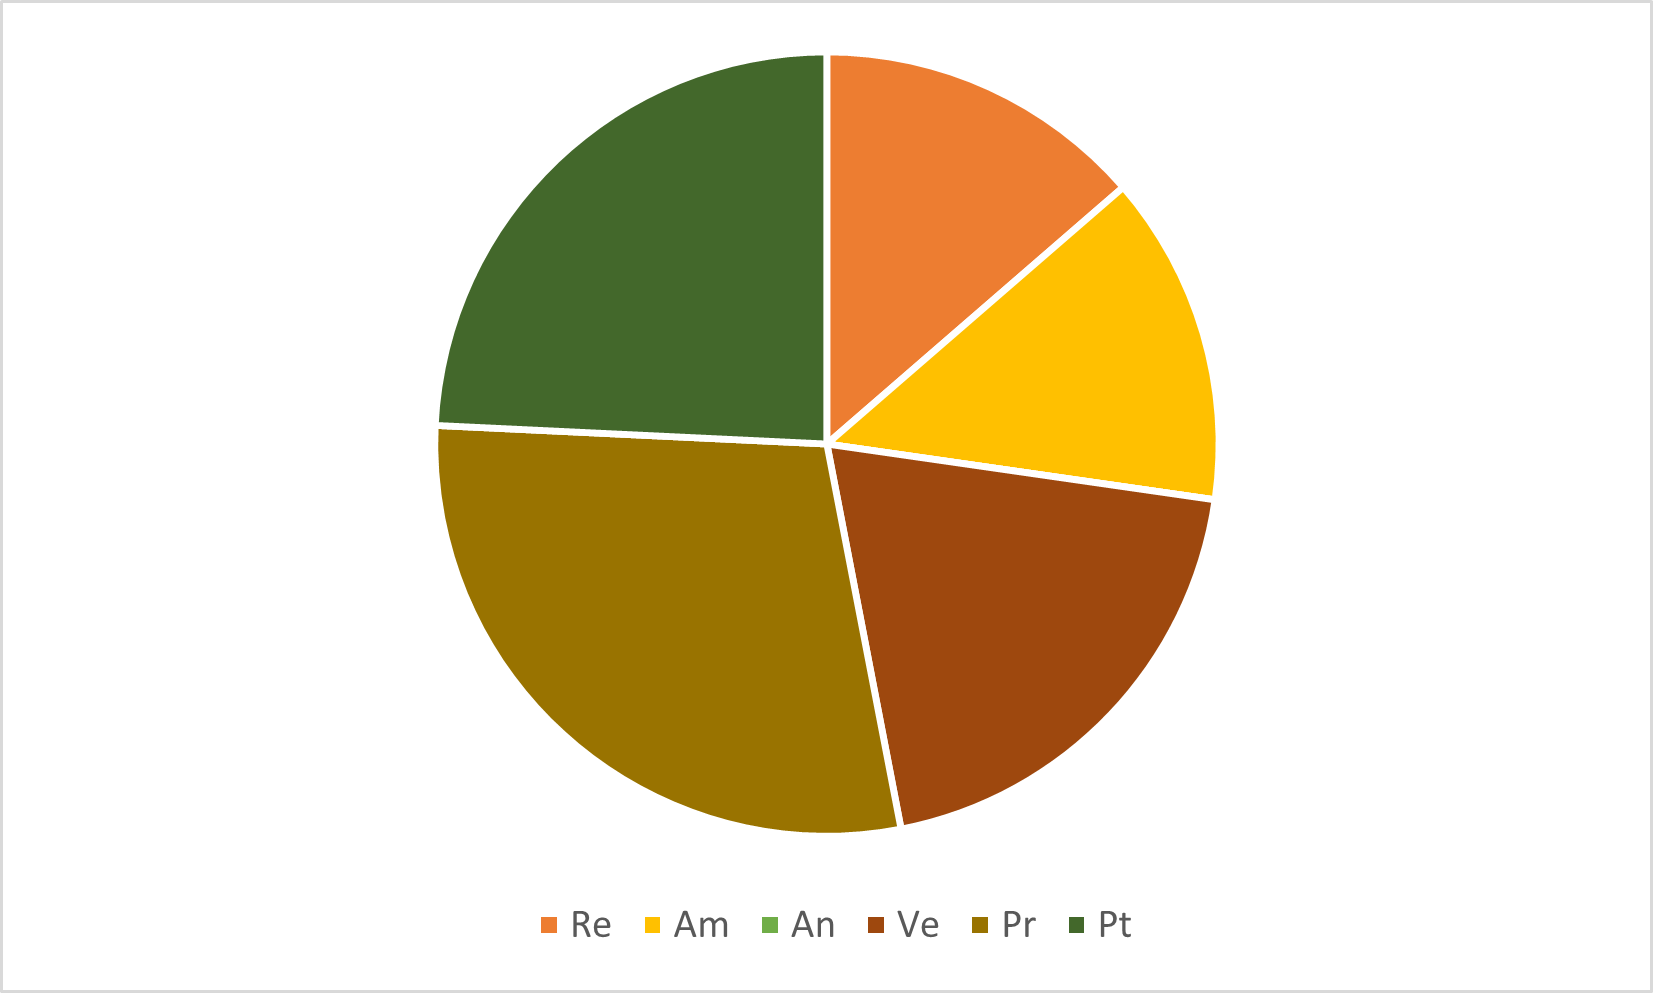
\includegraphics[scale=0.6]{img/grafi preventivo/torta/validazione/periodo1.png}
    \caption{Grafico a torta della ripartizione delle ore per ruolo nel primo periodo della fase di validazione e collaudo}
\end{figure}
\subsubsubsection{Preventivo dei costi}
La seguente tabella rappresenta le ore dedicate ad ogni ruolo e il corrispettivo costo in euro per il primo periodo della fase di validazione e collaudo:

	\setlength\extrarowheight{5pt}
	\rowcolors{2}{gray!10}{gray!40}
	\begin{tabularx}{\textwidth}{|ccc|c|}
		\hline
		\rowcolor{white}
		\textbf{Ruolo} & \textbf{Costo orario (€)} & \textbf{Ore totali} & \textbf{Costo totale (€)} \\
		\hline
		Responsabile &30&9&270 \\
		Amministratore &20&9&180 \\
		Analista &25&0&0 \\
		Verificatore &15&13&195 \\
		Programmatore &15&19&285 \\
		Progettista &25&16&400 \\
		\hline
		Totale &-&-&1330 \\
		\hline
		\rowcolor{white}
		\caption{Prospetto del costo orario durante il primo periodo di validazione e collaudo per ruolo}
	\end{tabularx}
    \vspace{10pt}
	
% ----------------------------------------------------------------------------------------------------------------
\newpage
\subsubsection{Periodo 2}
% ----------------------------------------------------------------------------------------------------------------
%
\subsubsubsection{Preventivo orario}
La seguente tabella rappresenta la distribuzione oraria per ogni componente per il secondo periodo della fase di validazione e collaudo:

	\setlength\extrarowheight{5pt}
	\rowcolors{2}{gray!10}{gray!40}
	\begin{tabularx}{\textwidth}{|ccccccc|c|}
		\hline
		\rowcolor{white}
		\textbf{Nome} & \textbf{Re} & \textbf{Am} & \textbf{An} & \textbf{Ve} & \textbf{Pr}& \textbf{Pt} & \textbf{Ore totali} \\
		\hline
		Nicola Sinicato &2&0&0&2&0&0&4 \\
		Gabriele Da Re &1&3&0&0&0&0&4 \\
		Luca Brugnera &0&0&0&2&2&0&4 \\
		Matteo Stocco &2&0&0&0&2&0&4 \\
		Ana Lazic &0&0&3&1&0&0&4 \\
		Zhen Wei Zheng &1&0&0&3&0&0&4 \\
		\hline
		Ore totali ruolo &6&3&3&8&4&0&24 \\
		\hline
		\rowcolor{white}
		\caption{Distribuzione oraria durante  il secondo periodo di validazione e collaudo per ruolo e persona}
	\end{tabularx}
	\vspace{10pt}
	

\begin{figure}[H]
    \centering
    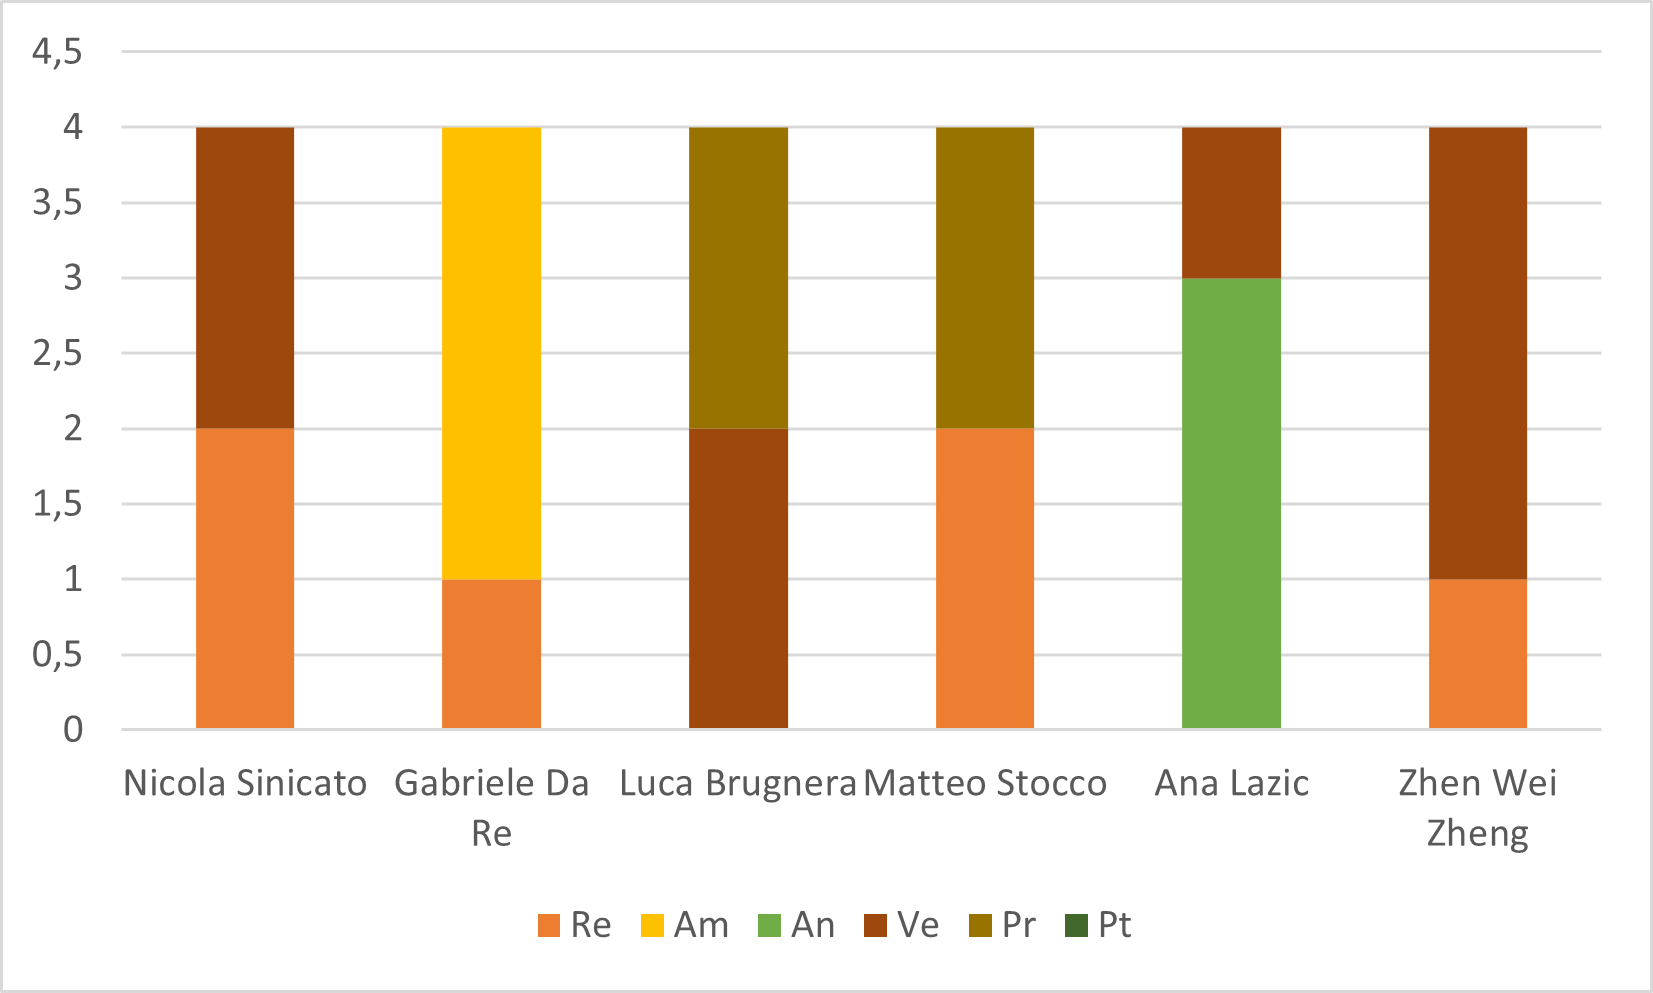
\includegraphics[scale=0.6]{img/grafi preventivo/istogrammi/validazione/periodo2.png}
    \caption{Istogramma della ripartizione delle ore del secondo periodo della fase di validazione e collaudo}
\end{figure}
\begin{figure}[H]
    \centering
    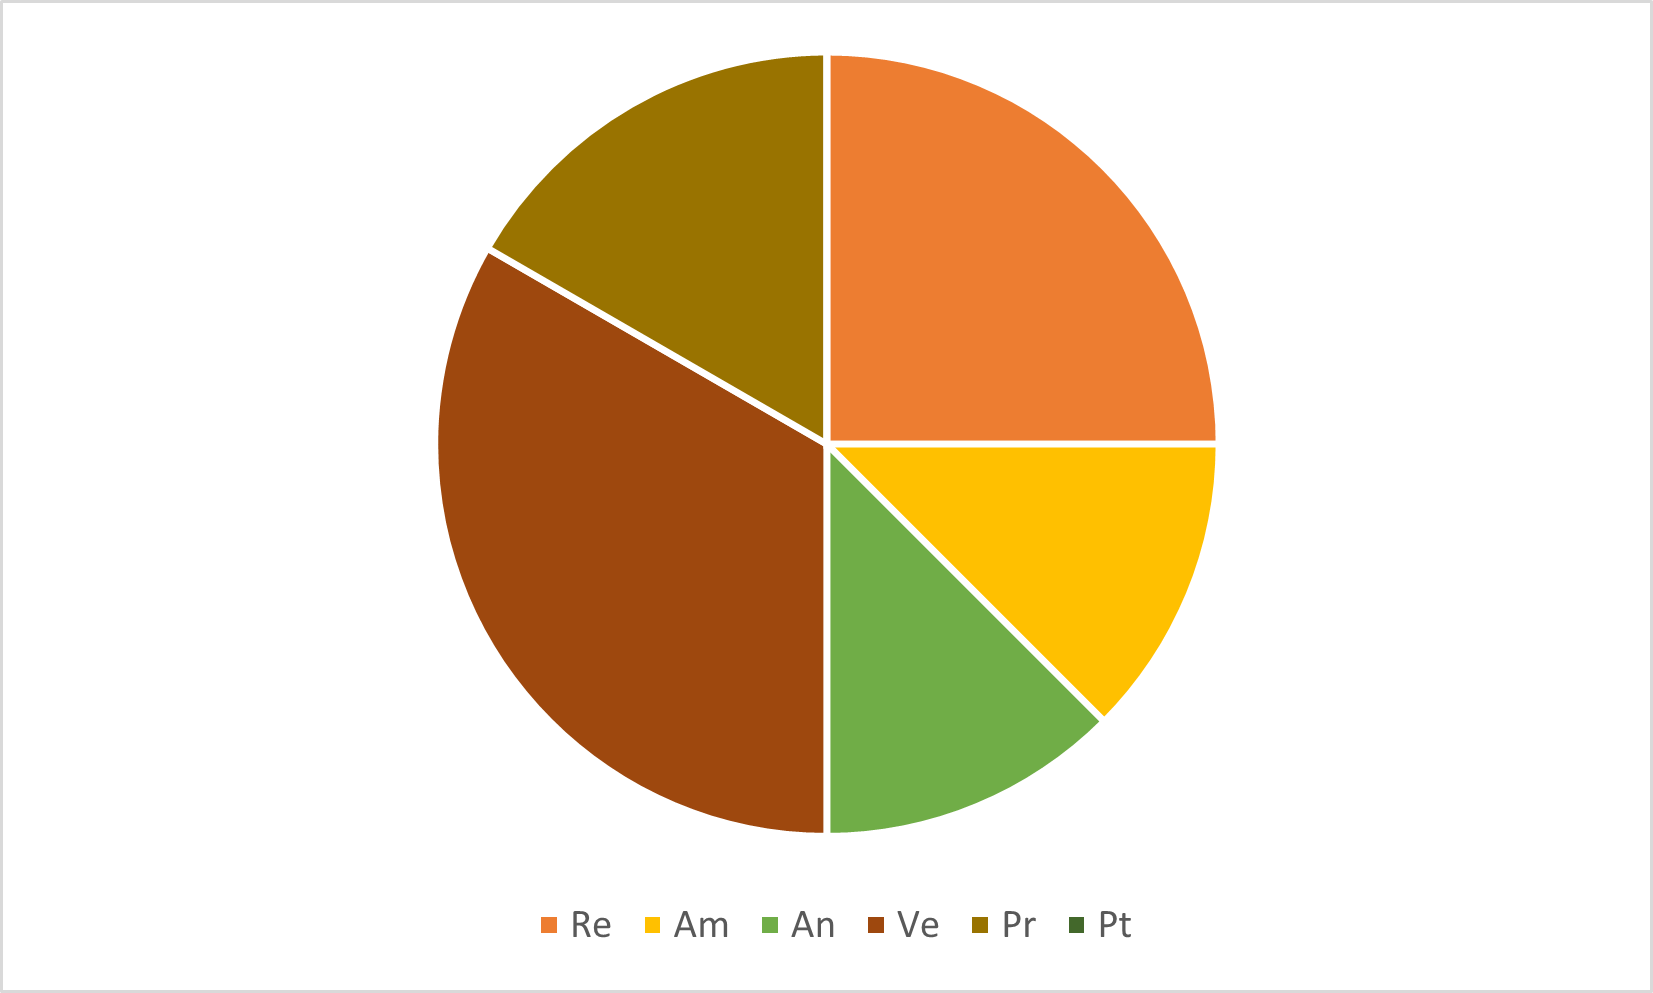
\includegraphics[scale=0.6]{img/grafi preventivo/torta/validazione/periodo2.png}
    \caption{Grafico a torta della ripartizione delle ore per ruolo nel secondo periodo della fase di validazione e collaudo}
\end{figure}
\subsubsubsection{Preventivo dei costi}
La seguente tabella rappresenta le ore dedicate ad ogni ruolo e il corrispettivo costo in euro per il secondo periodo della fase di validazione e collaudo:

	\setlength\extrarowheight{5pt}
	\rowcolors{2}{gray!10}{gray!40}
	\begin{tabularx}{\textwidth}{|ccc|c|}
		\hline
		\rowcolor{white}
		\textbf{Ruolo} & \textbf{Costo orario (€)} & \textbf{Ore totali} & \textbf{Costo totale (€)} \\
		\hline
		Responsabile &30&6&180 \\
		Amministratore &20&3&60 \\
		Analista &25&3&75 \\
		Verificatore &15&8&120 \\
		Programmatore &15&4&60 \\
		Progettista &25&0&0 \\
		\hline
		Totale &-&-&495 \\
		\hline
		\rowcolor{white}
		\caption{Prospetto del costo orario durante  il secondo periodo di validazione e collaudo per ruolo}
	\end{tabularx}
    \vspace{10pt}
	
% ----------------------------------------------------------------------------------------------------------------
\newpage
\subsubsection{Riepilogo della fase di validazione e collaudo }
% ----------------------------------------------------------------------------------------------------------------
%
\subsubsubsection{Preventivo orario}
La seguente tabella rappresenta la distribuzione oraria per ogni componente per la fase di validazione e collaudo:

	\setlength\extrarowheight{5pt}
	\rowcolors{2}{gray!10}{gray!40}
	\begin{tabularx}{\textwidth}{|ccccccc|c|}
		\hline
		\rowcolor{white}
		\textbf{Nome} & \textbf{Re} & \textbf{Am} & \textbf{An} & \textbf{Ve} & \textbf{Pr}& \textbf{Pt} & \textbf{Ore totali} \\
		\hline
		Nicola Sinicato &2&0&0&4&3&6&15 \\
		Gabriele Da Re &3&4&0&0&5&3&15 \\
		Luca Brugnera &1&2&0&2&6&4&15 \\
		Matteo Stocco &3&3&0&4&5&0&15 \\
		Ana Lazic &1&0&3&4&4&3&15 \\
		Zhen Wei Zheng &5&3&0&7&0&0&15 \\
		\hline
		Ore totali ruolo &15&12&3&21&23&16&90 \\
		\hline
		\rowcolor{white}
		\caption{Distribuzione oraria durante la fase di validazione e collaudo per ruolo e persona}
	\end{tabularx}
	\vspace{10pt}
	
\begin{figure}[H]
    \centering
    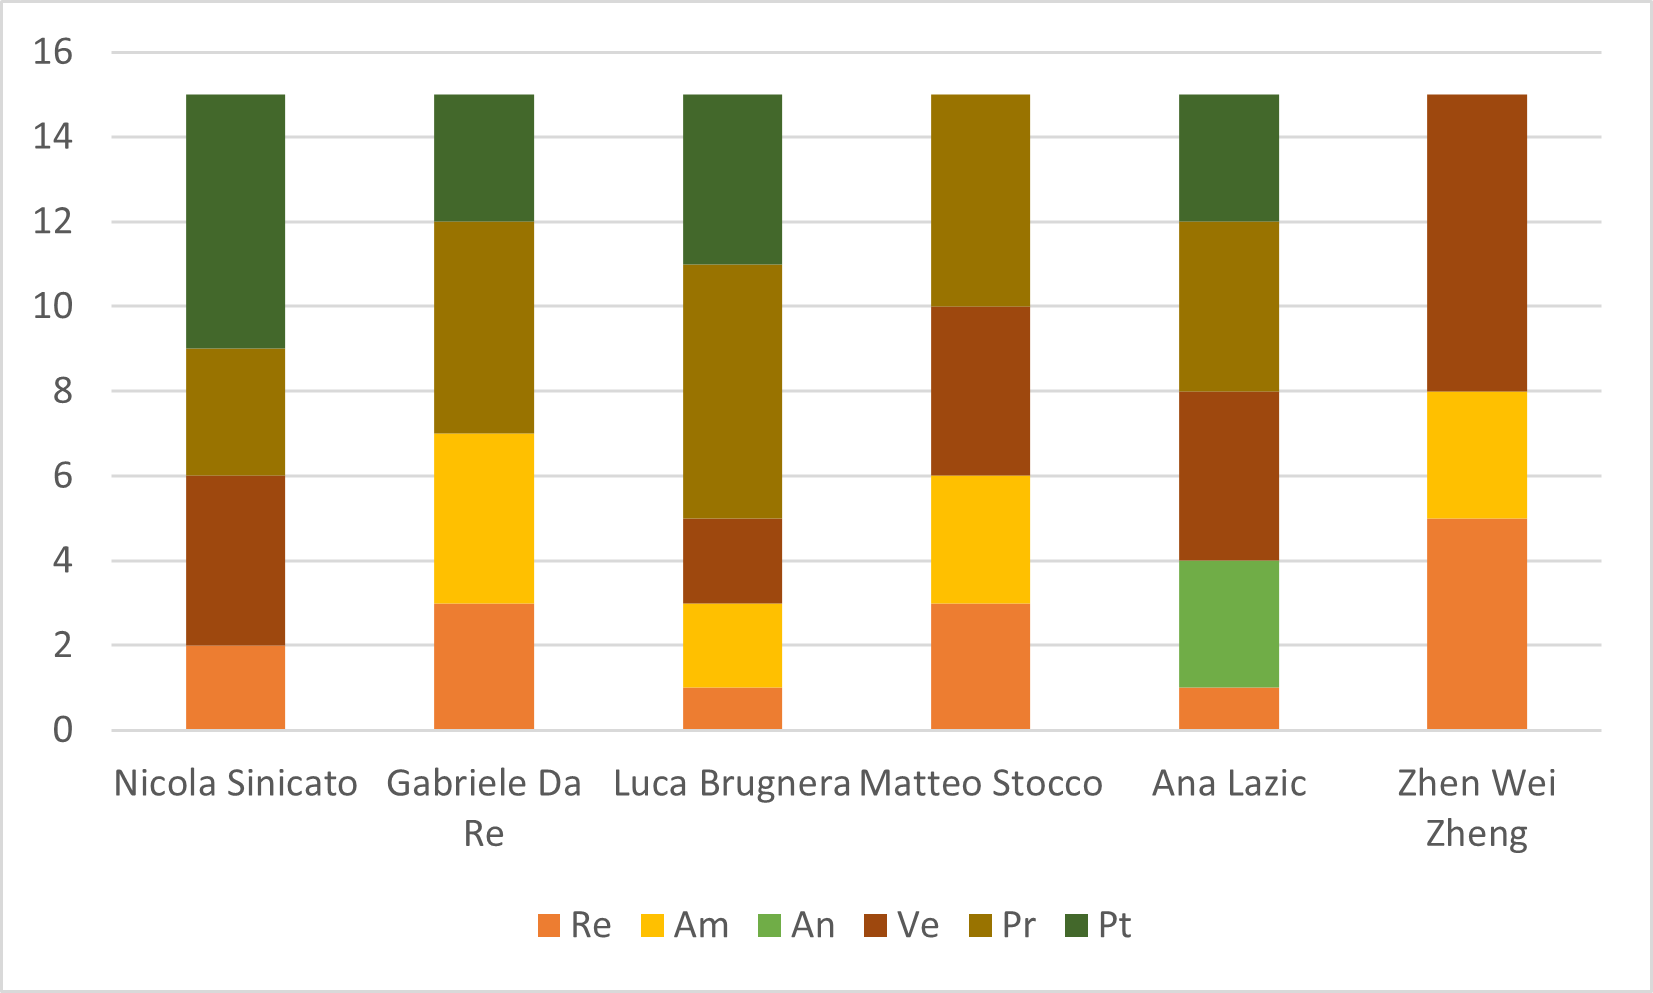
\includegraphics[scale=0.6]{img/grafi preventivo/istogrammi/validazione/complessivo.png}
    \caption{Istogramma della ripartizione delle ore della fase di validazione e collaudo}
\end{figure}
\begin{figure}[H]
    \centering
    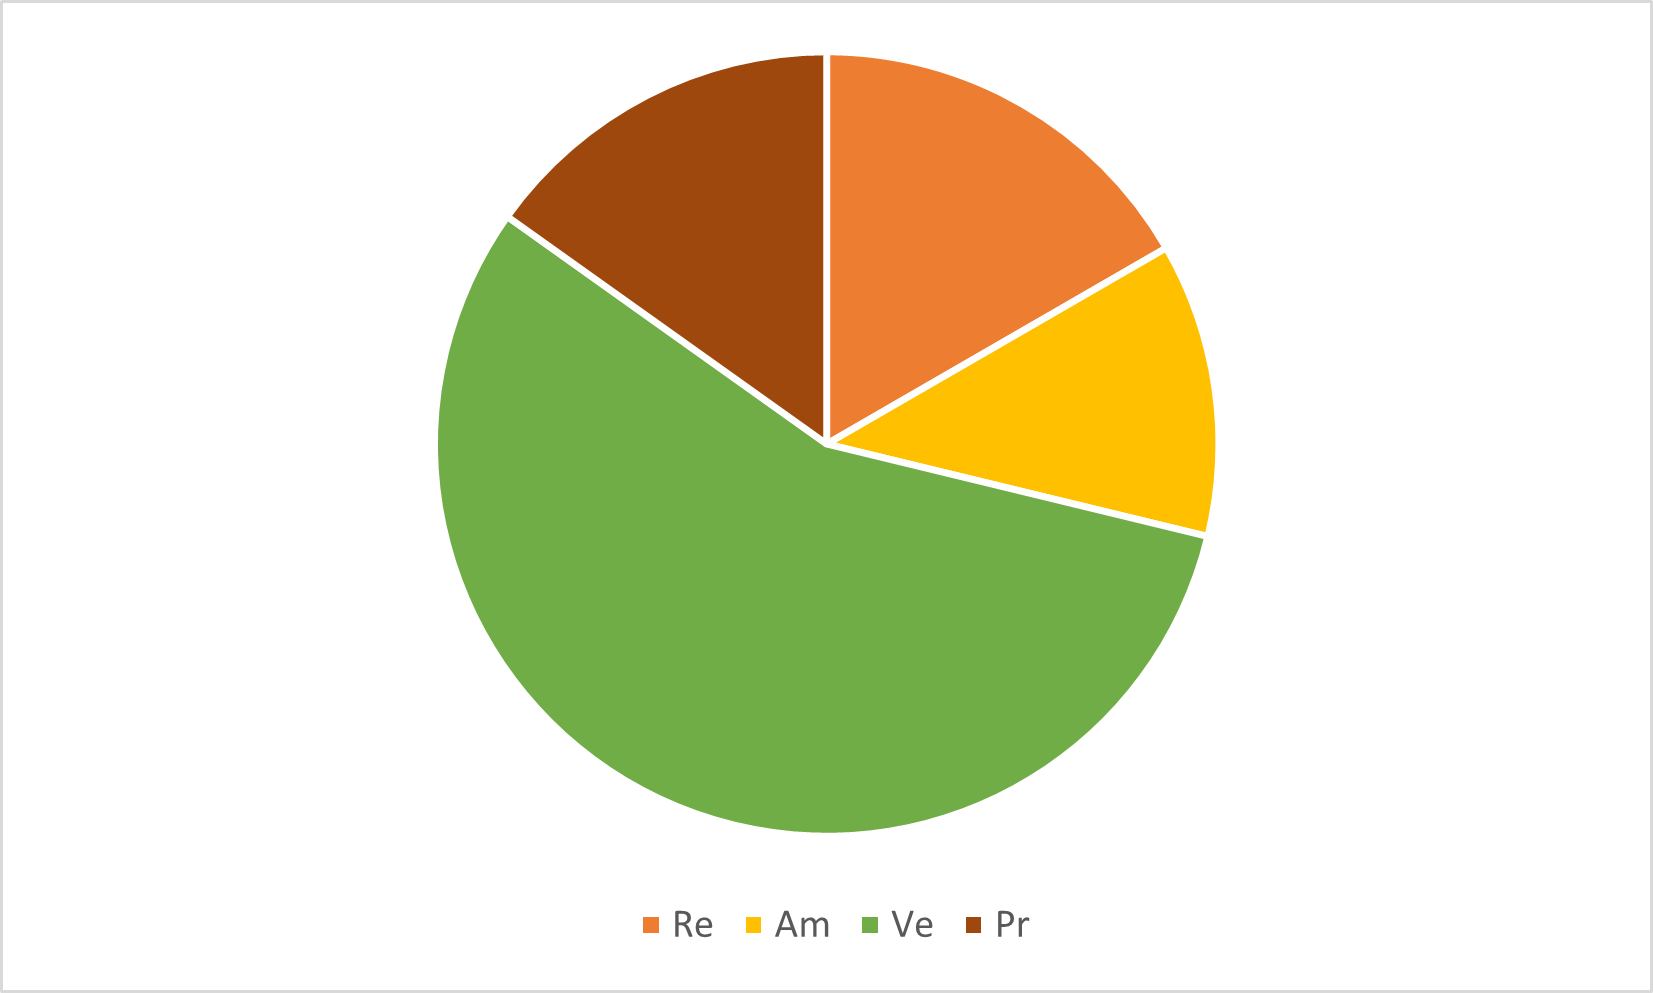
\includegraphics[scale=0.6]{img/grafi preventivo/torta/validazione/complessivo.png}
    \caption{Grafico a torta della ripartizione delle ore per ruolo nella fase di validazione e collaudo}
\end{figure}
\subsubsubsection{Preventivo dei costi}
La seguente tabella rappresenta le ore dedicate ad ogni ruolo e il corrispettivo costo in euro per la fase di validazione e collaudo:

	\setlength\extrarowheight{5pt}
	\rowcolors{2}{gray!10}{gray!40}
	\begin{tabularx}{\textwidth}{|ccc|c|}
		\hline
		\rowcolor{white}
		\textbf{Ruolo} & \textbf{Costo orario (€)} & \textbf{Ore totali} & \textbf{Costo totale (€)} \\
		\hline
		Responsabile &30&15&450 \\
		Amministratore &20&12&240 \\
		Analista &25&3&75 \\
		Verificatore &15&21&315 \\
		Programmatore &15&23&345 \\
		Progettista &25&16&400 \\
		\hline
		Totale &-&-&1825 \\
		\hline
		\rowcolor{white}
		\caption{Prospetto del costo orario durante la fase di validazione e collaudo per ruolo}
	\end{tabularx}
    \vspace{10pt}
	
%

% ----------------------------------------------------------------------------------------------------------------
\newpage
\subsection{Riepilogo complessivo}
% ----------------------------------------------------------------------------------------------------------------
%
\subsubsection{Preventivo orario}
La seguente tabella rappresenta la distribuzione oraria totale per ogni componente:

	\setlength\extrarowheight{5pt}
	\rowcolors{2}{gray!10}{gray!40}
	\begin{tabularx}{\textwidth}{|ccccccc|c|}
		\hline
		\rowcolor{white}
		\textbf{Nome} & \textbf{Re} & \textbf{Am} & \textbf{An} & \textbf{Ve} & \textbf{Pr}& \textbf{Pt} & \textbf{Ore totali} \\
		\hline
		Nicola Sinicato &10&8&21&13&22&16&90 \\
		Gabriele Da Re &9&21&13&9&17&21&90 \\
		Luca Brugnera &4&18&17&11&20&20&90 \\
		Matteo Stocco &9&12&17&20&21&11&90 \\
		Ana Lazic &7&8&27&13&19&16&90 \\
		Zhen Wei Zheng &11&13&15&24&11&16&90 \\
		\hline
		Ore totali ruolo &50&80&110&90&110&100&540 \\
		\hline
		\rowcolor{white}
		\caption{Ripartizione globale delle ore per ruolo e persona}
	\end{tabularx}
	\vspace{10pt}
	
\begin{figure}[H]
    \centering
    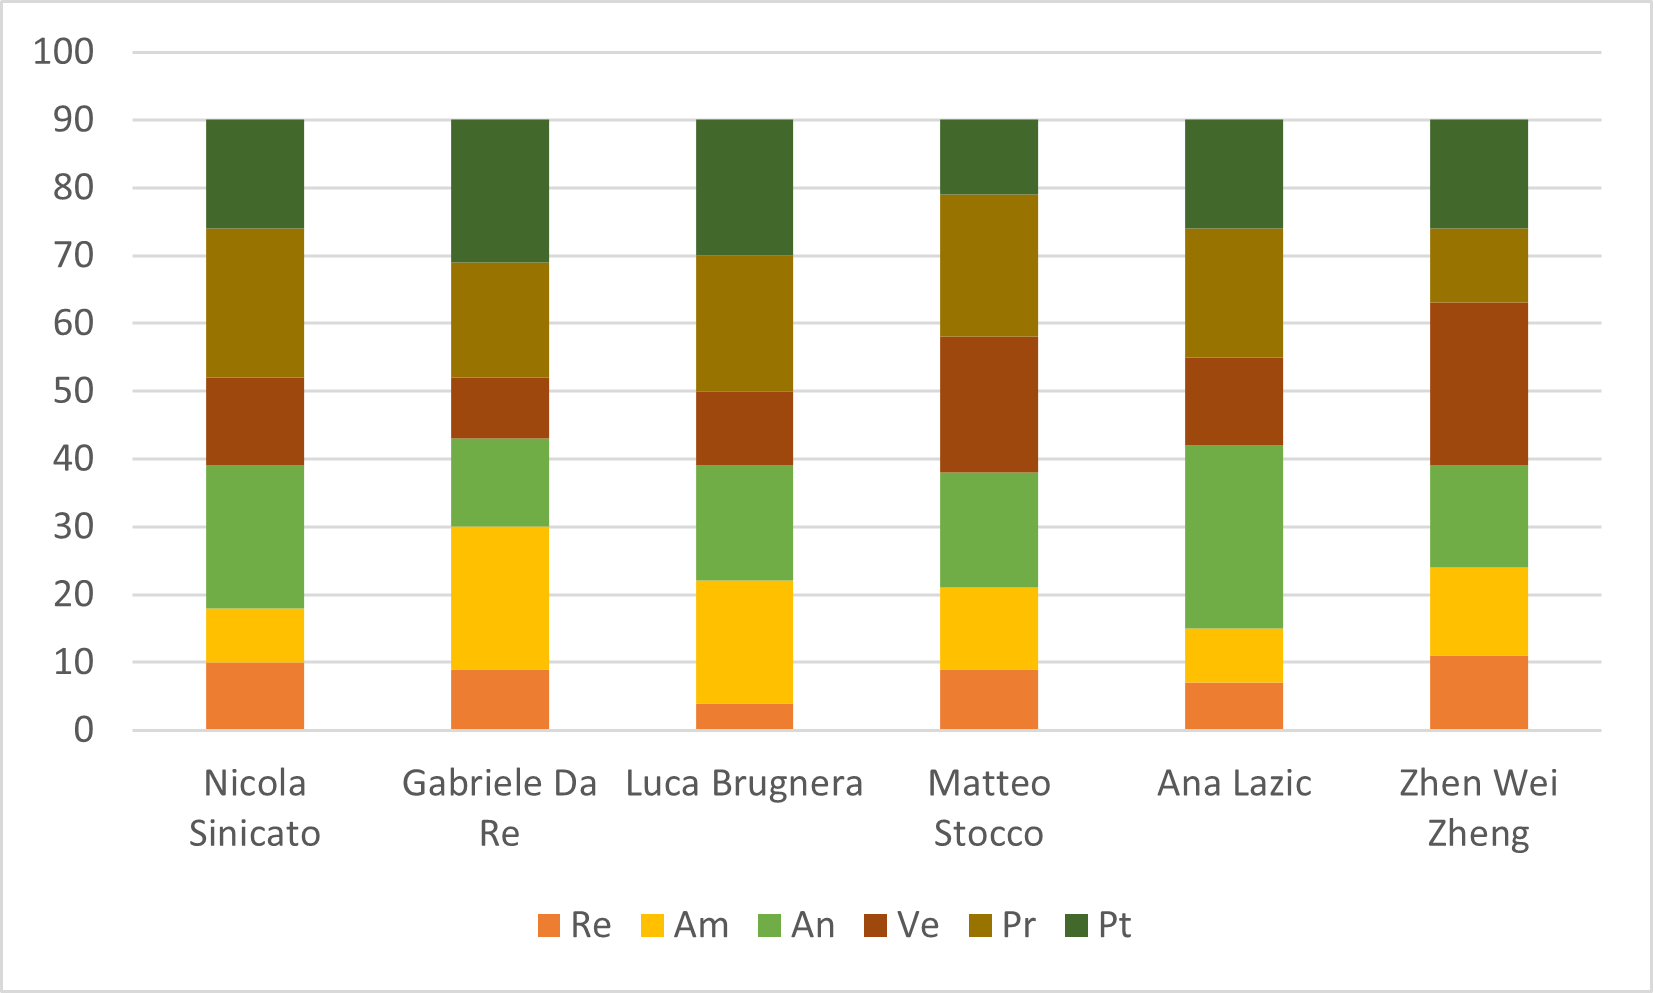
\includegraphics[scale=0.6]{img/grafi preventivo/istogrammi/totale/totale.png}
    \caption{Istogramma della distribuzione oraria}
\end{figure}
\begin{figure}[H]
    \centering
    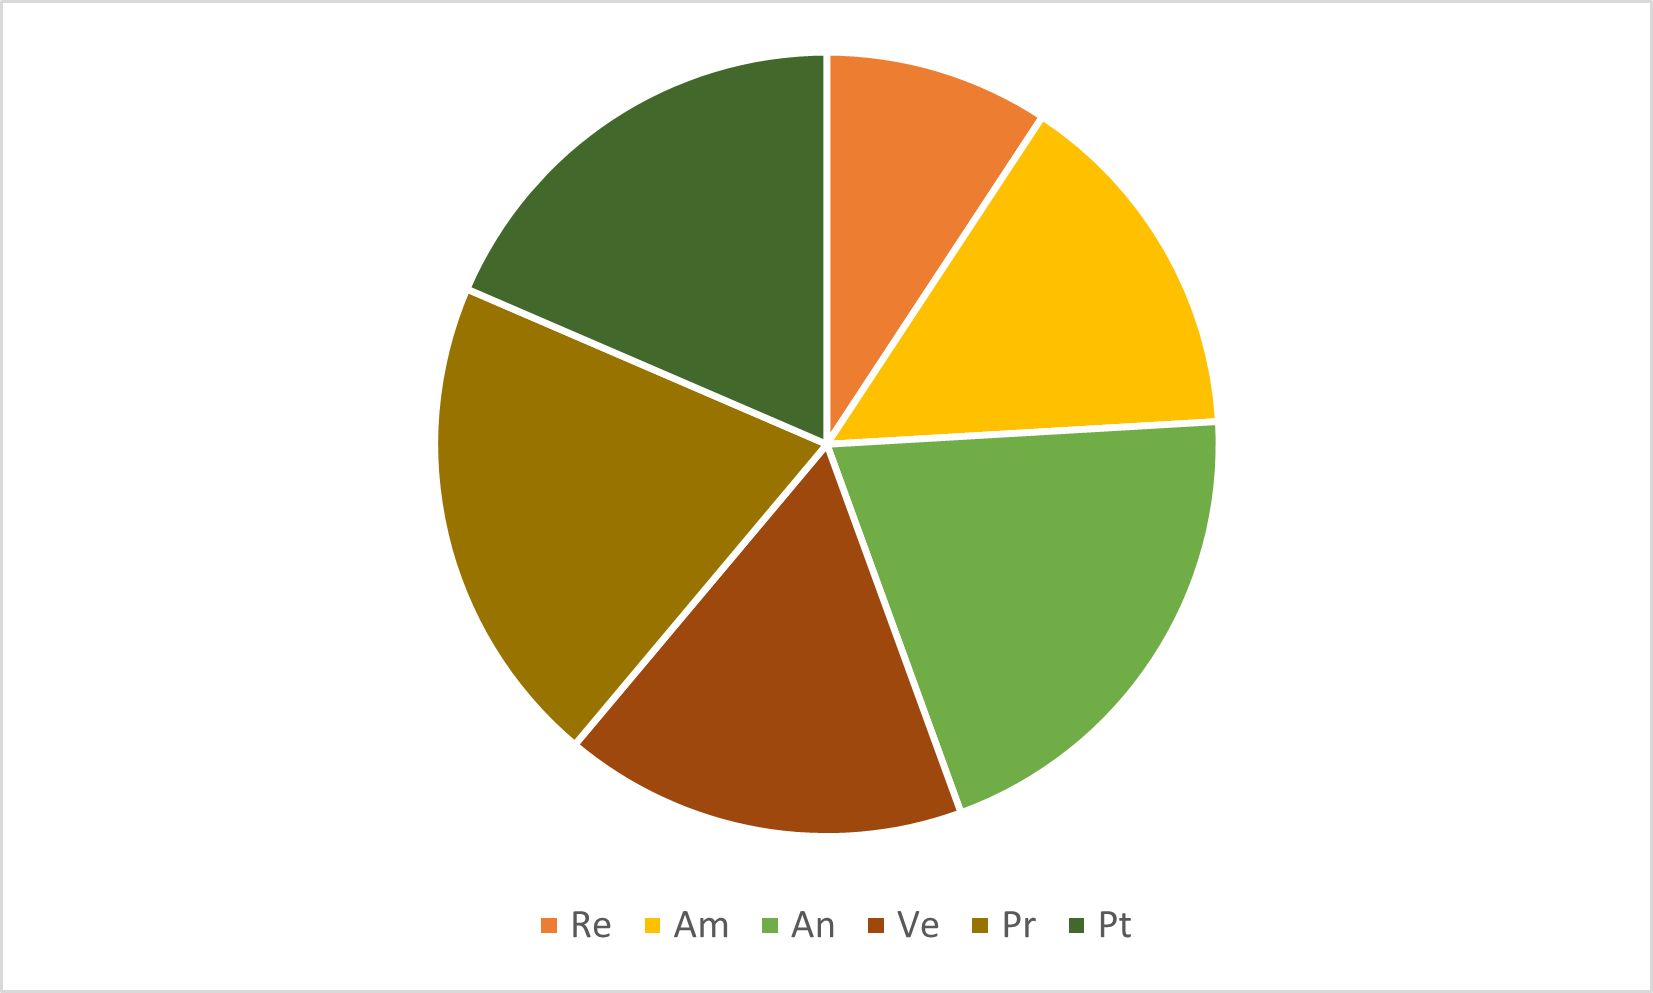
\includegraphics[scale=0.6]{img/grafi preventivo/torta/totale/totale.png}
    \caption{Grafico a torta della ripartizione delle ore per ruolo}
\end{figure}
\subsubsection{Preventivo dei costi}
La seguente tabella rappresenta le ore totali dedicate ad ogni ruolo e il corrispettivo costo in euro:

	\setlength\extrarowheight{5pt}
	\rowcolors{2}{gray!10}{gray!40}
	\begin{tabularx}{\textwidth}{|ccc|c|}
		\hline
		\rowcolor{white}
		\textbf{Ruolo} & \textbf{Costo orario (€)} & \textbf{Ore totali} & \textbf{Costo totale (€)} \\
		\hline
		Responsabile &30&50&1500 \\
		Amministratore &20&80&1600 \\
		Analista &25&110&2750 \\
		Verificatore &15&90&1350 \\
		Programmatore &15&110&1650 \\
		Progettista &25&100&2500 \\
		\hline
		Totale &-&-&11350 \\
		\hline
		\rowcolor{white}
		\caption{Prospetto del costo orario per ruolo totale}
	\end{tabularx}
    \vspace{10pt}
	
% ----------------------------------------------------------------------------------------------------------------
